\documentclass[hidelinks,a4paper,12pt]{article}

%***********************************************PACKAGES***************************************

\usepackage[left=2in, right=1in, top=1in, bottom=1in]{geometry}
\usepackage[table]{xcolor}
\usepackage{graphicx}
\usepackage{sectsty} %to customise headings
\usepackage{times} %this is for the selection of font
\usepackage{float}
\usepackage{fancyhdr}	
\usepackage[ampersand]{easylist}
\usepackage{amssymb}
\usepackage{enumitem}	
\usepackage{caption} \captionsetup[table]{singlelinecheck=false, margin=1em}
%\usepackage{tabu}
\usepackage{longtable}
\usepackage{booktabs}
\usepackage{eso-pic}
%\usepackage{transparent}
\usepackage{pdfpages}
\usepackage{tocloft}

\usepackage{ltablex}
\setlength{\LTpre}{0pt}
\setlength{\LTpost}{-15pt}

\usepackage{array}
\usepackage{tabularx}

\usepackage{chngcntr}
\counterwithin{table}{section}
\counterwithin{figure}{section}

\usepackage{rotating}
\usepackage{tikz}

\usepackage{upquote}
\usepackage[utf8]{inputenc}
\usepackage{listings}
\usepackage{listings-golang}

\usepackage{go/lang}  % include custom language for Go.
\usepackage{go/style} % include custom style for Go.
\usepackage{html/main} % include custom style for Html, CSS and Javascript

% glossary
\usepackage[acronym]{glossaries} 

\newglossaryentry{Electronic Commerce}{%
  name={Electronic Commerce (\textmd{also} e-commerce)},%
  description={commercial transactions conducted electronically on the Internet.}}
  
\newglossaryentry{computer network}{%
  name={Computer Network},%
  description={ a set of computers connected together for the purpose of sharing resources.}}  

\newglossaryentry{Internet}{%
  name={Internet},%
  description={ a global computer network providing a variety of information and communication facilities, consisting of interconnected networks using standardized communication protocols.}}    

\newglossaryentry{Social Networks}{%
  name={Social Networks},%
  description={a dedicated website or other application which enables users to communicate with each other by posting information, comments, messages, images, etc.}}      

\newglossaryentry{mobile commerce}{%
  name={Mobile Commerce},%
  description={M-commerce (mobile commerce) is the buying and selling of goods and services through wireless handheld devices such as cellular telephone and personal digital assistants (PDAs).}}      

\newglossaryentry{Supply Chain Management}{%
  name={Supply Chain Management},%
  description={Supply chain management (SCM) is the oversight of materials, information, and finances as they move in a process from supplier to manufacturer to wholesaler to retailer to consumer. }}        
  
\newglossaryentry{Internet Marketing}{%
  name={Internet Marketing},%
  description={Internet marketing, or online marketing, refers to advertising and marketing efforts that use the Web and email to drive direct sales via electronic commerce, in addition to sales leads from Web sites or emails.}}          
  
\newglossaryentry{Online Transaction Processing}{%
  name={Online Transaction Processing},%
  description={Online transaction processing, or OLTP, is a class of information systems that facilitate and manage transaction-oriented applications, typically for data entry and retrieval transaction processing.}}            
  
%\newglossaryentry{Electronic Data Interchange}{%
%name={Electronic Data Interchange},%
% description={Electronic Data Interchange (EDI) is the electronic interchange of business information using a standardized format; a process which allows one company to send information to another company electronically rather than with paper.}}     

\newglossaryentry{EDI}
{
    name={EDI},
    description={Electronic Data Interchange (EDI) is the electronic interchange of business information using a standardized format; a process which allows one company to send information to another company electronically rather than with paper.},
    first={Electronic Data Interchange (EDI)},
    long={Electronic Data Interchange}
}  
  
  
\newglossaryentry{Inventory Management}{%
  name={Inventory Management},%
  description={Inventory management is the supervision of non-capitalized assets (inventory) and stock items. A component of supply chain management, inventory management supervises the flow of goods from manufacturers to warehouses and from these facilities to point of sale.}}  
  
\newglossaryentry{World Wide Web}{%
  name={World Wide Web},%
  description={an information system on the Internet which allows documents to be connected to other documents by hypertext links, enabling the user to search for information by moving from one document to another.}}    

\newglossaryentry{email}{%
  name={Email},%
  text={email},
  description={messages distributed by electronic means from one computer user to one or more recipients via a network.}}     

\newglossaryentry{web browser}{%
  name={Web Browser},%
  description={a computer program with a graphical user interface for displaying HTML files, used to navigate the World Wide Web.}}       
  
\newglossaryentry{search engine}{%
  name={Search Engine},%
  description={a program that searches for and identifies items in a database that correspond to keywords or characters specified by the user, used especially for finding particular sites on the World Wide Web.}}         
  
\newglossaryentry{B2C}
{
    name={B2C},
    description={Business-to-consumer (B2C) is an Internet and electronic commerce (e-commerce) model that denotes a financial transaction or online sale between a business and consumer.},
    first={Business-to-consumer (B2C)},
    long={Business-to-consumer}
}  

\newglossaryentry{Paypal}{%
  name={Paypal},%
  description={Paypal is an electronic commerce (e-commerce) company that facilitates payments between parties through online funds transfers.}}      
  
\newglossaryentry{real-time transaction processing}{%
  name={Real-time transaction processing},%
  text={real-time transaction processing},
  description={In a real-time processing system, transactions are processed immediately as they occur without any delay to accumulate transactions.}}     
  
\newglossaryentry{SSL}
{
    name={SSL},
    description={Secure Sockets Layer (SSL) is the standard security technology for establishing an encrypted link between a web server and a browser.},
    first={SSL},
    long={Secure Sockets Layer}
}  

\newglossaryentry{Marketplace}{%
  name={Marketplace},%
  description={the arena of commercial dealings. An online marketplace (or online e-commerce marketplace) is a type of e-commerce site where product or service information is provided by multiple third parties, whereas transactions are processed by the marketplace operator.}}     

\newglossaryentry{web design}{%
  name={Web design},%
  text={web design},
  description={Web design is the process of creating websites. It encompasses several different aspects, including webpage layout, content production, and graphic design. While the terms web design and web development are often used interchangeably, web design is technically a subset of the broader category of web development.}}     
  
\newglossaryentry{web security}{%
  name={Web security},%
  text={web security},
  description={Web application security is a branch of Information Security that deals specifically with security of websites, web applications and web services. At a high level, Web application security draws on the principles of application security but applies them specifically to Internet and Web systems.}}       
  
\newglossaryentry{RDBMS}
{
    name={RDBMS},
    description={Relational Database management System (RDBMS) is a database management system based on relational model defined by E.F.Codd. Data is stored in the form of rows and columns. The relations among tables are also stored in the form of the table.},
    first={RDBMS},
    long={Relational Database management System}
}  
  
  
\newglossaryentry{OOP}
{
    name={OOP},
    description={Object-oriented programming (OOP) refers to a type of computer programming (software design) in which programmers define not only the data type of a data structure, but also the types of operations (functions) that can be applied to the data structure.},
    first={OOP},
    long={Object-oriented programming}
}

\newglossaryentry{Network security}{%
  name={Network security},%
  text={Network security},
  description={Network security is protection of the access to files and directories in a computer network against hacking, misuse and unauthorized changes to the system.}}      
  
\newglossaryentry{TLS}
{
    name={TLS},
    description={Transport layer security (TLS) is a protocol that provides communication security between client/server applications that communicate with each other over the Internet.},
    first={Transport Layer Security (TLS)},
    long={TLS}
}  

%*****************************************Section 2**************************************************  
  
\newglossaryentry{broadband}{%
  name={Broadband},%
  text={broadband},
  description={a high-capacity transmission technique using a wide range of frequencies, which enables a large number of messages to be communicated simultaneously.}}        

\newglossaryentry{e-commerce}
    {name=e-commerce,description={\emph{See} \gls{Electronic Commerce}}}  
  
\newglossaryentry{4G}
{
    name={4G},
    description={4\textsuperscript{th} Generation (4G) is a mobile communications standard intended to replace 3G, allowing wireless Internet access at a much higher speed.},
    first={4G},
    long={4G}
}   

\newglossaryentry{social media}{%
  name={Social Media},%
  text={social media},
  description={websites and applications that enable users to create and share content or to participate in social networking.}}            

\newglossaryentry{go-live}{%
  name={Go-live},%
  text={go-live},  
  description={(of a computer system) become operational.}}            
  
\newglossaryentry{i686}{%
  name={i686},
  description={i686 is widely used to describe 32-bit P6 processor architecture which is compatible with Pentium Pro/II and has it's instruction set.}}    
  
\newglossaryentry{Linux}{%
  name={Linux},
  description={an open-source operating system modelled on UNIX.}}    
  
\newglossaryentry{Operating System}{%
  name={Operating System},
  description={the low-level software that supports a computer`s basic functions, such as scheduling tasks and controlling peripherals.}}      
  
\newglossaryentry{API}
{
    name={API},
    description={In computer programming, an application programming interface (API) is a set of functions and procedures that allow the creation of applications which access the features or data of an operating system, application, or other service.},
    first={API},
    long={Application Programming Interface}
}   

\newglossaryentry{Payment Gateway}{%
  name={Payment Gateway},
  description={A payment gateway is a merchant service provided by an e-commerce application service provider that authorizes credit card or direct payments processing for e-businesses, online retailers, bricks and clicks, or traditional brick and mortar.}}      
  
\newglossaryentry{Web server}{%
  name={Web server},
  description={A Web server is a program that uses HTTP (Hypertext Transfer Protocol) to serve the files that form Web pages to users, in response to their requests, which are forwarded by their computers` HTTP clients. }}        
  
\newglossaryentry{PSP}
{
    name={PSP},
    description={The Personal Software Process (PSP) is a structured software development process that is intended (planned) to help software engineers better understand and improve their performance by tracking their predicted and actual development of code.},
    first={Personal Software Process (PSP)},
    long={Personal Software Process}
}   

\newglossaryentry{Hosting}{%
  name={Hosting},
  description={store (a website or other data) on a server or other computer so that it can be accessed over the Internet.}}       

\newglossaryentry{Software Requirement Specifications}{%
  name={Software Requirement Specifications},
  description={store (A software requirements specification (SRS) is a description of a software system to be developed. It lays out functional and non-functional requirements, and may include a set of use cases that describe user interactions that the software must provide.}}         

\newglossaryentry{HTTPS}
{
    name={HTTPS},
    description={HTTPS (HTTP over SSL or HTTP Secure) is the use of Secure Socket Layer (SSL) or Transport Layer Security (TLS) as a sublayer under regular HTTP application layering. HTTPS encrypts and decrypts user page requests as well as the pages that are returned by the Web server.},
    first={HTTPS},
    long={HTTP over SSL or HTTP Secure}
}   

\newglossaryentry{authenticate}{%
  name={Authentication},%
  text={authenticate},
  description={the process or action of verifying the identity of a user or process.}}         


\newglossaryentry{session}{%
  name={Session},
  text={session},
  description={the period of activity between a user logging in and logging out of a (multi-user) system.}}         

\newglossaryentry{UUID}
{
    name={UUID},
    description={A UUID (Universal Unique Identifier) is a 128-bit number used to uniquely identify some object or entity on the Internet. },
    first={UUID},
    long={Universal Unique Identifier}
}     

\newglossaryentry{CMM}
{
    name={CMM},
    description={The Capability Maturity Model (CMM) is a methodology used to develop and refine an organization's software development process. The model describes a five-level evolutionary path of increasingly organized and systematically more mature processes.},
    first={Capability Maturity Model (CMM)},
    long={Capability Maturity Model}
}

\newglossaryentry{TSP}
{
    name={TSP},
    description={n combination with the personal software process (PSP), the team software process (TSP) provides a defined operational process framework that is designed to help teams of managers and engineers organize projects and produce software products that range in size from small projects of several thousand lines of code (KLOC) to very large projects greater than half a million lines of code},
    first={ team software process (TSP)},
    long={team software process}
}

\newglossaryentry{garbage collection}{%
  name={Garbage collection},
  text={garbage collection},
  description={the automatic process of making space in a computer's memory by removing data that is no longer required or in use.}}         

\newglossaryentry{statically typed}{%
  name={Statically typed},
  text={statically typed},
  description={Enforcement of type rules at compile time rather than at run time. Static typing catches more errors at compile time than dynamic typing.}}        

\newglossaryentry{open source}{%
  name={Open source},
  text={open source},
  description={denoting software for which the original source code is made freely available and may be redistributed and modified.}}          

\newglossaryentry{object file}{%
  name={Object file},
  text={object file},
  description={An object file is a file containing object code, meaning relocatable format machine code that is usually not directly executable.}}  

\newglossaryentry{compiler}{%
  name={Compiler},
  text={compiler},
  description={a program that converts instructions into a machine-code or lower-level form so that they can be read and executed by a computer}}    
  
\newglossaryentry{linker}{%
  name={Linker},
  text={linker},
  description={a program used with a compiler or assembler to provide links to the libraries needed for an executable program.}}    
  
\newglossaryentry{namespaces}{%
  name={Namespaces},
  text={namespaces},
  description={A namespace in computer science (sometimes also called a name scope), is an abstract container or environment created to hold a logical grouping of unique identifiers or symbols.}}           

\newglossaryentry{URL}
{
    name={URL},
    description={A URL (Uniform Resource Locator), as the name suggests, provides a way to locate a resource on the web, the hypertext system that operates over the internet.},
    first={URL},
    long={Uniform Resource Locator }
}  

\newglossaryentry{type information}{%
  name={Type information},
  text={type information},
  description={In computer programming, run-time type information refers to a mechanism that exposes information about an object`s data type at runtime. Run-time type information can apply to simple data types, such as integers and characters, or to generic types.}}          


\newglossaryentry{symbol table}{%
  name={Symbol table},
  text={symbol table},
  description={In computer science, a symbol table is a data structure used by a language translator such as a compiler or interpreter, where each identifier (a.k.a. symbol) in a program`s source code is associated with information relating to its declaration or appearance in the source.}}         

\newglossaryentry{first-class functions}{%
  name={First-class functions},
  text={first-class functions},
  description={Specifically, this means the language supports passing functions as arguments to other functions, returning them as the values from other functions, and assigning them to variables or storing them in data structures. It means that functions are objects, with a type and a behaviour. They can be dynamically built, passed around as any other object, and the fact that they can be called is part of their interface. }}            

\newglossaryentry{closures}{%
  name={Closures},
  text={closures},
  description={In computer science, a closure is a function that has an environment of its own. Inside this environment, there is at least one bound variable.}}    

\newglossaryentry{type-safe}{%
  name={Type-safe},
  text={type-safe},
  description={Type-Safe is code that accesses only the memory locations it is authorized to access, and only in well-defined, allowable ways.}}              
  
\newglossaryentry{variadic functions}{%
  name={Variadic functions},
  text={variadic functions},
  description={In computer science, an operator or function is variadic if it can take a varying number of arguments; that is, if its arity is not fixed.}}  
  
\newglossaryentry{identifier}{%
  name={Identifier},
  text={identifier},
  description={An identifier is the user-defined name of a program element. It can be a namespace, class, method, variable or interface. Identifiers are symbols used to uniquely identify a program element in the code. They are also used to refer to types, constants, macros and parameters.}}   

\newglossaryentry{reflection}{%
  name={Reflection},
  text={reflection},
  description={In computer science, reflection is the ability of a computer program to examine, introspect, and modify its own structure and behavior at runtime.}}     
  
\newglossaryentry{Concurrency}{%
  name={Concurrency},
  description={In computer science, concurrency is the execution of several instruction sequences at the same time. In an operating system, this happens when there are several process threads running in parallel. These threads may communicate with each other through either shared memory or message passing.}}       

\newglossaryentry{Composition}{%
  name={Composition},
  description={In computer science, function composition is an act or mechanism to combine simple functions to build more complicated ones. Object composition is a way to combine simple objects or data types into more complex ones.}}   

\newglossaryentry{inheritance}{%
  name={Inheritance},
  text={inheritance},
  description={In object-oriented programming, inheritance enables new objects to take on the properties of existing objects.}}                         

\newglossaryentry{error handling}{%
  name={Error handling},
  text={error handling},
  description={Error handling refers to the anticipation, detection, and resolution of programming, application, and communications errors.}}                   

%******************************************************Section******************************************

\newglossaryentry{cryptographic protocols}{%
  name={Cryptographic protocols},
  text={cryptographic protocols},
  description={A security protocol (cryptographic protocol or encryption protocol) is an abstract or concrete protocol that performs a security-related function and applies cryptographic methods, often as sequences of cryptographic primitives. }}                         

\newglossaryentry{OpenSSL}{%
  name={OpenSSL},
  text={OpenSSL},
  description={OpenSSL is a software library to be used in applications that need to secure communications over computer networks against eavesdropping or need to ascertain the identity of the party at the other end. }}      
  
\newglossaryentry{encryption}{%
  name={Encryption},
  text={encryption},
  description={the process of converting information or data into a code, especially to prevent unauthorized access.}}        
  
\newglossaryentry{algorithm}{%
  name={Algorithm},
  text={algorithm},
  description={a process or set of rules to be followed in calculations or other problem-solving operations, especially by a computer.}}          
  
\newglossaryentry{public-key cryptography}{%
  name={Public-key cryptography (\textmd{also} asymmetric cipher)},
  text={public-key cryptography},
  description={Public key cryptography, or asymmetric cryptography, is any cryptographic system that uses pairs of keys: public keys which may be disseminated widely, and private keys which are known only to the owner.}}          

\newglossaryentry{asymmetric cipher}
    {name=asymmetric cipher,description={\emph{See} \gls{public-key cryptography}}}      

\newglossaryentry{message authentication code}{%
  name={Message Authentication Code},
  text={message authentication code},
  description={In cryptography, a message authentication code (MAC) is a short piece of information used to authenticate a message—in other words, to confirm that the message came from the stated sender (its authenticity) and has not been changed in transit (its integrity).}}    

\newglossaryentry{forward secrecy}{%
  name={Forward Secrecy},
  text={forward secrecy},
  description={In cryptography, forward secrecy (FS; also known as perfect forward secrecy) is a property of secure communication protocols in which compromise of long-term keys does not compromise past session keys. Forward secrecy protects past sessions against future compromises of secret keys or passwords.}}               

\newglossaryentry{TLS record protocol}{%
  name={TLS record protocol},
  text={TLS record protocol},
  description={The Transport Layer Security (TLS) Record protocol secures application data using the keys created during the Handshake.}}
  
\newglossaryentry{TLS handshake protocol}{%
  name={TLS handshake protocol},
  text={TLS handshake protocol},
  description={The Transport Layer Security (TLS) Handshake Protocol is responsible for the authentication and key exchange necessary to establish or resume secure sessions.}}                 
  
\newglossaryentry{stateful connection}{%
  name={Stateful Connection},
  text={stateful connection},
  description={A stateful connection is one in which some information about a connection between two systems is retained for future use}}      
  
\newglossaryentry{symmetric cipher}{%
  name={Symmetric cipher},
  text={symmetric cipher},
  description={Symmetric ciphers are the oldest and most used cryptographic ciphers. In a symmetric cipher, the key that deciphers the ciphertext is the same as (or can be easily derived from) the key enciphers the clear text. This key is often referred to as the secret key.}}    
  
\newglossaryentry{session key}{%
  name={Session key},
  text={session key},
  description={A session key is an encryption and decryption key that is randomly generated to ensure the security of a communications session between a user and another computer or between two computers. Session keys are sometimes called symmetric keys, because the same key is used for both encryption and decryption.}}    
  
\newglossaryentry{handshake}{%
  name={Handshake},
  text={handshake},
  description={The handshaking process usually takes place in order to establish rules for communication when a computer sets about communicating with a foreign device. When a computer communicates with another device like a modem, printer, or network server, it needs to handshake with it to establish a connection.}}          

\newglossaryentry{client}{%
  name={Client},
  text={client},
  description={(in a network) a desktop computer or workstation that is capable of obtaining information and applications from a server.}}  

\newglossaryentry{hash functions}{%
  name={Hash functions},
  text={hash functions},
  description={A hash function is any function that can be used to map data of arbitrary size to data of fixed size. The values returned by a hash function are called hash values, hash codes, digests, or simply hashes.}}      

\newglossaryentry{digital certificate}{%
  name={Digital Certificate},
  text={digital certificate},
  description={In cryptography, a public key certificate (also known as a digital certificate or identity certificate) is an electronic document used to prove the ownership of a public key.}}        


\newglossaryentry{CA}
{
    name={CA},
    description={Certificate Authorities (CA) issue Digital Certificates. A certificate authority (CA) is a trusted entity that issues electronic documents that verify a digital entity`s identity on the Internet. The electronic documents, which are called digital certificates, are an essential part of secure communication and play an important part in the public key infrastructure (PKI).},
    first={Certificate Authority (CA) },
    long={Certificate Authority}
}    

\newglossaryentry{decrypt}{%
  name={Decryption},
  text={decrypt},
  description={Decryption is the process of taking encoded or encrypted text or other data and converting it back into text that you or the computer can read and understand. This term could be used to describe a method of un-encrypting the data manually or with un-encrypting the data using the proper codes or keys.}}  
  
\newglossaryentry{private key}{%
  name={Private Key},
  text={private key},
  description={A private key is a tiny bit of code that is paired with a public key to set off algorithms for text encryption and decryption. It is created as part of public key cryptography during asymmetric-key encryption and used to decrypt and transform a message to a readable format.}}    
  
  
\newglossaryentry{Diffie-Hellman key exchange}{%
  name={Diffie-Hellman key exchange},
  text={Diffie-Hellman key exchange},
  description={Diffie–Hellman key exchange (D–H) is a specific method of securely exchanging cryptographic keys over a public channel and was one of the first public-key protocols as originally conceptualized by Ralph Merkle and named after Whitfield Diffie and Martin Hellman.}}      
  

\newglossaryentry{X.509 certificates}{%
  name={X.509 certificates},
  text={X.509 certificates},
  description={In cryptography, X.509 is an important standard for a public key infrastructure (PKI) to manage digital certificates and public-key encryption and a key part of the Transport Layer Security protocol used to secure web and email communication.}}   

%***********************************************Section***********************************************  
  
\newglossaryentry{PROBE}{%
  name={PROBE},
  text={PROBE},
  description={Proxy-Based Estimating (PROBE) is an estimating process used in the Personal Software Process (PSP) to estimate size and effort.}}       
  
\newglossaryentry{linear regression}{%
  name={Linear regression},
  text={linear regression},
  description={In statistics, linear regression is an approach for modeling the relationship between a scalar dependent variable y and one or more explanatory variables (or independent variables) denoted X.}}   
  
\newglossaryentry{LOC}
{
    name={LOC},
    description={Source lines of code (SLOC), also known as lines of code (LOC), is a software metric used to measure the size of a computer program by counting the number of lines in the text of the program's source code.},
    first={Lines of Code (LOC) },
    long={Lines of Code}
}   

\newglossaryentry{correlation}{%
  name={Correlation},
  text={correlation},
  description={A correlation is a single number that describes the degree of relationship between two variables}}    
  
%********************************************************Section***********************************

\newglossaryentry{Gantt chart}{%
  name={Gantt Chart},
  text={Gantt chart},
  description={a chart in which a series of horizontal lines shows the amount of work done or production completed in certain periods of time in relation to the amount planned for those periods.}}  

\newglossaryentry{PERT}   
{
    name={PERT},
    description={The program (or project) evaluation and review technique, commonly abbreviated PERT, is a statistical tool, used in project management, which was designed to analyze and represent the tasks involved in completing a given project.},
    first={The program (or project) evaluation and review technique (PERT) },
    long={The program (or project) evaluation and review technique}
}   

%********************************************************Section************************************** 

\newglossaryentry{Single-Sign On}{%
  name={Single-Sign On},
  text={Single-Sign On (SSO)},
  description={Single sign-on (SSO) is a session and user authentication service that permits a user to use one set of login credentials (e.g., name and password) to access multiple applications.}}  

\newglossaryentry{persistent}{%
  name={Persistent},
  description={Persistent shopping carts save a customer`s cart contents across sessions through ``persistent cookies.`` A cookie is a small text file stored on a user`s computer. In computer science, persistence refers to the characteristic of state that outlives the process that created it. This is achieved in practice by storing the state as data in computer data storage. Programs have to transfer data to and from storage devices and have to provide mappings from the native programming-language data structures to the storage device data structures}}     

\newglossaryentry{Digital Wallets}{%
  name={Digital Wallet},
  text={Digital Wallets},
  description={A digital wallet refers to an electronic device that allows an individual to make electronic transactions. This can include purchasing items on-line with a computer or using a smartphone to purchase something at a store. An individual's bank account can also be linked to the digital wallet.}}    
  
  
\newglossaryentry{Responsive Web Design}{%
  name={Responsive Web Design},
  text={Responsive Web Design (RWD)},
  description={Responsive web design (RWD) is an approach to web design aimed at allowing desktop webpages to be viewed in response to the size of the device one is viewing with.}}     
  
\newglossaryentry{GPS}  
{
    name={GPS},
    description={The Global Positioning System (GPS) is a space-based radionavigation system owned by the United States Government (USG) and operated by the United States Air Force (USAF)},
    first={GPS},
    long={The Global Positioning System (GPS)}
}     
  
  
\makeglossaries

%**********************************************COMMANDS****************************************

\newcounter{functionalrequirement}
\renewcommand{\thefunctionalrequirement}{FR\arabic{functionalrequirement}}
\newcommand{\newFR}{%
  \refstepcounter{functionalrequirement}%
  \thefunctionalrequirement}

%**********************************************GRAPHS and PLOTS*********************************

\usepackage{pgfplots, pgfplotstable}
%\usepackage{makecell}
\usetikzlibrary{backgrounds}
% background color definition from pgfmanual-en-macros.tex
\definecolor{graphicbackground}{cmyk}{0,0,0,.03}
% key to change color
\pgfkeys{/tikz/.cd,
	background color/.initial=graphicbackground,
	background color/.get=\backcol,
	background color/.store in=\backcol,
}
\tikzset{background rectangle/.style={
		fill=\backcol,
	},
	use background/.style={    
		show background rectangle
	}
}


%****************************************************STYLING*****************************************

%\usepackage{lipsum}% Used for dummy text.

\definecolor{titlepagecolor}{cmyk}{1,.60,0,.40}
\definecolor{namecolor}{cmyk}{0.4,.2,0.,.10} 
\definecolor{levelfirst}{cmyk}{0,0,0,0.70}
\definecolor{levelSecond}{cmyk}{1,.50,0,.10}
\definecolor{levelthird}{cmyk}{1,.50,0,.10}
\definecolor{levelfourth}{cmyk}{1,.50,0,.10}
\definecolor{levelfifth}{cmyk}{1,.50,0,.10}

\definecolor{tablecell1}{cmyk}{0.07,0.03,0.03,0.07}
\definecolor{tablecell2}{cmyk}{0.04,0.02,0.02,0.04}



\sectionfont{\fontsize{16}{22}\selectfont}
\subsectionfont{\fontsize{14}{18}\selectfont}
\subsubsectionfont{\fontsize{12}{16}\selectfont}

\ListProperties(Hide=100, Hang=true, Progressive=6ex, Space=0.8em,Space*=0.8em, Style*=$\bullet$, Style2*=$\bullet$ ,Style3*=$\bullet$ ,Style4*=\tiny$\blacksquare$ )

% format Go Code
%\lstset{ 

%\lstdefinestyle{Go}{ %
	%frame=single,
	%aboveskip=3mm,
	%belowskip=3mm,			
	%columns=flexible,
 	%basicstyle={\small\ttfamily}, %basicstyle={\small\ttfamily} basicstyle=\footnotesize
	%keywordstyle=\color{red},
	%numbers=left,              %numbers=none
	%numbersep=5pt,
	%numberstyle=\tiny\color{gray},
	%showstringspaces=false, 
	%stringstyle=\color{blue},
	%commentstyle=\color{brown},
  	%breaklines=true,
  	%breakatwhitespace=true,	
	%tabsize=4,
	%language=Golang 
    %}

%***************************************************DOCUMENTATION************************************

\begin{document}

\begin{titlepage}
\thispagestyle{empty}
\pagenumbering{roman}

\hspace{-0.5in}

\includegraphics[ width= 0.78\paperwidth , keepaspectratio ]{./Images/TitlePage.png}
	
\end{titlepage}

\newpage
\hspace{-0.75in}
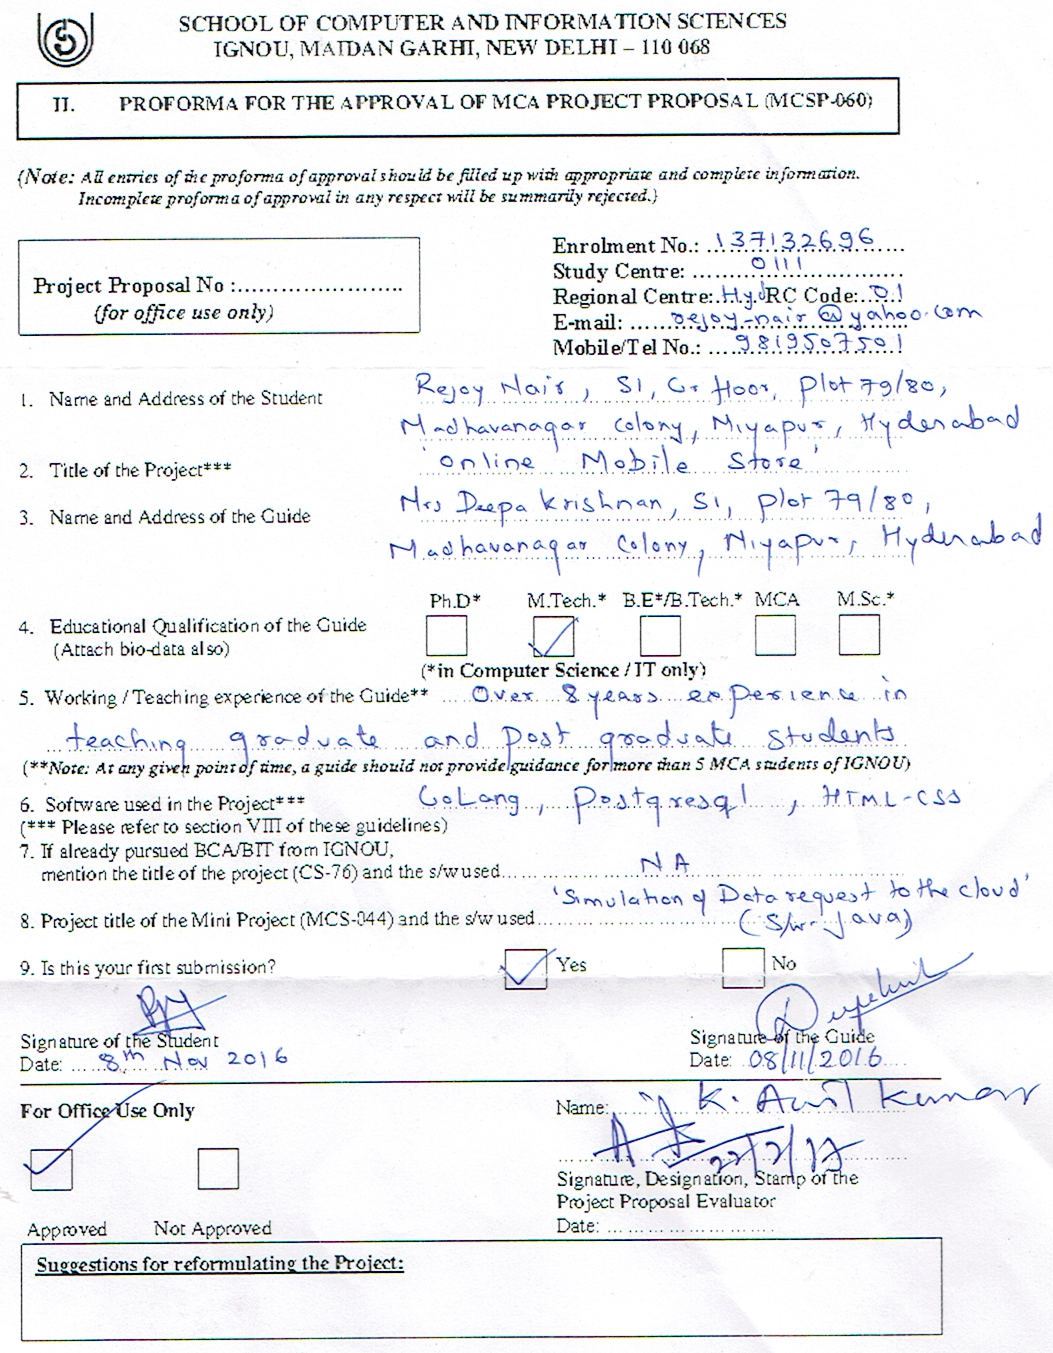
\includegraphics[ width= 0.82\paperwidth , keepaspectratio ]{./Images/Approval.png}
\newpage
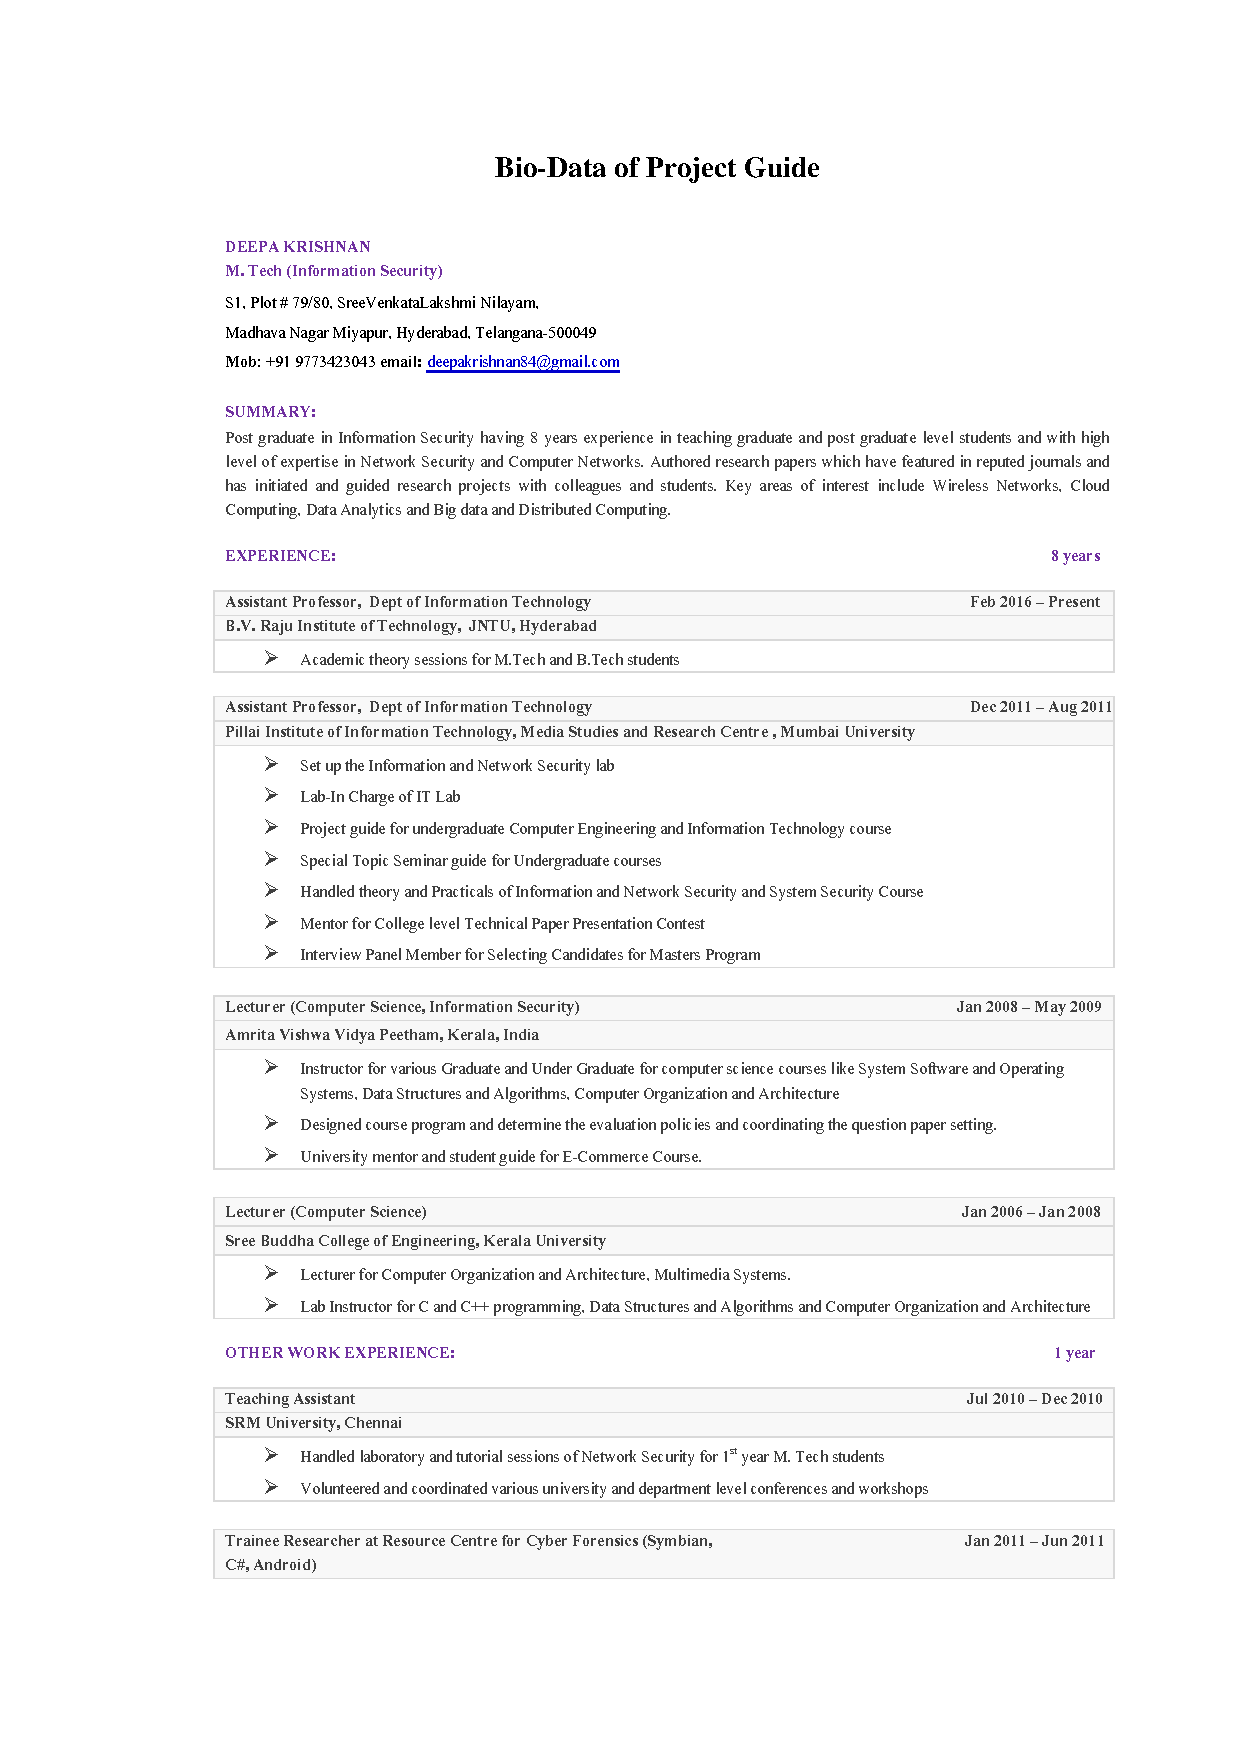
\includepdf[pagecommand={\thispagestyle{plain}}, pages={1,2}]{./Images/guidecv.pdf}
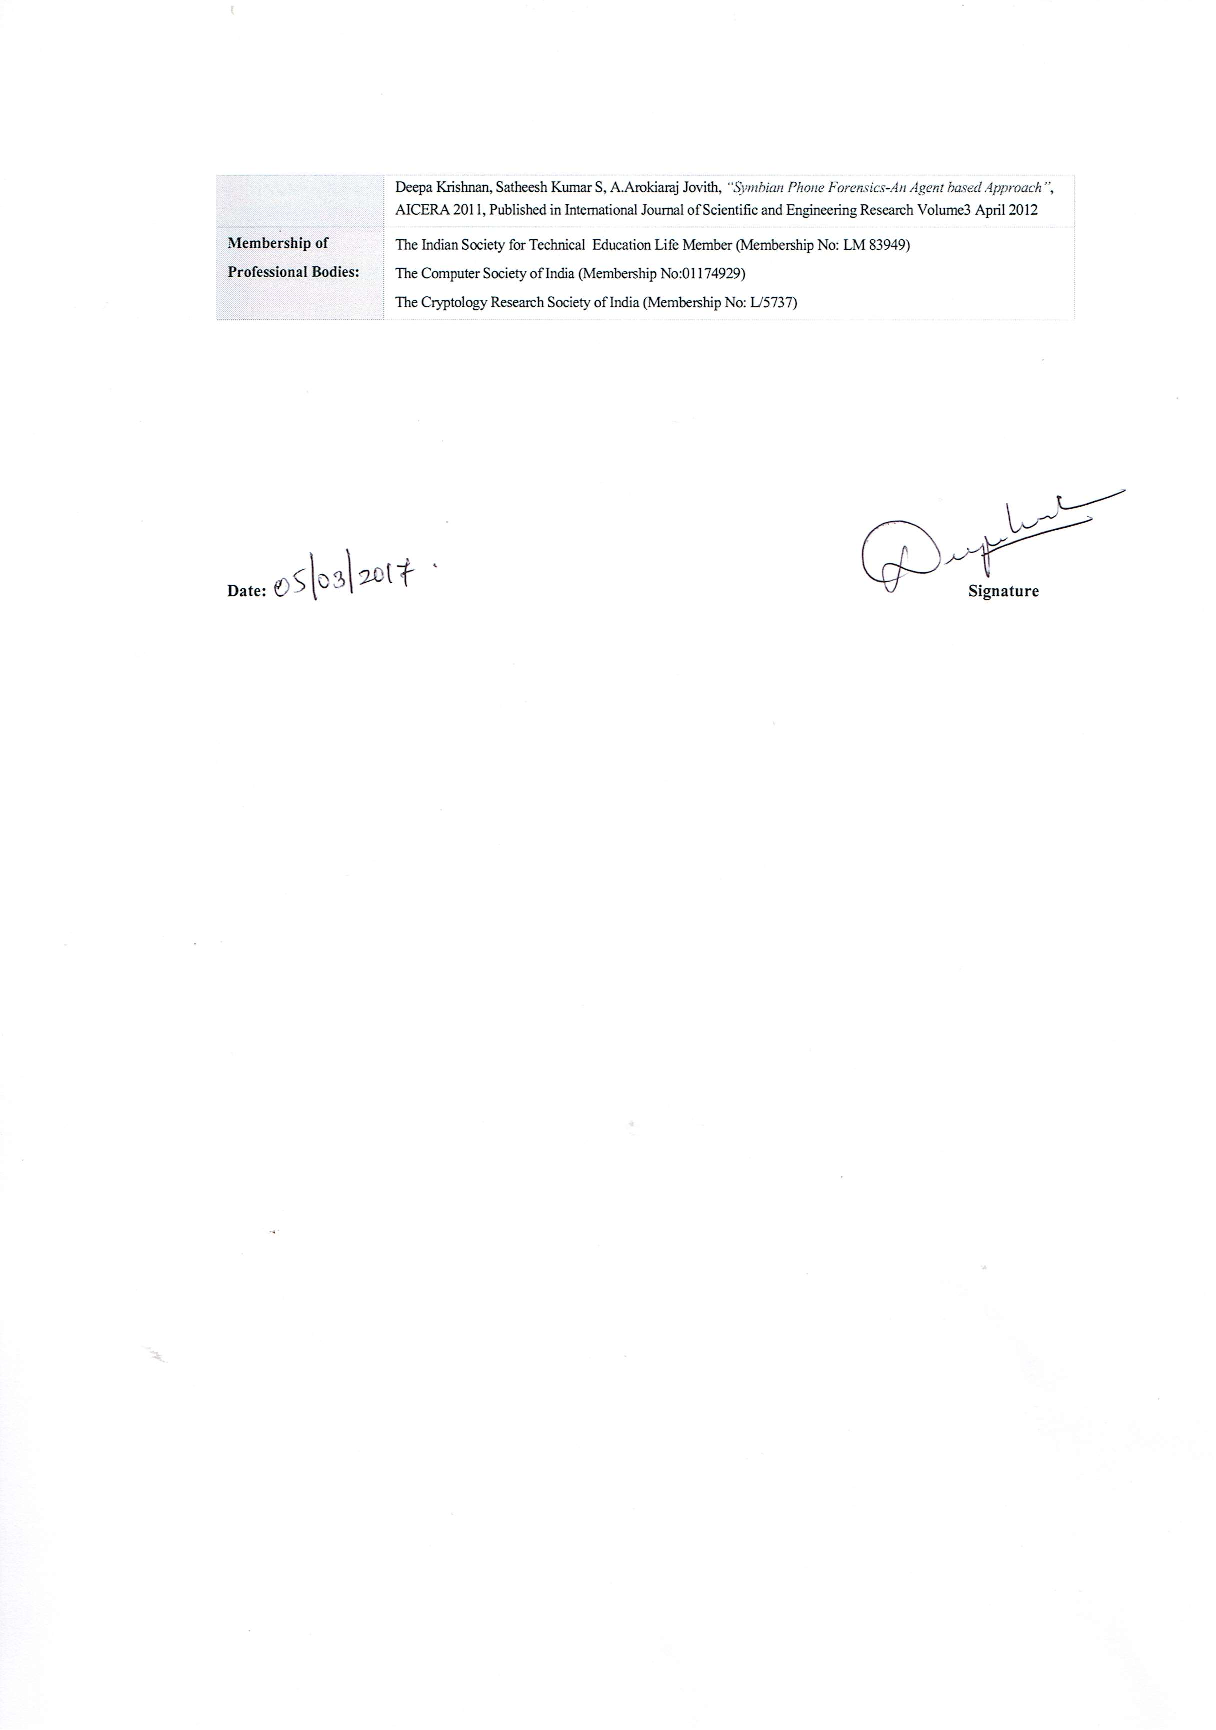
\includepdf[pagecommand={\thispagestyle{plain}}, pages={1}]{./Images/guidecvsigned.pdf}
\newpage
%\setcounter{page}{5}
\begin{center}
\hspace{-0.75in}
%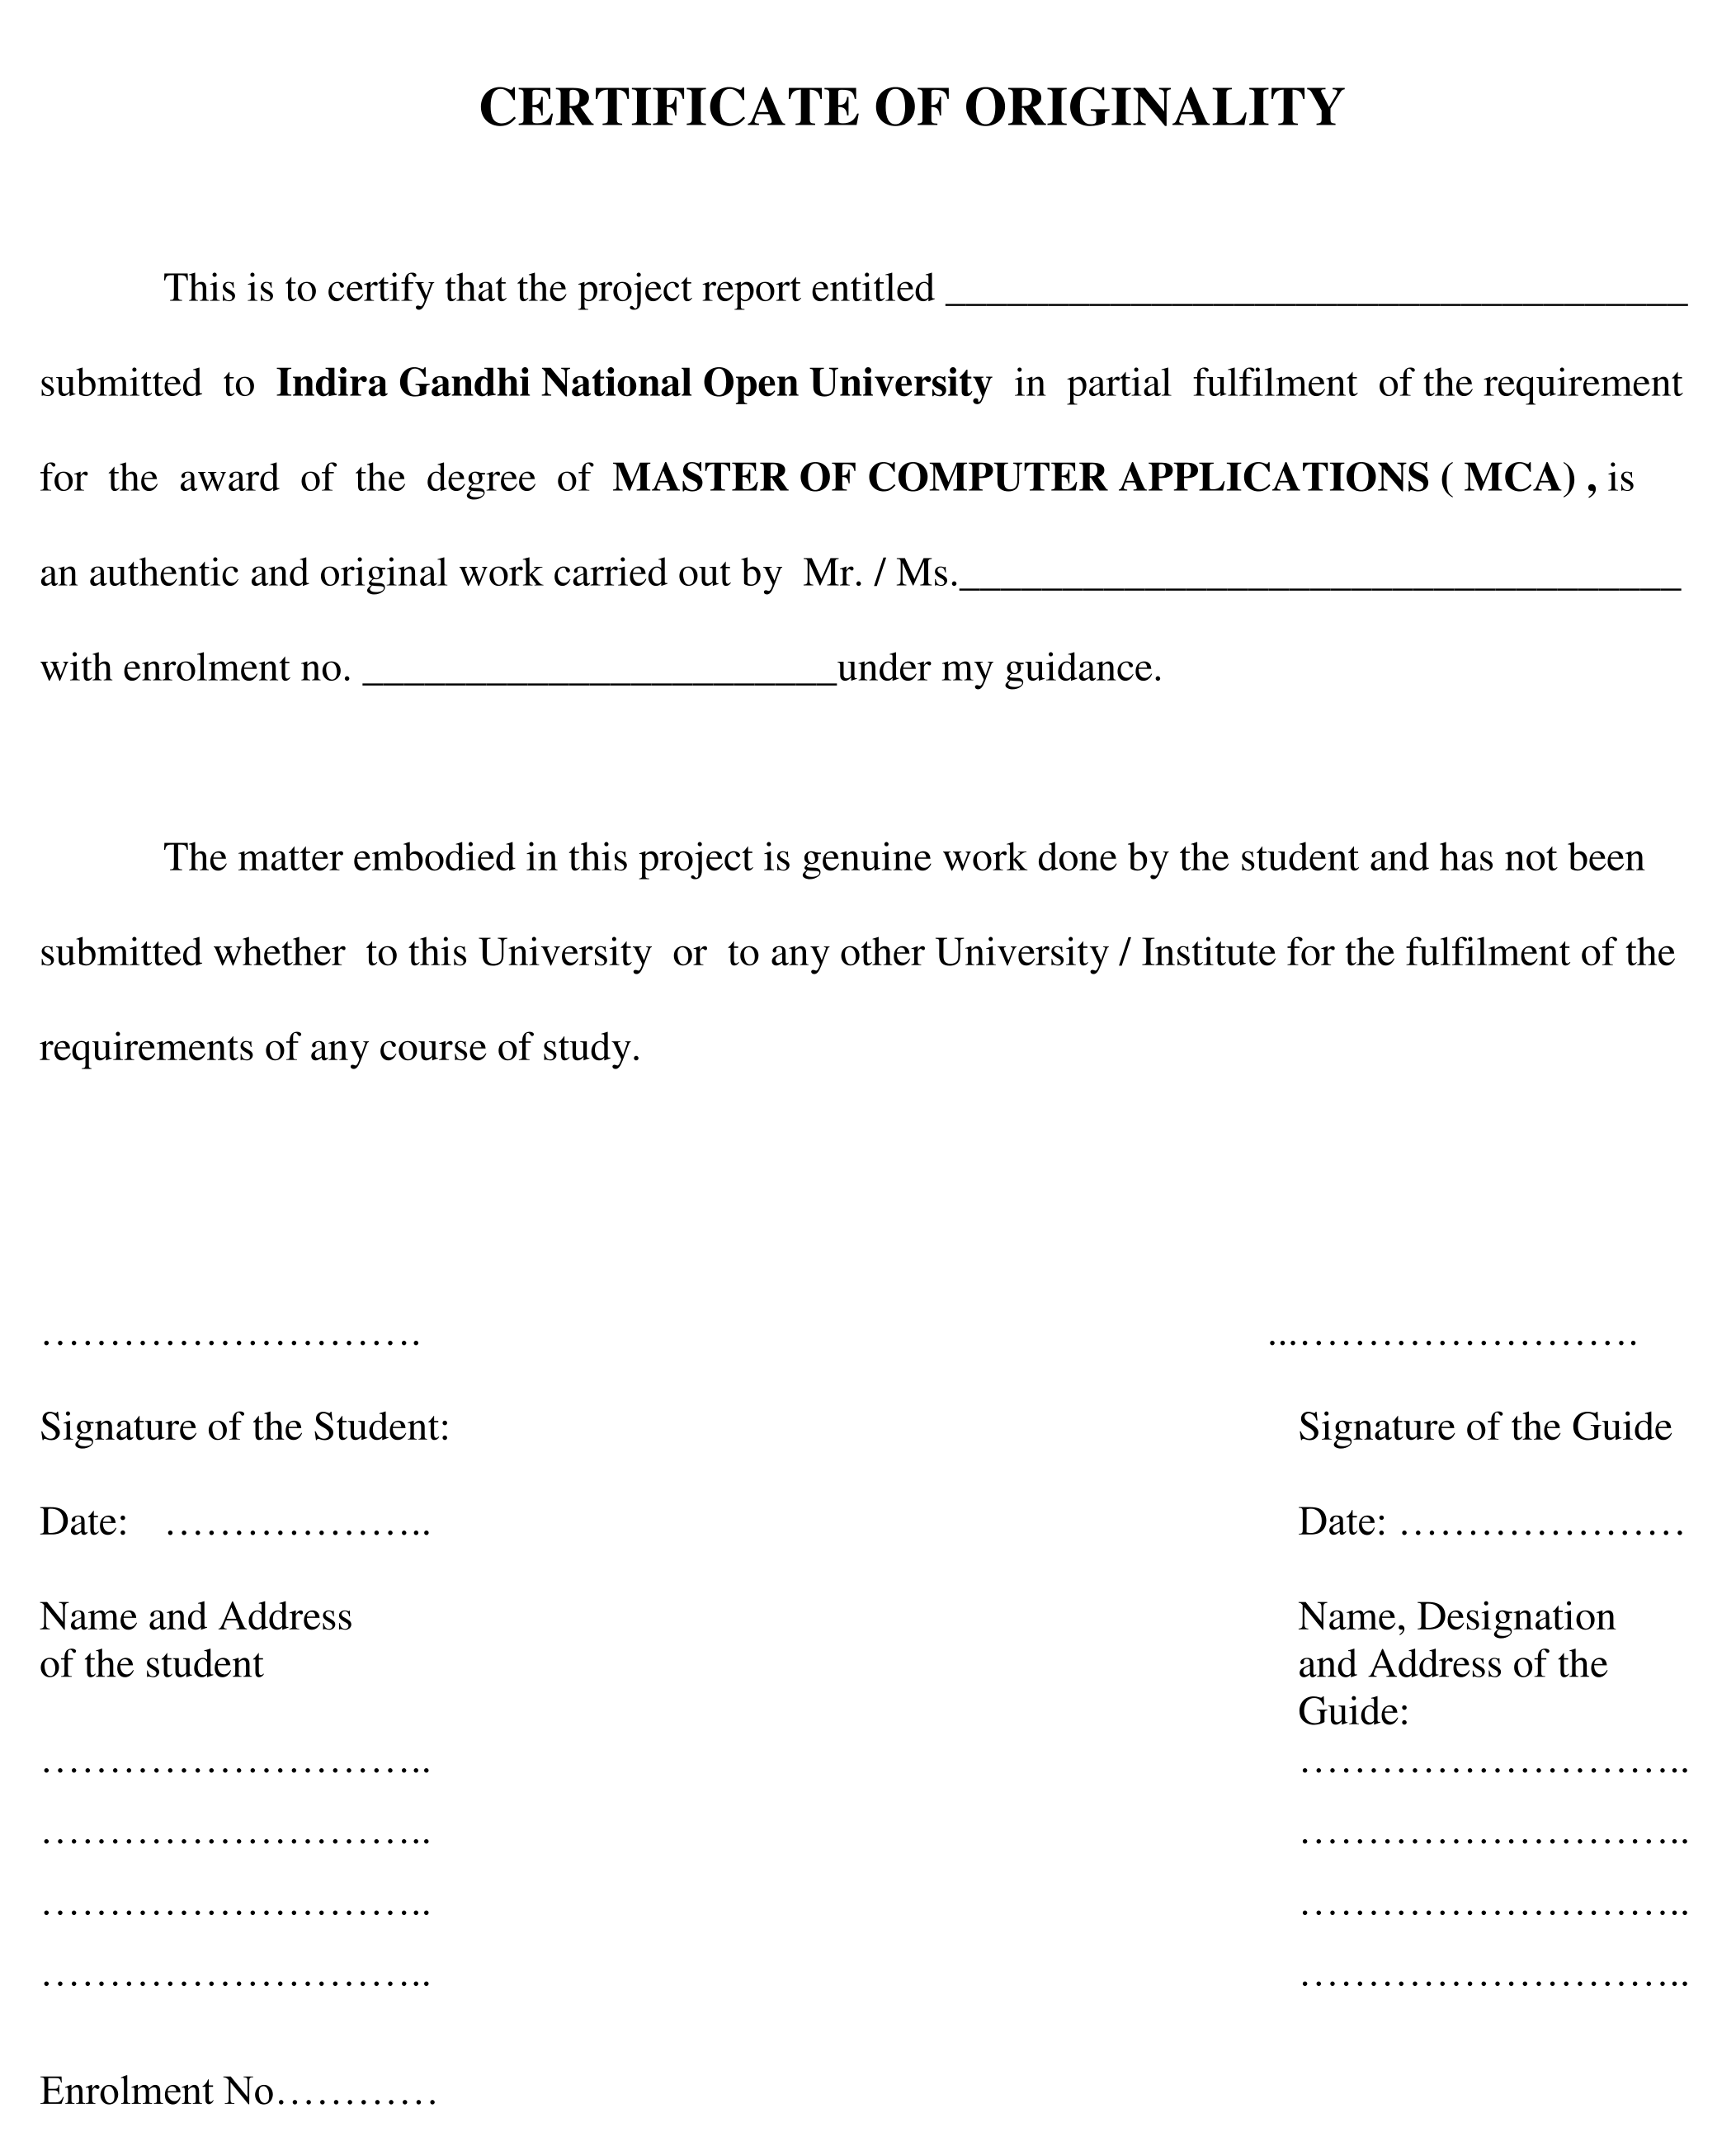
\includegraphics[ width= 0.76\paperwidth , keepaspectratio ]{./Images/CoO.png}
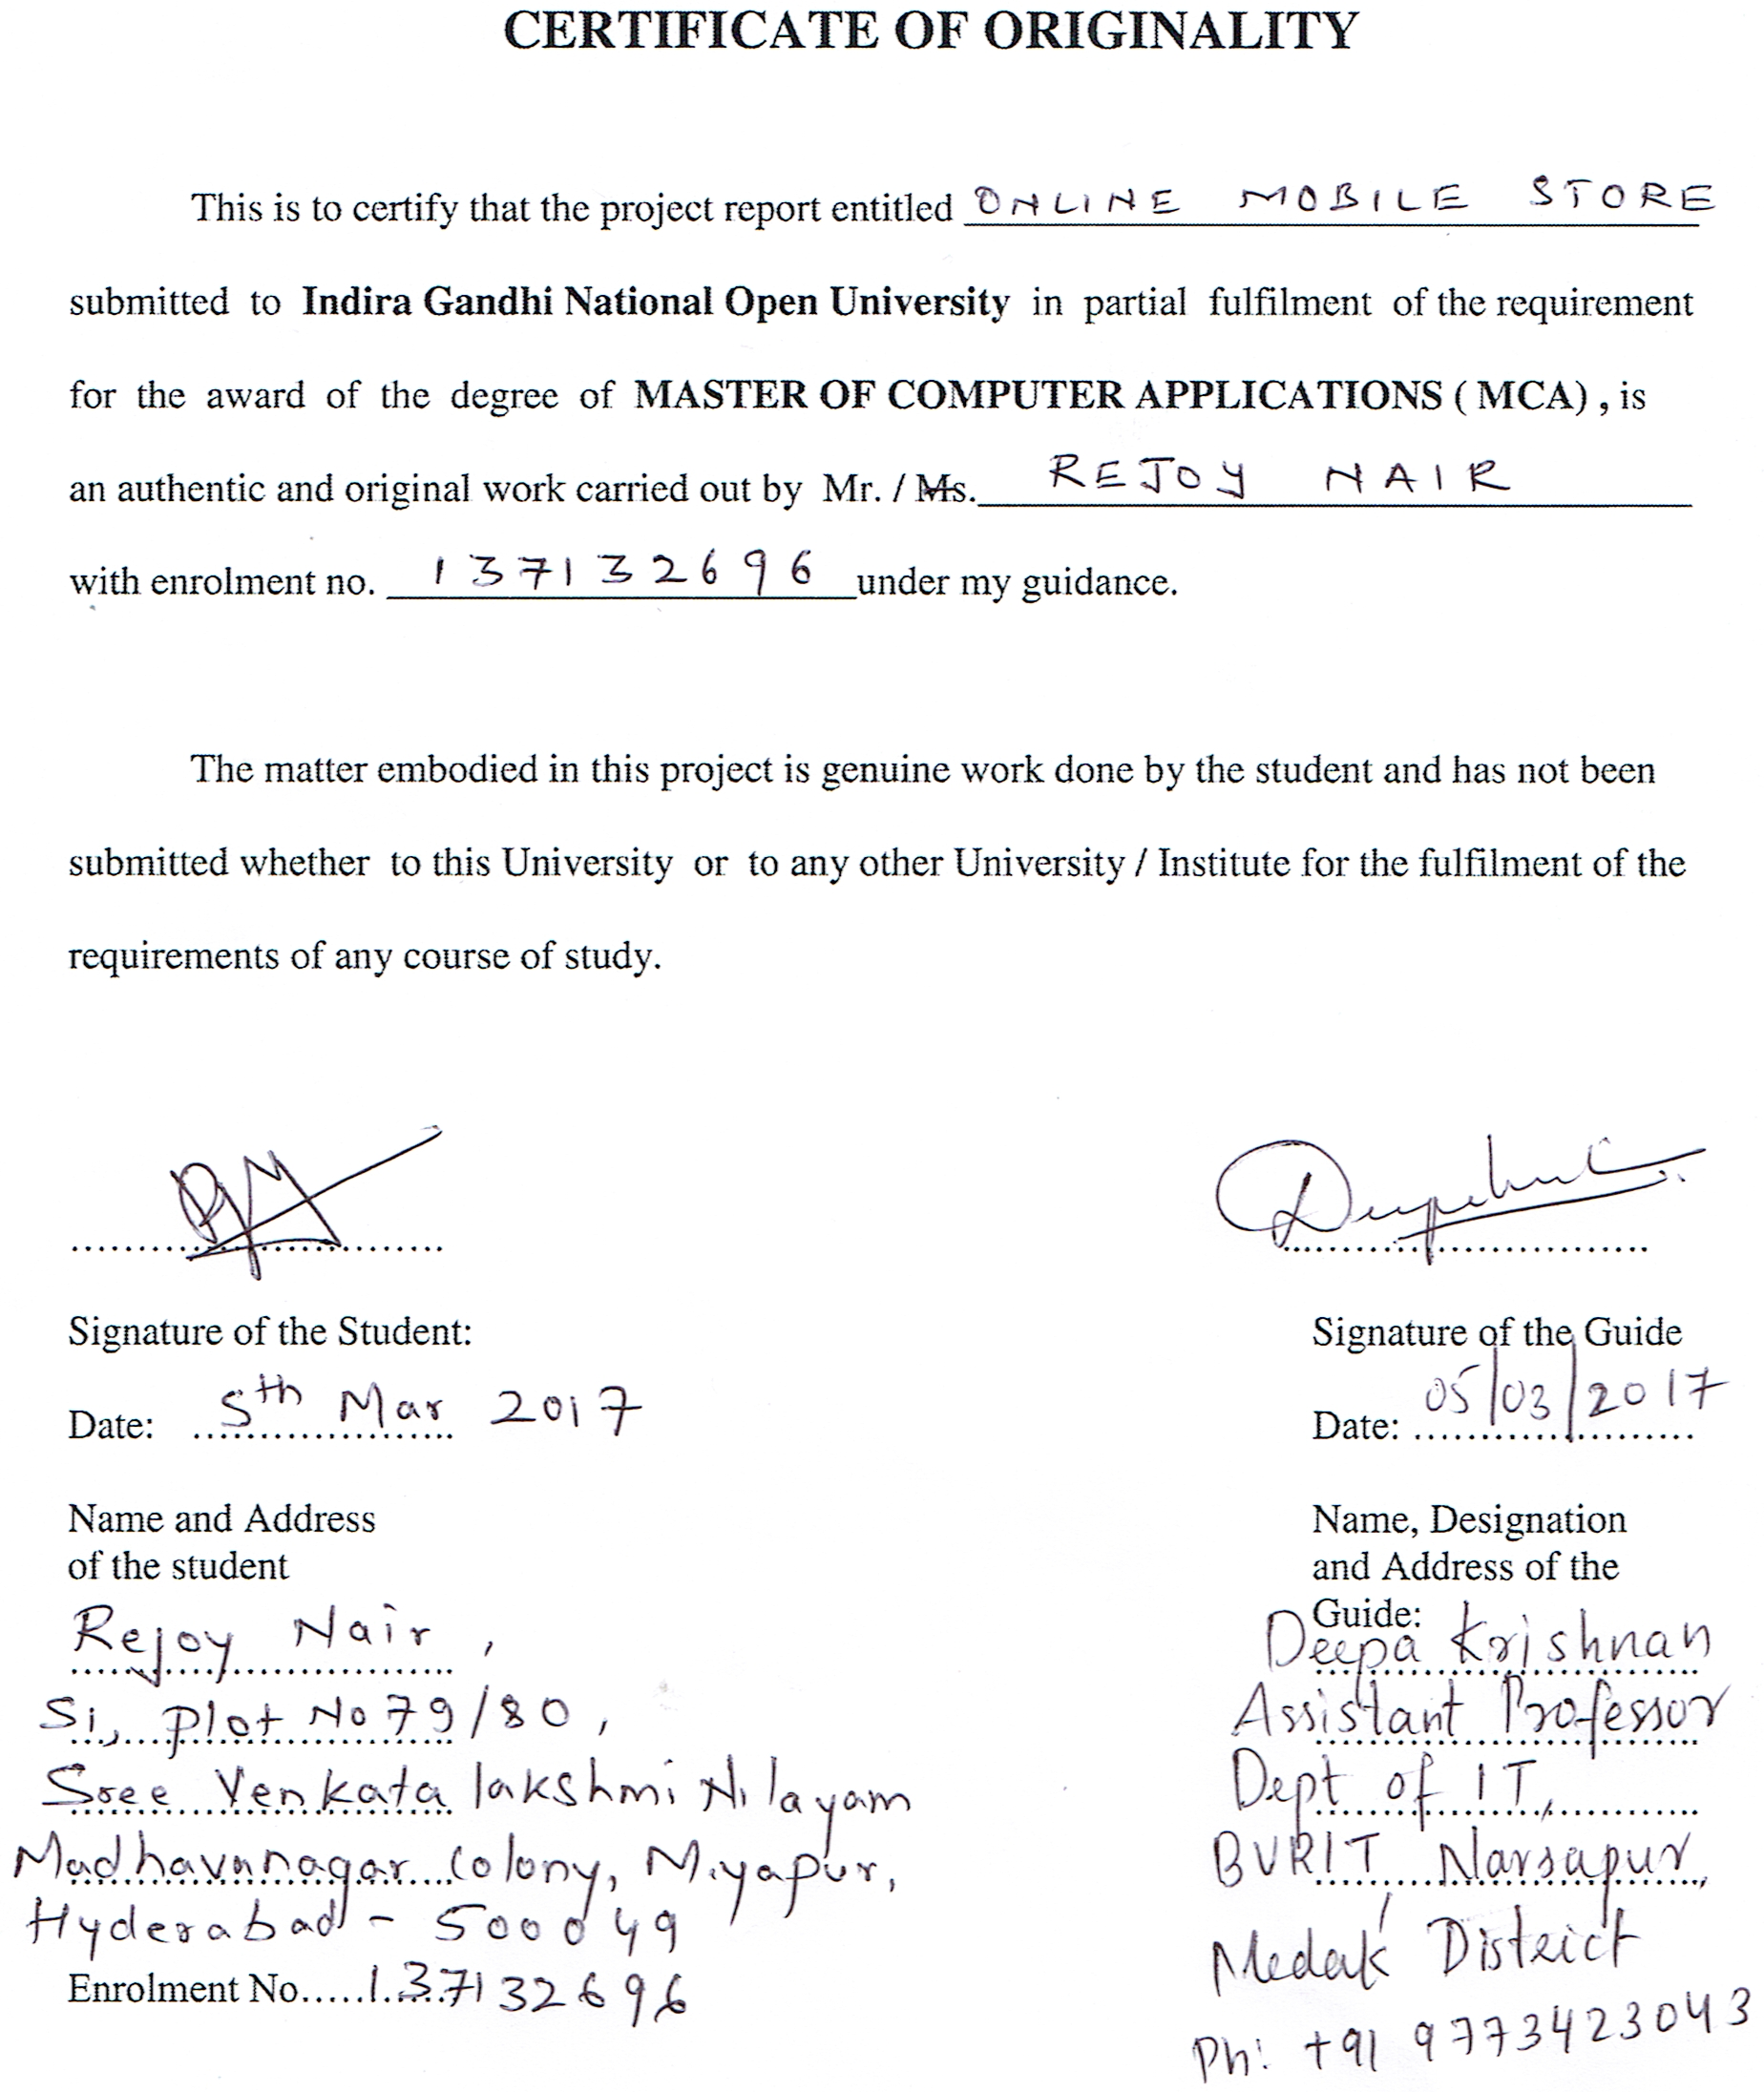
\includegraphics[ width= 0.76\paperwidth , keepaspectratio ]{./Images/CoOFilled.png}
\end{center}
\newpage

\tableofcontents

\setcounter{tocdepth}{3}	

\newpage

\clearpage

\pagestyle{plain}
%\pagestyle{fancy} 
\setcounter{page}{1}
%\fancyfoot[R]{\thepage}
\pagenumbering{arabic}
%\renewcommand{\thepage}{\roman{page}}

%*******************************************SECTION*******************************************************

\section{\MakeUppercase{Introduction / Objectives}}

\Gls{Electronic Commerce} commonly written as E-commerce or ecommerce is the trading or facilitation of trading using \gls{computer network} such as \Gls{Internet} or \Gls{Social Networks}. E-commerce draws on technologies like \Gls{mobile commerce}, Electronics Funds Transfer, \Gls{Supply Chain Management}, \Gls{Internet Marketing}, \Gls{Online Transaction Processing}, \Gls{EDI}, \Gls{Inventory Management} Systems and automated data collection systems. Modern electronic commerce typically uses the \Gls{World Wide Web} for at least one part of the transaction`s life cycle though it may also use other technologies like \gls{email}.
\\

Online Shopping is a form of electronic commerce which allows consumers to directly buy goods and services from a seller over the Internet using a \gls{web browser}. Consumers find a product of interest by visiting the website of the retailer directly or by searching among alternative vendors using a shopping \gls{search engine} which displays the same product`s availability and pricing at different vendors. Customers can shop online using a range of different computers and devices including desktop computers, laptops, tablet computers and smart-phones.

\subsection{Background}

An online shop evokes the physical analogy of buying products and services at regular ``bricks-and-mortar`` retailer or shopping center; the process is called \Gls{B2C} online shopping. A typical online store enables the customer to browse the firm`s range of products and services, view photos or images of the product along with the information about the product specification, features and prices.
\\

Online stores typically enable shoppers to use ``search`` features to find specific models, Brands or Items. Online customers must have valid access to the Internet and a valid method of payment in order to complete a transaction, such as a credit card, an Interac-enabled debit card, or a service such as \Gls{Paypal}. For physical products (e.g., paperback books or clothes), the e-tailer ships the products to the customer; for digital products, such as digital audio files of songs or software, the e-tailer typically sends the file to the customer over the Internet. The largest of these online retailing corporations are Alibaba, Amazon.com and eBay.
\\

English entrepreneur Michael Aldrich was a pioneer of online shopping in 1979\textsuperscript{[1]}. His system connected a modified domestic TV to a \gls{real-time transaction processing} computer  via a domestic telephone line. The first World Wide Web server and browser, created by Tim Berners-Lee in 1990, opened for commercial use in 1991. Thereafter, subsequent technological innovations emerged in 1994: online banking, the opening of an online pizza shop by Pizza Hut, Netscape \Gls{SSL} v2 encryption standard for secure data transfer and Intershop`s first  Online shopping system. The first retail transaction over the Web was either by NetMarket or Internet Shopping Network in 1994. Immediately after, Amazon.com launched its online shopping site in 1995 and eBay was also introduced in 1995. Alibaba`s sites Taobao and Tmall were launched in 2003 and 2003 respectively.
\\

\noindent
Mobile Phone online buying platforms can be broadly classified into 2 types

\begin{easylist}
& \thinspace Owned by Retailer to sell own products
& \thinspace \Gls{Marketplace}, which allows various merchants to showcase and sell their products. The retailer only manages the marketplace.
\end{easylist}
\bigskip
\noindent

This project describes a minimal implementation of a platform which the retailer can use to sell own products i.e. the retailer is accountable and responsible for the product inventory.

\subsection{Purpose \& Motivation}

The main purpose of this project is to create an online store to buy mobile phones. The site will allow users to search mobile phones from the products listing page. Users can add selected products to a shopping cart and checkout by making payment. Users will receive an order copy of their invoice.
\\

The retailer website will be managed by an Admin. Admin will have additional functionality such as managing product catalog and generating reports.
\\

\noindent
Motivation to work on this project includes
\begin{easylist}
& \thinspace Working on a project in the Retail domain
& \thinspace To gain knowledge of the working of a good user friendly website that facilitates online transactions using a database
& \thinspace Interest in technologies such as Golang, Javascript, HTML, CSS and SQL for web development
& \thinspace Explore data analytics that can be implemented using Golang
\end{easylist}
\bigskip
\noindent

\subsection{Objectives}

The Key objectives of the Project include
\begin{easylist}
& \thinspace Implementation of an Admin module for managing a website facilitating buying of mobile phones using online transactions.
& \thinspace Develop and host a website which allows users to search and explore mobile phones
& \thinspace Implement the shopping cart feature for the site that allows users to add selected products and tag it to a single order
& \thinspace Implement the online payment module (Credit Cards Only)
& \thinspace Explore technologies such as Golang, Javascript, HTML, CSS and SQL for web development
& \thinspace Explore data analytics that can be implemented using Golang
\end{easylist}

\subsection{Project Category}

This project can be categorized as a web development project that uses concepts of Internet technologies and \gls{web design}, \gls{web security} and \Gls{RDBMS}. Though Golang is not an \Gls{OOP} language, OOP has been achieved by making use of interfaces allowed in Golang. \Gls{Network security} has also been implemented for the website using \Gls{TLS}

\newpage

%*******************************************SECTION******************************************************

\section{\MakeUppercase{System Analysis}}

\subsection{Identification of Need}

Small scale retailers or start-up retailers in the mobile phone category would like to get their website up and running with a minimum investment in hardware and technology. The technology should be chosen in a way that allows to scale up later if required.
\\

Large retailers may want to look at alternative technologies that make possible to lower development time and cost translating to better Project Management and increased efficiency.
\\

Mobile Phones is an indicative category. The Online selling platform can be deployed for the purpose of selling almost any kind of product categories and services online. Mobile Phone Category has been chosen for this project due to the limited and universally well-understood feature set of the products of this category that allows to describe the project implementation without delving too much into the business aspects of the products.
\\

\subsection{Preliminary Investigation}

India was one of the fastest growing retail e-commerce markets in 2015, growing at the rate of 129.5 per cent Y-o-Y.  Declining \gls{broadband} subscription prices and the launch of \Gls{4G} services has become the driving forces of \gls{e-commerce} in the country. India will see more people come online than any other country in the next 15 years. With the penetration of digital devices and \gls{social media} in the interiors of the country, online sellers have been presented with an unprecedented opportunity of growth, becoming extremely attractive to investors. E-commerce is expected to acquire 4.8\% market share in total retail sales by 2019.
\\

Among e-tail categories, mobile phone and mobile accessories continue to be the top contributor to the overall pie\textsuperscript{[2]}. Retailers would be willing to invest in technology and even maintain it in-house provided it is low-cost, easy to maintain and of course effective in serving their business needs. This allows retailers to manage their own product catalog, respond to market dynamics by carrying out promotional campaigns, manage the look and feel of their website and quickly \gls{go-live} and roll-out the changes. Though all of this could also be achieved through an intermediate service provider, the retailer in that case would not be able to manage costs and time as they would like to.


\subsection{Feasibility Study}

The objective of a feasibility study is not to solve the problem but to acquire a sense of its scope. This project does not aim to build a full scale website that is ready for industrial deployment. The project aims to explore web development using Golang by creation of an online mobile store. The full scale implementation of the project is constrained by time, resource and cost and is in fact not really necessary for an academic project of this kind.
\\

The scope of the project shall be limited to
\begin{easylist}
& \thinspace User Registration and Sign-on
& \thinspace Manage Products Catalog
& \thinspace Order Management
&& Shopping Cart
&& Place Order
&& Cancel Order
& \thinspace Payment Gateway Integration
& \thinspace Notifications
& \thinspace Analytics \& Reports
\end{easylist}
\bigskip

\noindent
To deploy a website with the basic benchmarks as stated above the following tools, platforms, hardware and software were used.
\\

The development environment was set up on a \gls{i686} computer loaded with a 32-bit \Gls{Linux} operating system. The host environment shall be the same \gls{i686} computer with the 32-bit \Gls{Linux} operating system i.e., the development server and the host server are one and the same machine.
\\

Later, after the development process is complete, the option of deploying the web app on a remote host or Google App Engine may be explored for demo purpose.

\bigskip

\noindent
\begin{center}
	{
	\setlength{\extrarowheight}{2pt}

	\newcolumntype{b}{X}
	\newcolumntype{s}{>{\hsize=.4\hsize}X}
	\newcolumntype{t}{>{\hsize=1.3\hsize}X}
		
	%\renewcommand\thetable{2} 					
	%\caption{table}{ \textbf {\small {Software \& Hardware Requirements}}} \\ %\label{table:1}
	\vspace{0.25cm}
									
	\begin{tabularx}{\textwidth}{ | >{\ttfamily\raggedright\arraybackslash} s 
	| >{\ttfamily\raggedright\arraybackslash} t 
	| >{\ttfamily\raggedright\arraybackslash} t | }
								
	\caption{ \textbf {\small {Software \& Hardware Requirements}}} \\

	\hline
								
	{\textbf{\textcolor{black}{{Sr. No.} \newline}}} & {\textbf{\textcolor{black}{ {Tools \& Technologies}}}} & \textbf{\textcolor{black}{ {Description}}} \\
								
	\hline
	1.0 & Go ver 1.7 linux/386 & Tool for managing Go source code.Go (also commonly referred to as golang) is an open source systems programming language developed at Google  \\
	\hline		
	2.0 & net/http package & Package http of Golang that provides http client and server implementations  \\
	\hline
	3.0 & SQLite3 Database & SQLite is a self-contained high-reliability, full-featured, public-domain, SQL database engine.  \\ [1em]
	\hline
	4.0 & SQLite Manager & SQLite Manager is a Database Management System for SQLite database and is available as a firefox addon that can be used in the browser.  \\  [1em]
	\hline	  
	5.0 & Emacs ver. 24.3 & Development Environment  \\ 
	\hline	
	6.0 & go-mode & Emacs package for GoLang \\ [1em]
	\hline	
	7.0 & Geany ver 1.22 & A lightweight IDE with support for HTML, CSS, Javascript and JQuery \\ [1em]
	\hline	 
	8.0 & Github & Repository Management Cloud  \\ [1em]
	\hline	  
	9.0 & Git & Version Control System  \\ [1em]
	\hline
	10.0 & HTML5 & HTML 5 is the markup language used for structuring and designing content on the world wide web  \\ [1em]
	\hline	
	11.0 & CSS & A declarative stylesheet language for structured documents  \\ [1em]
	\hline	
	12.0 & Javascript & Javascript is a high-level, dynamic, untyped and interpreted programming language for front-end web functionality  \\ [1em]
	\hline
	13.0 & JQuery ver 1.11.3 & JQuery is a cross-platform javascript library designed to simplify the client side scripting of HTML  \\ [1em]
	\hline			    	    		    
	14.0 & Crunchbang Linux Waldorf 11.0 & \Gls{Operating System}   \\ 
	\hline	    
	15.0 & stripe-go & Golang package for Stripe \gls{API}. Stripe is a \Gls{Payment Gateway} Service provider   \\ 
	\hline	   	    		       	           								
	\end{tabularx}
	}
\end{center}
						
\bigskip
\noindent


\subsection{Project Planning}

\textbf{Software Development}

\begin{easylist}
& \thinspace The online Mobile Store shall be a minimalist functional website with functionalities as described in the scope
& \thinspace Server Code shall be developed entirely using Golang
& \thinspace \Gls{Web server} provided by Golang's ``net/http`` package shall be used to serve the pages
& \thinspace Front-end development shall be done using HTML 5, CSS3, Javascript and JQuery.
& \thinspace Shopping cart shall be developed entirely using javascript. The shopping cart will not be persistent and will be valid only for the User Session.
& \thinspace Stripe Checkout shall be used for \Gls{Payment Gateway}. \Gls{API} integration shall be done with the Go code.
& \thinspace \Gls{PSP} Software Development Methodology shall be followed 
\end{easylist}
\bigskip
\noindent


\textbf{Deployment \& \Gls{Hosting}}

\begin{easylist}
& \thinspace The website shall be hosted on the local server on which the development is done. Internet connectivity will be required for the web application to work
& \thinspace Options to deploy the web app on Google Cloud App Engine shall be explored for demo purpose
\end{easylist}
\bigskip
\noindent

\textbf{Testing}

\begin{easylist}
& \thinspace Test Scenarios, Test Cases \& Testing 
\end{easylist}
\bigskip
\noindent

\textbf{Resources \& Cost}

\begin{easylist}
& \thinspace This is an academic project and a single resource i.e., I myself shall be working on all aspects of the Project.
& \thinspace There is no financial cost attributed to the project other than the renumeration bill for the Project Guide to be footed by IGNOU.
\end{easylist}
\bigskip
\noindent

\subsection{Project Scheduling}

\noindent

\textbf{Major deliverables of this project are:}

\begin{easylist}
& \thinspace Setting up the development environment
& \thinspace Code implementation of key functions i.e Product Catalouge, Sign-On, Order management \& Reports
& \thinspace Payment API Integration
& \thinspace Test Scenarios, Test Cases \& Testing 
& \thinspace Deployment \& Hosting
\end{easylist}
\bigskip

\begin{sideways}
\centering
\begin{minipage}{\textheight}
\begin{center}
			
		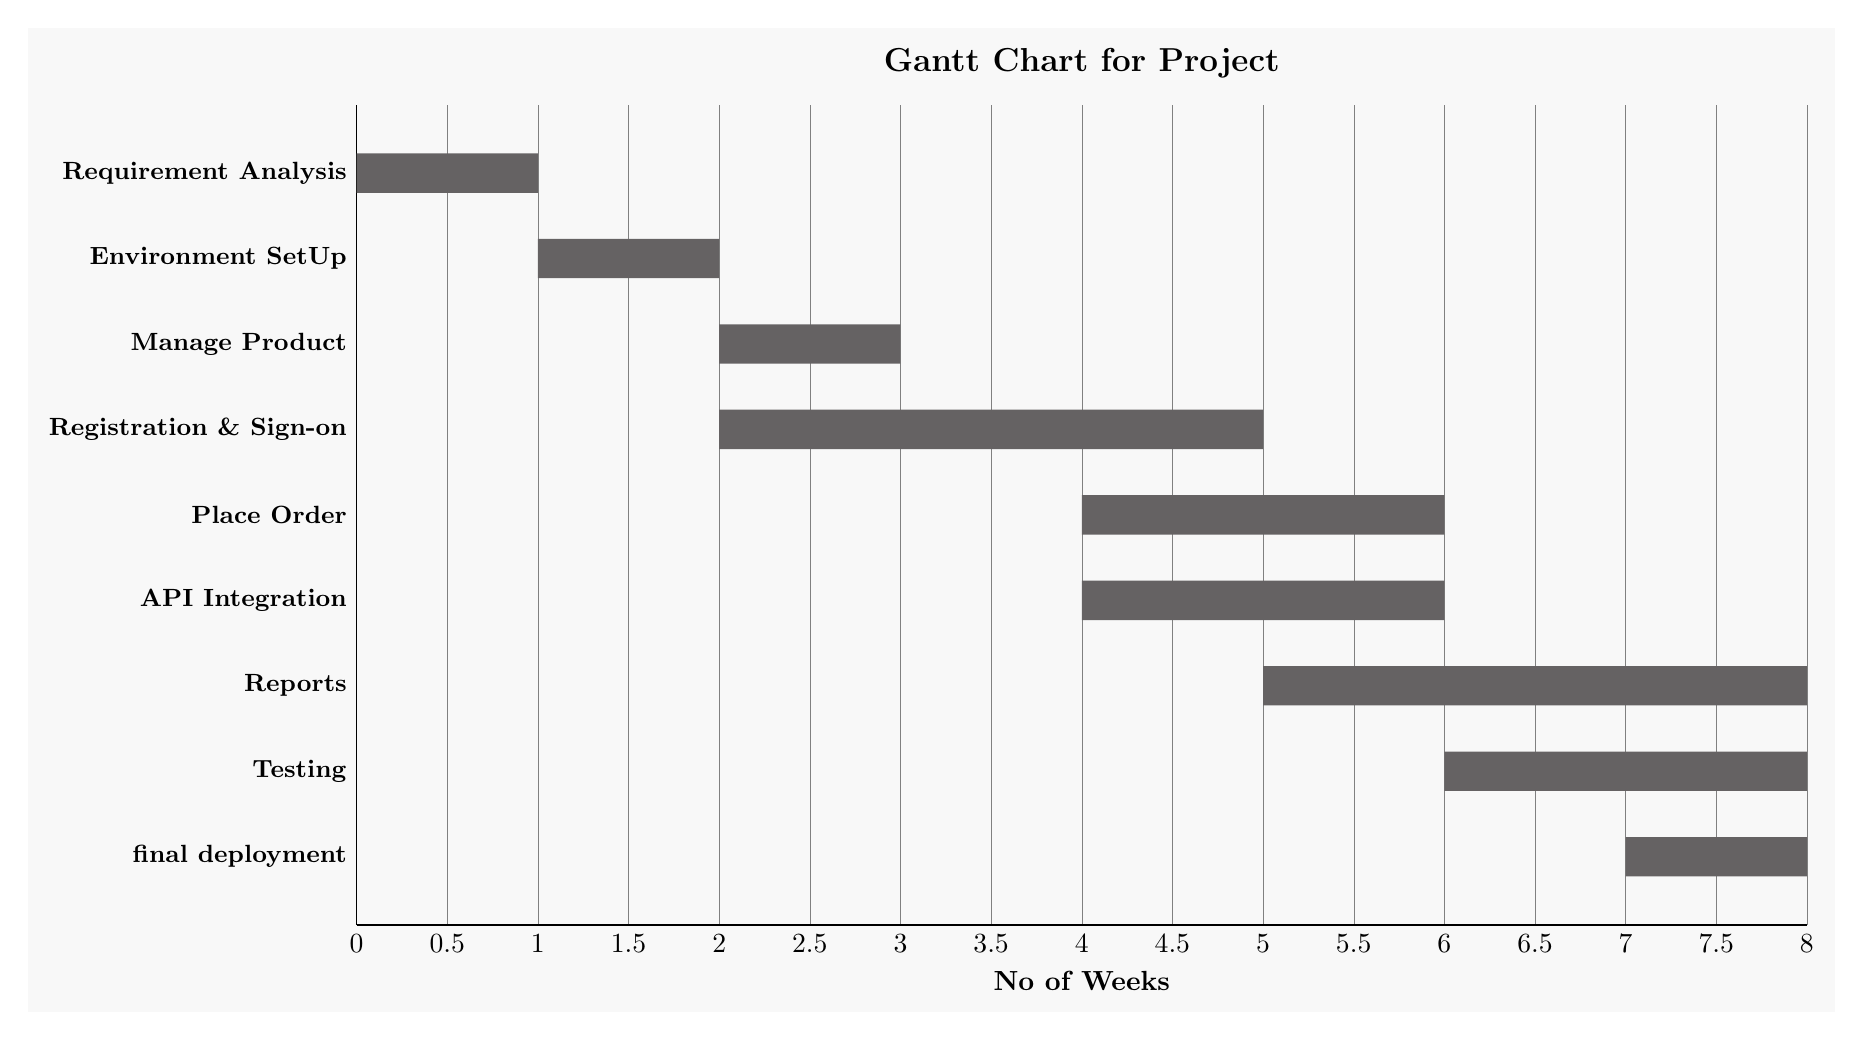
\begin{tikzpicture}[use background]
		
		\pgfplotstableread{ % Read the data into a table macro
			Label                                                      First   Second  
			{\small \textbf{final deployment}}                           7     1
			{\small \textbf{Testing}}                                    6     2
			{\small \textbf{Reports}}                                    5     3
			{\small \textbf{API Integration }}                           4     2
			{\small \textbf{Place Order}}                                4     2
			{\small \textbf{Registration \& Sign-on}}                    2     3
			{\small \textbf{Manage Product}}                             2     1
			{\small \textbf{Environment SetUp}}                          1     1
			{\small \textbf{Requirement Analysis}}                       0     1
		}\datatable
		
		\begin{axis}[
		xbar stacked,   % Stacked horizontal bars
		xmin=0,  xmax=8,       % Start x axis at 0
		title={\large \textbf {Gantt Chart for Project}},
		height=12cm, width=20cm,
		bar width=0.5cm,
		axis x line*=bottom,
		axis y line*=left,
		y axis line style={opacity=1},
		enlarge y limits=true,
		xmajorgrids={true},
		grid style={
			solid,
			ultra thin,
			gray
		},
		tick style={tickwidth=0cm,major tick length=0cm},
		xlabel={\textbf{No of Weeks }},
		ytick=data,     % Use as many tick labels as y coordinates
		yticklabels from table={\datatable}{Label}  % Get the labels from the Label column of the \datatable
		]
		\addplot [draw=none,fill=none] table [x=First, y expr=\coordindex] {\datatable};    % Plot the "First" column against the data index
		\addplot [draw=none,fill={levelfirst}]table [x=Second, y expr=\coordindex] {\datatable};
		
		
		\end{axis}
		
		\end{tikzpicture}
		
\end{center}
\end{minipage}
\end{sideways}


\subsection{\Gls{Software Requirement Specifications}}

\subsubsection{Problem Definition}
Mobile Phone Retailer requires to present inventory to customers online and facilitate users to search, select and place orders for mobile phones as well as make payments online.
Retailer should be able to manage the platform that allows the buying of mobile phones online.

\subsubsection{User Module}
Users can register, login, search for products, add selected products to shopping cart and place orders after check-out

\subsubsection{User Module - Registration}
Users can register on the customer website by clicking on a link that directs them to the Sign-up or registration form. Users have to provide the username with which they register, first and last name, an email address and confirm the password they want to create for the username

\begin{center}
	{
	\setlength{\extrarowheight}{2pt}

	\newcolumntype{b}{X}
	\newcolumntype{s}{>{\hsize=.4\hsize}X}
	\newcolumntype{t}{>{\hsize=0.9\hsize}X}
		
	%\renewcommand\thetable{2} 					
	%\caption{table}{ \textbf {\small {Requirements - User Module - Registration}}} \\ %\label{table:2}
	\vspace{0.25cm}
									
	\begin{tabularx}{\textwidth}{ | >{\ttfamily\raggedright\arraybackslash} s 
	| >{\ttfamily\raggedright\arraybackslash} t 
	| >{\ttfamily\raggedright\arraybackslash} t 	
	| >{\ttfamily\raggedright\arraybackslash} t | }
								
	\caption{ \textbf {\small {Requirements - User Module - Registration}}} \\
	
	\hline
								
	{\textbf{\textcolor{black}{ {Req. ID} \newline}}} & {\textbf{\textcolor{black}{ { Description}}}} & {\textbf{\textcolor{black}{ {UI Element \& Datatype}}}} & \textbf{\textcolor{black}{ {Validation}}} \\
								
	\hline
	\newFR\label{Signup:1}  & User should be able to navigate to the sign-up / registration form from the landing page & Hyperlink & User should have a secure connection to the website \\
	\hline	
	\newFR\label{Signup:2} & User should be able to create a unique username for registration purpose &  Input text box \newline \newline String & should be unique \newline \newline should be alphanumeric \\
	\hline		
	\newFR\label{Signup:3} & User should be able to create a provide First Name, Last name and email address for registration purpose. Email address should be unique &  Input text boxes \newline \newline String & Should be string (alpha) \newline \newline Email Address should be a valid email ID and unique \\
	\hline		
	\newFR\label{Signup:4} & User should be able to create a create a password for the username &  Password box \newline \newline string & should be alphanumerc \newline \newline User is required to reconfirm \\
	\hline
	\newFR\label{Signup:5} & User should receive error alerts for invalid input &  Alert boxes \newline \newline String & Empty space is not allowed \newline Fields that require unique value shall only accept such values \newline \newline Fields not meeting the criteria described in the regex pattern for the field shall be invalidated \\	
	\hline	   	    		       	           								
	\end{tabularx}
	}
\end{center}
						
\newpage

\subsubsection{User Module - Sign-On}
User can sign-on using the username and password

\begin{center}
	{
	\setlength{\extrarowheight}{2pt}

	\newcolumntype{b}{X}
	\newcolumntype{s}{>{\hsize=.4\hsize}X}
	\newcolumntype{t}{>{\hsize=0.9\hsize}X}
		
	%\renewcommand\thetable{2} 					
	%\caption{table}{ \textbf {\small {Requirements - User Module - Registration}}} \\ %\label{table:3}
	\vspace{0.25cm}
									
	\begin{tabularx}{\textwidth}{ | >{\ttfamily\raggedright\arraybackslash} s 
	| >{\ttfamily\raggedright\arraybackslash} t 
	| >{\ttfamily\raggedright\arraybackslash} t 	
	| >{\ttfamily\raggedright\arraybackslash} t | }
								
	\caption{ \textbf {\small {Requirements - User Module - Registration}}} \\
	
	\hline
								
	{\textbf{\textcolor{black}{ {Req. ID} \newline}}} & {\textbf{\textcolor{black}{ { Description}}}} & {\textbf{\textcolor{black}{ {UI Element \& Datatype}}}} & \textbf{\textcolor{black}{ {Validation}}} \\
								
	\hline
	\newFR\label{login:1}  & User connection should be secure  &   & Transport Layer Security (TLS) should be implemented \newline \newline Secure connection via \Gls{HTTPS} \\
	\hline	
	\newFR\label{login:2} & User should be able to log into the website using the username and password created at the time of registration &  Input text boxes \newline \newline String & User should \gls{authenticate} by providing valid password \newline \newline New \gls{session} shall be generated for every successful login \\
	\hline		
	\newFR\label{login:3} & User should receive error alerts for invalid input &  Alert boxes \newline \newline string & Username cannot be empty and should be valid \newline \newline Password should correspond to the correct password of the username maintained at the server. \\
	\hline	
	\end{tabularx}
	}
\end{center}
						
\bigskip
\noindent


\subsubsection{User Module - Search Products}
User can search for specific products in the product catalog by description. By default all products shall be listed in the main view.


\begin{center}
	{
	\setlength{\extrarowheight}{2pt}

	\newcolumntype{b}{X}
	\newcolumntype{s}{>{\hsize=.4\hsize}X}
	\newcolumntype{t}{>{\hsize=0.9\hsize}X}
		
	%\renewcommand\thetable{2} 					
	%\caption{table}{ \textbf {\small {Requirements - User Module - Product Listing \& Search}}} \\ %\label{table:4}
	\vspace{0.25cm}
									
	\begin{tabularx}{\textwidth}{ | >{\ttfamily\raggedright\arraybackslash} s 
	| >{\ttfamily\raggedright\arraybackslash} t 
	| >{\ttfamily\raggedright\arraybackslash} t 	
	| >{\ttfamily\raggedright\arraybackslash} t | }
								
	\caption{ \textbf {\small {Requirements - User Module - Product Listing \& Search}}} \\

	\hline
								
	{\textbf{\textcolor{black}{ {Req. ID} \newline}}} & {\textbf{\textcolor{black}{ { Description}}}} & {\textbf{\textcolor{black}{ {UI Element \& Datatype}}}} & \textbf{\textcolor{black}{ {Validation}}} \\
								
	\hline
	\newFR\label{Prodlist:1}  & All products should be listed in the main view. Listings should include the image, name and price of the product &  Info Panel \newline \newline Image File, String & data object should be present in the product catalog \\
	\hline	
	\newFR\label{Prodlist:2} & User should be able to search the product by entering string that shall be matched with the product description. User should be able to view only such products that fulfill the search criteria &  Search Box \newline \newline string & Search string cannot be empty \\
	\hline		
	\newFR\label{Prodlist:3} & User should be able to select a product by adding it to the shopping cart &  Button \newline \newline Each product info panel shall have its own button  & A single unit of the product shall be added to the shopping cart each time the button is clicked \\
	\hline									
	\end{tabularx}
	}
\end{center}
						
\bigskip
\noindent

\subsubsection{Shopping Cart}
Selected products can be added to shopping cart. Shopping Cart is not \gls{persistent} i.e. it is valid only for the session.

\begin{center}
	{
	\setlength{\extrarowheight}{2pt}

	\newcolumntype{b}{X}
	\newcolumntype{s}{>{\hsize=.4\hsize}X}
	\newcolumntype{t}{>{\hsize=0.9\hsize}X}
		
	%\renewcommand\thetable{2} 					
	%\caption{table}{ \textbf {\small {Requirements - User Module - Shopping Cart}}} \\ %\label{table:5}
	\vspace{0.25cm}
									
	\begin{tabularx}{\textwidth}{ | >{\ttfamily\raggedright\arraybackslash} s 
	| >{\ttfamily\raggedright\arraybackslash} t 
	| >{\ttfamily\raggedright\arraybackslash} t 	
	| >{\ttfamily\raggedright\arraybackslash} t | }
	
	\caption{ \textbf {\small {Requirements - User Module - Shopping Cart}}} \\
								
	\hline
								
	{\textbf{\textcolor{black}{ {Req. ID} \newline}}} & {\textbf{\textcolor{black}{ { Description}}}} & {\textbf{\textcolor{black}{ {UI Element \& Datatype}}}} & \textbf{\textcolor{black}{ {Validation}}} \\
								
	\hline
	\newFR\label{Shcart:1}  & User should be able to view the list of products added to the shopping cart. The list should include the image, name and price of the product. &  Dropdown list (Tabular) \newline \newline image File, String & Details of the Product should be similar to the selected product in all aspects \\
	\hline	
	\newFR\label{Shcart:2} & User should be able to change the quantity of the product added to the shopping cart &  Input Number Box \newline \newline Integer & Minimum value shall be 1 \\
	\hline		
	\newFR\label{Shcart:3} & User should be able to view the total cost per product in the shopping cart &  Output text \newline \newline Number & Total Cost cannot be Zero \newline \newline Total Cost = Quantity * Price Per Unit \\
	\hline	
	\newFR\label{Shcart:4} & User should be remove the product from the shopping cart &  Button & Quantity should be decremented by 1 each time this button is clicked \newline \newline Entire line item should get removed if the product quantity is 1 when this button gets clicked. i.e., it is equivalent to removing the product from the shopping cart \\
	\hline	
	\newFR\label{Shcart:5} & User should be able to checkout and directly place an order from the shopping cart &  Button & User session should be valid \\
	\hline										
	\end{tabularx}
	}
\end{center}

\newpage
\subsubsection{Place Order}
Users can trigger orders after checkout by making payment.

\begin{center}
	{
	\setlength{\extrarowheight}{2pt}

	\newcolumntype{b}{X}
	\newcolumntype{s}{>{\hsize=.4\hsize}X}
	\newcolumntype{t}{>{\hsize=0.9\hsize}X}
		
	%\renewcommand\thetable{2} 					
	%\caption{table}{ \textbf {\small {Requirements - User Module - Place Order}}} \\ %\label{table:6}
	\vspace{0.25cm}
									
	\begin{tabularx}{\textwidth}{ | >{\ttfamily\raggedright\arraybackslash} s 
	| >{\ttfamily\raggedright\arraybackslash} t 
	| >{\ttfamily\raggedright\arraybackslash} t 	
	| >{\ttfamily\raggedright\arraybackslash} t | }
	
	\caption{ \textbf {\small {Requirements - User Module - Place Order}}} \\
								
	\hline
								
	{\textbf{\textcolor{black}{ {Req. ID} \newline}}} & {\textbf{\textcolor{black}{ { Description}}}} & {\textbf{\textcolor{black}{ {UI Element \& Datatype}}}} & \textbf{\textcolor{black}{ {Validation}}} \\
								
	\hline
	\newFR\label{Plcord:1}  & User should be able to view the list of products in the order basket. The list should include the image, name, quantity and price of the product. &  Order Data info panel \newline \newline Image file, String, Integer & List of products should correspond to the ones added to the shopping cart \newline \newline Product details must be equal in all respects to the ones added to the shopping cart \\
	\hline	
	\newFR\label{Plcord:2} & User should be able to view the total cost per product in the order basket &  Output Text \newline \newline Number & Total Cost cannot be Zero \newline \newline Total Cost = Quantity * Price Per Unit \\
	\hline		
	\newFR\label{Plcord:3} & User should be able to view the overall order quantity of products and the overall order cost &  Output Text \newline \newline Integer, Number & Overall Order Quantity cannot be Zero. \newline \newline Overall order cost cannot be zero. \newline \newline Overall Order Quantity = Sum of total quantity of individual product items of the order basket \newline \newline Overall Total Cost = Sum of total cost of individual product items of the order basket \\
	\hline	
	\newFR\label{Plcord:4} & User should be able to initiate payment for the order &  Button & User session should be valid \\
	\hline	
	\newFR\label{Plcord:5} & User should be able to navigate back to the product listings page &  Link & User session should be valid \\
	\hline										
	\end{tabularx}
	}
\end{center}

\newpage
\subsubsection{User Module - Make Payment}
Users can use the \gls{Payment Gateway} integrated into the website using \gls{API}.

\begin{center}
	{
	\setlength{\extrarowheight}{2pt}

	\newcolumntype{b}{X}
	\newcolumntype{s}{>{\hsize=.4\hsize}X}
	\newcolumntype{t}{>{\hsize=0.9\hsize}X}
		
	%\renewcommand\thetable{2} 					
	%\captionof{table}{ \textbf {\small {Requirements - User Module - Make Payment}}} \label{table:2}
	\vspace{0.25cm}
									
	\begin{tabularx}{\textwidth}{ | >{\ttfamily\raggedright\arraybackslash} s 
	| >{\ttfamily\raggedright\arraybackslash} t 
	| >{\ttfamily\raggedright\arraybackslash} t 	
	| >{\ttfamily\raggedright\arraybackslash} t | }
								
	\caption{ \textbf {\small {Requirements - User Module - Make Payment}}} \\
	
	\hline
								
	{\textbf{\textcolor{black}{ {Req. ID} \newline}}} & {\textbf{\textcolor{black}{ { Description}}}} & {\textbf{\textcolor{black}{ {UI Element \& Datatype}}}} & \textbf{\textcolor{black}{ {Validation}}} \\
								
	\hline
	\newFR\label{Pay:1}  & User should be able to provide cardholder`s email address in the Stripe Payment form &  Input Text box \newline \newline String & email address field cannot be empty \newline \newline email address should be a valid email address \\
	\hline	
	\newFR\label{Pay:2} & User should be able to provide billing \& shipping address in the Stripe Payment form &  Input text boxes \newline Dropdown list \newline \newline String & Address line 1 field cannot be empty \newline \newline Pincode field cannot be empty \newline \newline Town / City field cannot be empty \newline \newline Country Field cannot be empty \\
	\hline		
	\newFR\label{Pay:3} & User should be able to provide card details i.e, the card number, card expiry date and CVV number in the Stripe Payment form & Input boxes \newline datetime widget \newline \newline Number  & Card Number field cannot be empty \newline \newline card expiry date cannot be blank or a previous date \newline \newline CVV Number field cannot be blank \\
	\hline	
	\newFR\label{Pay:4} & User should be able save input card details to the Stripe server &  Checkbox \newline \newline boolean & Card details should be filled out for the checkbox to get enabled \\
	\hline	
	\newFR\label{Pay:5} & User should be able to exit the Stripe payment form & Exit form button & User should be navigated to the make payment page \\
	\hline										
	\end{tabularx}
	}
\end{center}


\subsubsection{User Module - Invoice}
Users can receive invoice copy on their registered email addresses as well on the card-holder`s email address

\begin{center}
	{
	\setlength{\extrarowheight}{2pt}

	\newcolumntype{b}{X}
	\newcolumntype{s}{>{\hsize=.4\hsize}X}
	\newcolumntype{t}{>{\hsize=0.9\hsize}X}
		
	%\renewcommand\thetable{2} 					
	%\captionof{table}{ \textbf {\small {Requirements - User Module - Invoice}}} \label{table:2}
	\vspace{0.25cm}
									
	\begin{tabularx}{\textwidth}{ | >{\ttfamily\raggedright\arraybackslash} s 
	| >{\ttfamily\raggedright\arraybackslash} t 
	| >{\ttfamily\raggedright\arraybackslash} t 	
	| >{\ttfamily\raggedright\arraybackslash} t | }
								
	\caption{ \textbf {\small {Requirements - User Module - Invoice}}} \\
	
	\hline
								
	{\textbf{\textcolor{black}{ {Req. ID} \newline}}} & {\textbf{\textcolor{black}{ { Description}}}} & {\textbf{\textcolor{black}{ {UI Element \& Datatype}}}} & \textbf{\textcolor{black}{ {Validation}}} \\
								
	\hline
	\newFR\label{Inv:1}  & User should receive order invoice copy cum payment receipt upon a successful order placement &  Info Panel & User session should be valid \newline \newline Invoice copy cum payment receipt cannot be empty.  \\
	\hline	
	\newFR\label{Inv:2} & User should receive a unique order ID in the order invoice cum payment receipt for each new order placed. &  Output text \newline \newline String & should be unique \\
	\hline		
	\newFR\label{Inv:3} & The Order invoice cum payment receipt should contain details of the products ordered that include the image, name, quantity, price per unit and the total price of the product. &  Info Panel \newline \newline Image file, String & Products details in the Invoice copy cum payment receipt cannot be empty. \\
	\hline	
	\newFR\label{Inv:4} & The Order invoice cum payment receipt should contain the total quantity of products ordered and the total order value &  Output text \newline \newline Integer, Number & the total quantity of products ordered and the total order value in the Invoice copy cum payment receipt cannot be empty.  \\
	\hline	
	\newFR\label{Inv:5} & User should receive error alerts in case of a failed transaction &  Alert Message \newline \newline string & user session should be valid \\
	\hline										
	\end{tabularx}
	}
\end{center}

\newpage
\subsubsection{User Module - Notifications}
User can receive notifications regarding sign-in, selected products, payment success and order confirmation. 

\begin{center}
	{
	\setlength{\extrarowheight}{2pt}

	\newcolumntype{b}{X}
	\newcolumntype{s}{>{\hsize=.4\hsize}X}
	\newcolumntype{t}{>{\hsize=0.9\hsize}X}
		
	%\renewcommand\thetable{2} 					
	%\captionof{table}{ \textbf {\small {Requirements - User Module - Invoice}}} \label{table:2}
	\vspace{0.25cm}
									
	\begin{tabularx}{\textwidth}{ | >{\ttfamily\raggedright\arraybackslash} s 
	| >{\ttfamily\raggedright\arraybackslash} t 
	| >{\ttfamily\raggedright\arraybackslash} t 	
	| >{\ttfamily\raggedright\arraybackslash} t | }
	
	\caption{ \textbf {\small {Requirements - User Module - Invoice}}} \\
								
	\hline
								
	{\textbf{\textcolor{black}{ {Req. ID} \newline}}} & {\textbf{\textcolor{black}{ { Description}}}} & {\textbf{\textcolor{black}{ {UI Element \& Datatype}}}} & \textbf{\textcolor{black}{ {Validation}}} \\
								
	\hline
	\newFR\label{Em:1}  & User should receive email notification on successful order placement & Email message delivered to user inbox & Email notification shall be sent to the registered email address of the customer \newline \newline Email notification shall be sent to the email address of the cardholder making the payment \\
	\hline											
	\end{tabularx}
	}
\end{center}

\newpage

\subsubsection{Admin Module}
Administrator of the website can manage the product catalog and view order data

\subsubsection{Admin Module - View Order data}
Administrator user of the website should be able to view the orders being placed on the customer web portal

\begin{center}
	{
	\setlength{\extrarowheight}{2pt}

	\newcolumntype{b}{X}
	\newcolumntype{s}{>{\hsize=.4\hsize}X}
	\newcolumntype{t}{>{\hsize=0.9\hsize}X}
		
	%\renewcommand\thetable{2} 					
	%\captionof{table}{ \textbf {\small {Requirements - Admin Module - View Order Data}}} \label{table:2}
	\vspace{0.25cm}
									
	\begin{tabularx}{\textwidth}{ | >{\ttfamily\raggedright\arraybackslash} s 
	| >{\ttfamily\raggedright\arraybackslash} t 
	| >{\ttfamily\raggedright\arraybackslash} t 	
	| >{\ttfamily\raggedright\arraybackslash} t | }
	
	\caption{ \textbf {\small {Requirements - Admin Module - View Order Data}}} \\	
							
	\hline
								
	{\textbf{\textcolor{black}{ {Req. ID} \newline}}} & {\textbf{\textcolor{black}{ { Description}}}} & {\textbf{\textcolor{black}{ {UI Element \& Datatype}}}} & \textbf{\textcolor{black}{ {Validation}}} \\
								
	\hline
	\newFR\label{Vord:1}  & Admin user should be able to view order data i.e, Order ID, Order Amount and the Order timestamp &  Output text \newline \newline String & None of the fields can be invalid or empty \\
	\hline		
	\newFR\label{Vord:2}  & Admin user should be able to navigate to the Manage Products page &  link & Admin user session should be valid \\
	\hline											
	\end{tabularx}
	}
\end{center}

\newpage
\subsubsection{Admin Module - Manage Products}
Admin can create, edit and delete products maintained in the product catalog. User is presented with the list managed by Admin.

\begin{center}
	{
	\setlength{\extrarowheight}{2pt}

	\newcolumntype{b}{X}
	\newcolumntype{s}{>{\hsize=.4\hsize}X}
	\newcolumntype{t}{>{\hsize=0.9\hsize}X}
		
	%\renewcommand\thetable{2} 					
	%\captionof{table}{ \textbf {\small {Requirements - Admin Module - Manage Products}}} \label{table:2}
	\vspace{0.25cm}
									
	\begin{tabularx}{\textwidth}{ | >{\ttfamily\raggedright\arraybackslash} s 
	| >{\ttfamily\raggedright\arraybackslash} t 
	| >{\ttfamily\raggedright\arraybackslash} t 	
	| >{\ttfamily\raggedright\arraybackslash} t | }
	
	\caption{ \textbf {\small {Requirements - Admin Module - Manage Products}}} \\	
							
	\hline
								
	{\textbf{\textcolor{black}{ {Req. ID} \newline}}} & {\textbf{\textcolor{black}{ { Description}}}} & {\textbf{\textcolor{black}{ {UI Element \& Datatype}}}} & \textbf{\textcolor{black}{ {Validation}}} \\
								
	\hline
	\newFR\label{Mprod:1} & Admin user should be able to navigate to the `Add Product Form' by clicking a link or button &  Button & Admin user session should be valid \\
	\hline		
	\newFR\label{Mprod:2} & Admin user should be able to view the product details such as the image, name, quantity and price of the products in the product catalog &  Info table \newline \newline Image file, String & Product details should correspond to the ones maintained at the backend database \\
	\hline	
	\newFR\label{Mprod:3} & Admin user should be able to delete a product from the product catalog &  Button & Line item for the product should get removed from the table view \newline \newline Product should exist in the backend database for it to get removed \\
	\hline	
	\newFR\label{Mprod:4} & Admin user should be able to update a product of the product catalog by navigating to the `Update Product Catalog' form &  Button & Product details should be fetched from the backend database and should get displayed in the update Product Form \\
	\hline	
	\newFR\label{Mprod:5} & Admin user should be able to navigate to the Admin main view i.e. `View Order Data' &  link & Admin user session should be valid \\
	\hline													
	\end{tabularx}
	}
\end{center}

\subsubsection{Admin Module - Add Product}

\begin{center}
	{
	\setlength{\extrarowheight}{2pt}

	\newcolumntype{b}{X}
	\newcolumntype{s}{>{\hsize=.4\hsize}X}
	\newcolumntype{t}{>{\hsize=0.9\hsize}X}
		
	%\renewcommand\thetable{2} 					
	%\captionof{table}{ \textbf {\small {Requirements - Admin Module - Add Products}}} \label{table:2}
	\vspace{0.25cm}
									
	\begin{tabularx}{\textwidth}{ | >{\ttfamily\raggedright\arraybackslash} s 
	| >{\ttfamily\raggedright\arraybackslash} t 
	| >{\ttfamily\raggedright\arraybackslash} t 	
	| >{\ttfamily\raggedright\arraybackslash} t | }
	
	\caption{ \textbf {\small {Requirements - Admin Module - Add Products}}} \\		
						
	\hline
								
	{\textbf{\textcolor{black}{ {Req. ID} \newline}}} & {\textbf{\textcolor{black}{ { Description}}}} & {\textbf{\textcolor{black}{ {UI Element \& Datatype}}}} & \textbf{\textcolor{black}{ {Validation}}} \\
								
	\hline
	\newFR\label{Addprod:1} & Admin user should be able to create a product by adding a product name, product quantity,and image  &  Input Text boxes \newline File Upload utility \newline \newline String, Image file & Product name should be unique \newline \newline Image file name should be unique \newline \newline Image quantity cannot be zero \\
	\hline		
	\newFR\label{Addprod:2} & Admin user should be able upload an image for the product being added &  File Upload utility \newline \newline Image file & image file cannot be empty. \newline \newline Image filename cannot be empty and should be valid \\
	\hline	
	\newFR\label{Addprod:3} & A unique product ID should get generated for each new product created &  \Gls{UUID} \newline \newline \Gls{UUID} & Product ID should unique \\
	\hline	
	\newFR\label{Addprod:4} & Admin user should be able logoff, go back to the previous page, directly go to the Manage Product page or the View Order data page using links or buttons &  Link & Admin user session should be valid \\
	\hline	
	\newFR\label{Addprod:5} & Admin user should receive error alerts for invalid inputs &  Alert boxes \newline \newline string &  Empty space is not allowed \newline Fields that require unique value shall only accept such values \newline \newline Fields not meeting the criteria described in the regex pattern for the field shall be invalidated \\
	\hline													
	\end{tabularx}
	}
\end{center}


\subsubsection{Reports}
Admin can generate basic report of products purchased on the website.
\newpage

\subsection{Software Engineering Paradigm applied}

\subsubsection{The Personal Software Process (PSP)}

The \Gls{PSP} is a structured software development process that is intended (planned) to help software engineers better understand and improve their performance by tracking their predicted and actual development of code. The PSP was created by Watts Humphrey to apply the underlying principles of the Software Engineering Institute`s (SEI) \Gls{CMM} to the software development practices of a single developer. It claims to give software engineers the process skills necessary to work on a \Gls{TSP} team \textsuperscript{[3]}.
\\

\begin{figure}[H]
\centering
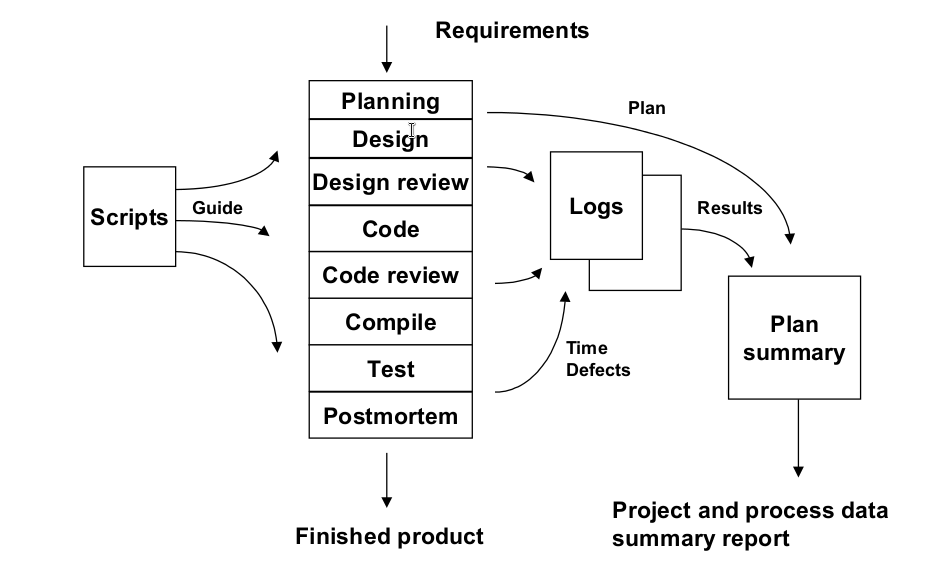
\includegraphics[ width=\textwidth , keepaspectratio]{./Images/PSPProcessStructure.png}\\[-1em]
\vspace{0.25cm}
\caption{PSP Process Flow Diagram}
\label{fig:2}
\end{figure}
\bigskip
\noindent

The structure of the PSP process is shown conceptually in the Figure. Starting with a requirements statement, the first step in the PSP process is planning. There is a planning script that guides this work and a plan summary for recording the planning data. While the engineers are following the script to do the work, they record their time and defect data on the time and defect logs. At the end of the job, during the postmortem phase (PM), they summarize the time and defect data from the logs, measure the program size, and enter these data in the plan summary form. When done, they deliver the finished product along with the completed plan
summary form.
\\

\begin{figure}[H]
\centering
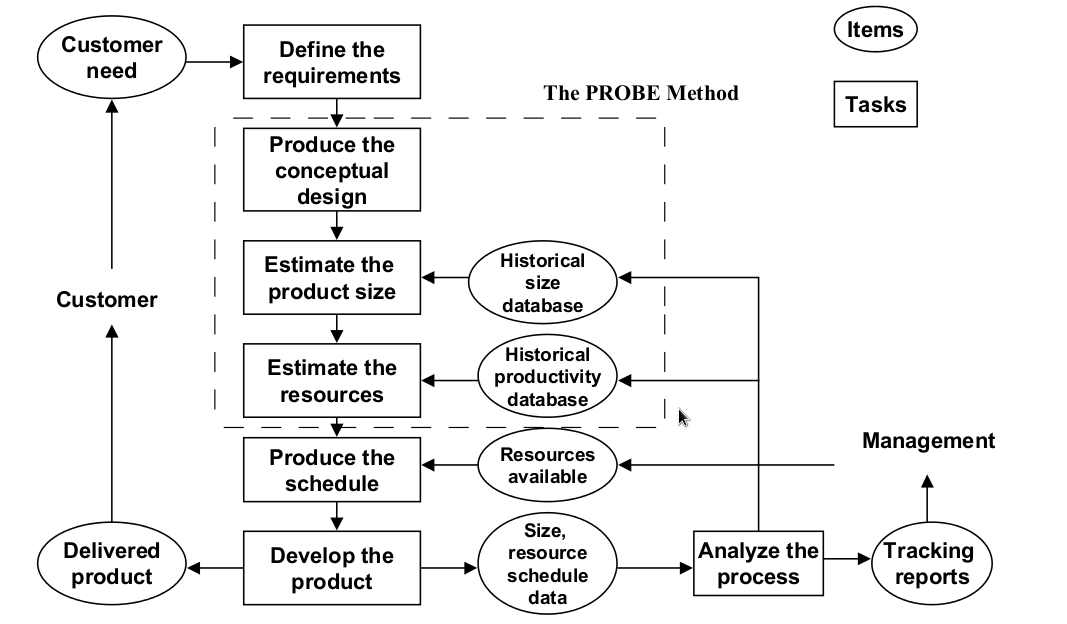
\includegraphics[ width=\textwidth , keepaspectratio]{./Images/PSPPlaningProcess.png}\\[-1em]
\vspace{0.25cm}
\caption{PSP Planning Process Diagram}
\label{fig:2}
\end{figure}
\bigskip

\noindent
\textbf{Requirements} \\
Engineers start planning by defining the work that needs to be done in as
much detail as possible. If all they have is a one-sentence requirements statement, then that
statement must be the basis for the plan
\\

\noindent
\textbf{Conceptual Design}. \\
To make an estimate and a plan, engineers first define how the product is to be designed and built. However, since the planning phase is too early to produce a complete product design, engineers produce what is called a conceptual design. This is a first, rough guess at what the product would look like if the engineers had to build it based on what they currently know. Later, during the design phase, the engineers examine design alternatives and produce a complete product design.
\\


\subsubsection{Notes on the Go Programming Language Design \textsuperscript{[4]}}
\noindent
The Go programming language was conceived in late 2007 as an answer to some of the problems that were being seen in developing software infrastructure at Google. Today`s programs may comprise of tens of millions of lines of code, are worked on by hundreds or even thousands of programmers, and are updated literally every day. To make matters worse, build times, even on large compilation clusters, have stretched to many minutes, even hours.
\\

Go was designed and developed to make working in this environment more productive. Besides its better-known aspects such as built-in concurrency and \gls{garbage collection}, Go's design considerations include rigorous dependency management, the adaptability of software architecture as systems grow, and robustness across the boundaries between components.
\\

Go is a compiled, concurrent, garbage-collected, \gls{statically typed} language developed at Google. It is an \gls{open source} project: Google imports the public repository rather than the other way around. Go is efficient, scalable, and productive.
\\

The goals of the Go project were to eliminate the slowness and clumsiness of software development at Google, and thereby to make the process more productive and scalable. The language was designed by and for people who write, read and debug and maintain large software systems.
\\
\noindent
The primary considerations in developing the Go programming language were:
\begin{easylist}
& \thinspace It must work at scale, for large programs with large numbers of dependencies, with large teams of programmers working on them.
& \thinspace It must be familiar, roughly C-like.The need to get programmers productive quickly in a new language means that the language cannot be too radical.
& \thinspace It must be modern. C, C++, and to some extent Java are quite old, designed before the advent of multi-core machines, networking, and web application development. There are features of the modern world that are better met by newer approaches, such as built-in concurrency.
\end{easylist}
\bigskip

\noindent
\textbf{Dependencies in Go} \\
Dependencies are defined, syntactically and semantically, by the language. They are explicit, clear, and ``computable``, which is to say, easy to write tools to analyze.
\begin{easylist}
& \thinspace language defines that unused dependencies are a compile-time error
& \thinspace Package invocations are transitive and restricted to the other packages imported by the package thus improving compilation time.
& \thinspace To make compilation even more efficient, the \gls{object file} is arranged so the export data is the first thing in the file, so the compiler can stop reading as soon as it reaches the end of that section.
& \thinspace Another feature of the Go dependency graph is that it has no cycles. The language defines that there can be no circular imports in the graph, and the \gls{compiler} and \gls{linker} both check that they do not exist.
\end{easylist}
\bigskip


\noindent
\textbf{Packages} 
\begin{easylist}
& \thinspace The design of Go's package system combines some of the properties of libraries, \gls{namespaces}, and modules into a single construct.
& \thinspace An important property of Go's package system is that the package path, being in general an arbitrary string, can be co-opted to refer to remote repositories by having it identify the \Gls{URL} of the site serving the repository.
\end{easylist}
\newpage

\noindent
\textbf{Syntax} 
\begin{easylist}
& \thinspace  Go was therefore designed with clarity and tooling in mind, and has a clean syntax.
& \thinspace Unlike C and Java and especially C++, Go can be parsed without \gls{type information} or a \gls{symbol table}; there is no type-specific context. The grammar is easy to reason about and therefore tools are easy to write.
& \thinspace Function syntax is straightforward for simple functions. A method is just a function with a special parameter, its receiver, which can be passed to the function using the standard "dot" notation. Go has \gls{first-class functions} and \gls{closures}. Finally, in Go functions can return multiple values.
& \thinspace One feature missing from Go is that it does not support default function arguments. One mitigating factor for the lack of default arguments is that Go has easy-to-use, \gls{type-safe} support for \gls{variadic functions}.
\end{easylist}
\bigskip

\noindent
\textbf{Naming} 
\begin{easylist}
& \thinspace Go takes an unusual approach to defining the visibility of an \gls{identifier}. The case of the initial letter of the identifier determines the visibility. If the initial character is an upper case letter, the identifier is exported (public); otherwise it is not.
& \thinspace Another simplification is that Go has a very compact scope hierarchy: 
&& universe (predeclared identifiers such as int and string)
&& package (all the source files of a package live at the same scope)
&& file (for package import renames only; not very important in practice)
&& function 
&& block 
& \thinspace The rules for naming provide an important property for scaling because they guarantee that adding an exported name to a package can never break a client of that package. The naming rules decouple packages, providing scaling, clarity, and robustness.
\end{easylist}
\bigskip

\noindent
\textbf{Semantics} 
\begin{easylist}
& \thinspace The semantics of Go statements is generally C-like. That said, Go makes many small changes to C semantics, mostly in the service of robustness. These include:
&& there is no pointer arithmetic
&& there are no implicit numeric conversions
&& array bounds are always checked
&& there are no type aliases (after type X int, X and int are distinct types not aliases)
&& ++ and -- are statements not expressions
&& assignment is not an expression
&& it is legal (encouraged even) to take the address of a stack variable
& \thinspace There are some much bigger changes too, stepping far from the traditional C, C++, and even Java models. These include linguistic support for:
&& concurrency
&& garbage collection
&& interface types
&& \gls{reflection}
&& type switches
\end{easylist}
\bigskip

\noindent
\textbf{\Gls{Concurrency}} \\
Concurrency is important to the modern computing environment with its multi-core machines running web servers with multiple clients, what might be called the typical Google program. This kind of software is not especially well served by C++ or Java, which lack sufficient concurrency support at the language level.
\bigskip

\noindent
\textbf{Garbage Collection} \\
Go has no explicit memory-freeing operation: the only way allocated memory returns to the pool is through the garbage collector. The language is much easier to use because of garbage collection. 
\bigskip

\noindent
\textbf{\Gls{Composition} not \Gls{inheritance}} \\
Go takes an unusual approach to object-oriented programming, allowing methods on any type, not just classes, but without any form of type-based inheritance like sub-classing. This means there is no type hierarchy.
Instead, Go has interfaces.  In Go an interface is just a set of methods. A type will usually satisfy many interfaces, each corresponding to a subset of its methods. Go encourages composition over inheritance, using simple, often one-method interfaces to define trivial behaviors that serve as clean, comprehensible boundaries between components.
\bigskip

\noindent
\textbf{Error} \\
Go does not have an exception facility in the conventional sense, that is, there is no control structure associated with \gls{error handling}. The key language feature for error handling is a pre-defined interface type called error that represents a value that has an Error method returning a string.

\subsection{Data Models \& Diagrams}

\begin{sideways}
\centering
	\begin{minipage}{\textheight}
	\centering
	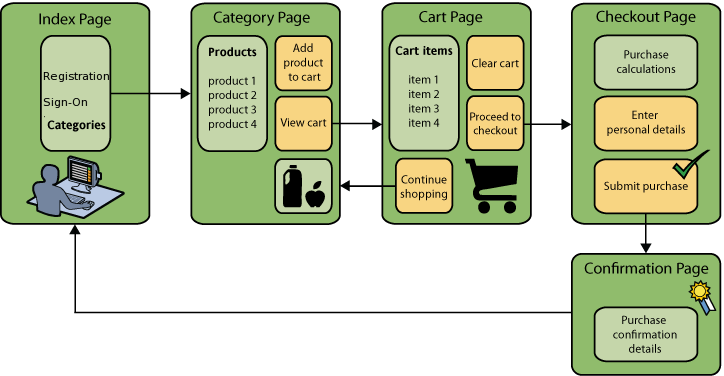
\includegraphics[ width=0.86\textheight , keepaspectratio ]{./Images/processflow1.png}\\[-1em]
	%\vspace{0.25cm}
	\captionof{figure}{Process Flow Diagram}
	\label{fig:3}
	\end{minipage}
\end{sideways}

\begin{figure}[H]
\centering
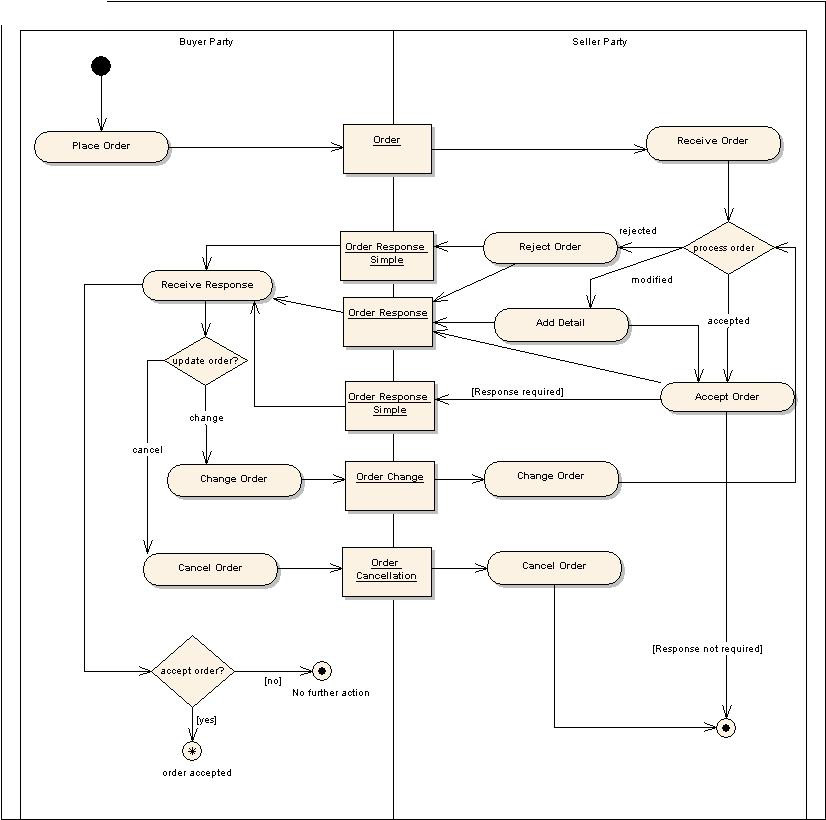
\includegraphics[ width=\textwidth , keepaspectratio]{./Images/OrderingProcess.jpg}\\[-1em]
\vspace{0.25cm}
\caption{Ordering Process Flow Diagram}
\label{fig:4}
\end{figure}

\begin{sideways}
\centering
	\begin{minipage}{\textheight}
	\centering
	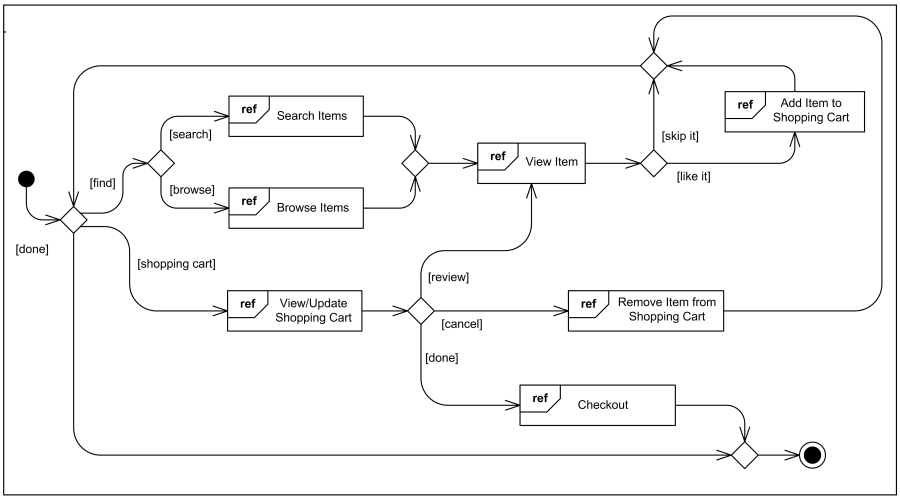
\includegraphics[ width=0.86\textheight , keepaspectratio]{./Images/processflow2.png}\\[-1em]
	\vspace{0.25cm}
	\captionof{figure}{Shopping Cart Process Flow Diagram}
	\label{fig:5}
	\end{minipage}
\end{sideways}


\begin{sideways}
\centering
	\begin{minipage}{\textheight}
	\centering
	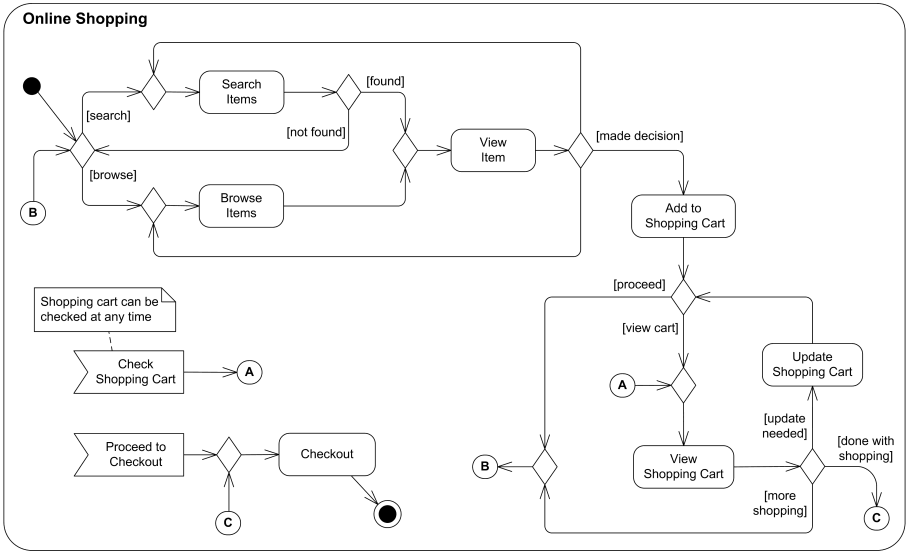
\includegraphics[ width=0.86\textheight , keepaspectratio]{./Images/activity-examples-online-shopping.png}\\[-1em]
	%\vspace{0.25cm}
	\captionof{figure}{Shopping Cart Activity Flow Diagram}
	\label{fig:6}
	\end{minipage}
\end{sideways}


\begin{sideways}
\centering
	\begin{minipage}{\textheight}
	\centering
	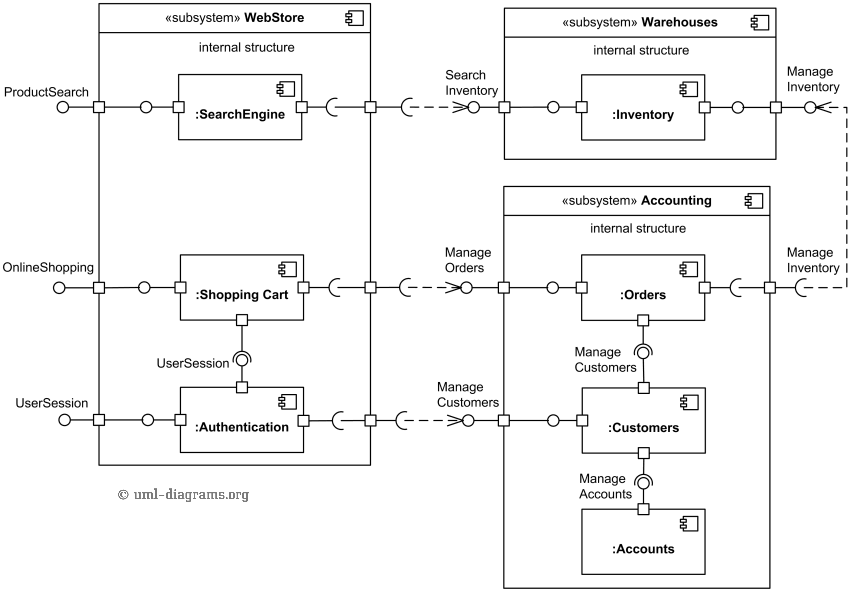
\includegraphics[ width=0.76\textheight , keepaspectratio]{./Images/componentwebsite.png}\\[-1em]
	%\vspace{0.25cm}
	\captionof{figure}{Website Component Diagram}
	\label{fig:7}
	\end{minipage}
\end{sideways}


\begin{minipage}{\textwidth}
	\centering
	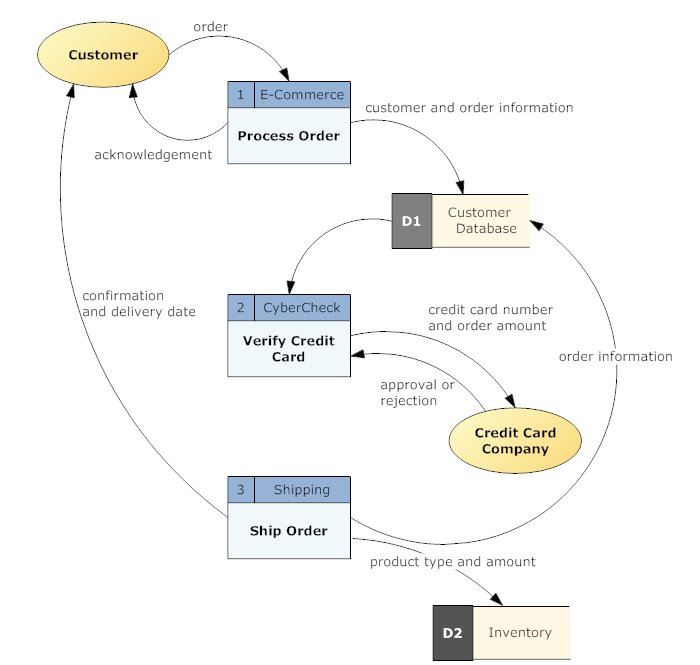
\includegraphics[ width=\textwidth , keepaspectratio]{./Images/dfd1.png}\\[-1em]
	%\vspace{0.25cm}
	\captionof{figure}{Data Flow Diagram}
	\label{fig:8}
\end{minipage}

\vspace{3cm}

\begin{minipage}{\textwidth}
	\centering
	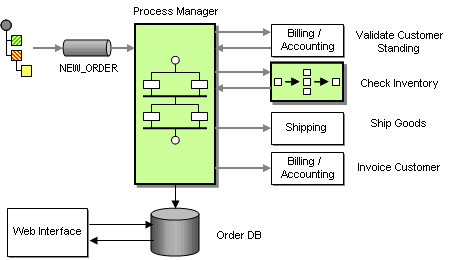
\includegraphics[ width=\textwidth , keepaspectratio]{./Images/architecture.png}\\[-1em]
	\vspace{0.25cm}
	\captionof{figure}{Architecture Diagram}
	\label{fig:9}
\end{minipage}


\newpage
%*******************************************SECTION**********************************
\section{\MakeUppercase{System Design}}

\subsection{Modularization Details}

\begin{center}
	{
	\setlength{\extrarowheight}{2pt}

	\newcolumntype{b}{X}
	\newcolumntype{s}{>{\hsize=.4\hsize}X}
	\newcolumntype{t}{>{\hsize=1.3\hsize}X}
		
	%\renewcommand\thetable{2} 					
	%\captionof{table}{ \textbf {\small {Modularization Details}}} \label{table:2}
	\vspace{0.25cm}
									
	\begin{tabularx}{\textwidth}{ | >{\ttfamily\raggedright\arraybackslash} s 
	| >{\ttfamily\raggedright\arraybackslash} t 
	| >{\ttfamily\raggedright\arraybackslash} t | }
	
	\caption{ \textbf {\small {Modularization Details}}} \\
								
	\hline
								
	{\textbf{\textcolor{black}{{Sr. No.} \newline}}} & {\textbf{\textcolor{black}{ {Module}}}} & \textbf{\textcolor{black}{ {Description}}} \\
								
	\hline
	1.0 & User Registration \& Sign-On & Users can register on the website. Users need to authenticate during login  \\
	\hline	
	2.0 & Manage Session & Unique session is created for every user after login. Session is destroyed after user logs out \\
	\hline			
	3.0 & Shopping Cart & Javascript module for users to add items to shopping cart   \\
	\hline
	4.0 & Product Search & Javsacript function for users to be able to search for products using the name string  \\ [1em]
	\hline
	5.0 & Place Order & Triggers order for the selected items in the Cart. A unique Order ID is generated and details are saved to the Database  \\  [1em]
	\hline	  
	6.0 & Stripe \Gls{Payment Gateway} & \Gls{API} to receive payments for Orders \\ 
	\hline	
	7.0 & Email Notification for Order Confirmation & Automated \gls{email} notification on successful order and successful payment for the order \\ [1em]
	\hline	
	8.0 & Manage Products & Utility to add products to the database that includes the File Upload Handler \\ [1em]
	\hline	 
	9.0 & File Upload Handler & Utility to add Product image when uploading details of a new product  \\ [1em]
	\hline	  
	10.0 & View Orders & Admin user can query and view details of Placed orders  \\ [1em]
	\hline
	11.0 & View Specific Order & Admin user can query and view details of a specific order  \\ [1em]	
	\hline
	\end{tabularx}
	}
\end{center}
						
\bigskip
\noindent

%\subsection{Data integrity \& Constraints}
\newpage
\subsection{Database Design}

Database design is the process of producing a detailed data model of database. This data model contains all the needed logical and physical design choices and physical storage parameters needed to generate a design in a data definition language, which can then be used to create a database.
\bigskip


\begin{minipage}{\textwidth}
	\centering
	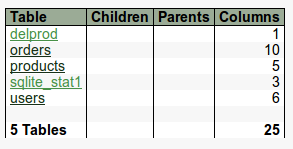
\includegraphics[ width=0.7\textwidth , keepaspectratio]{./Images/SS7.png}\\[-1em]
	\vspace{0.25cm}
	\captionof{figure}{List of Database Tables}
	\label{fig:9}
\end{minipage}

\vspace{3cm}

\begin{minipage}{\textwidth}
	\centering
	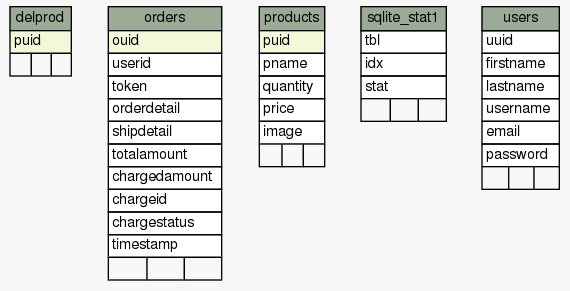
\includegraphics[ width=\textwidth , keepaspectratio]{./Images/SS8.png}\\[-1em]
	\vspace{0.25cm}
	\captionof{figure}{Utility Tables with data Elements}
	\label{fig:9}
\end{minipage}

%\vspace{3cm}

\begin{minipage}{\textwidth}
	\centering
	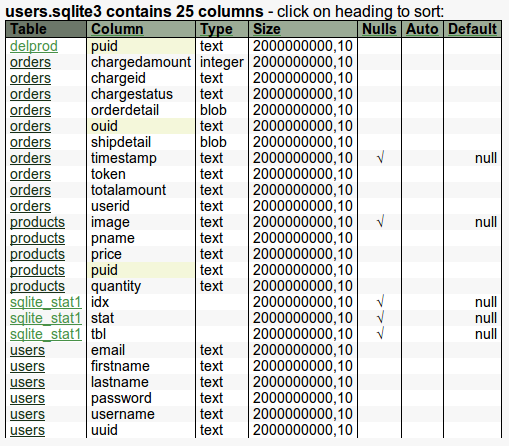
\includegraphics[ width=\textwidth , keepaspectratio]{./Images/SS9.png}\\[-1em]
	\vspace{0.25cm}
	\captionof{figure}{Data Elements type and size}
	\label{fig:9}
\end{minipage}

\vspace{3cm}

\begin{minipage}{\textwidth}
	\centering
	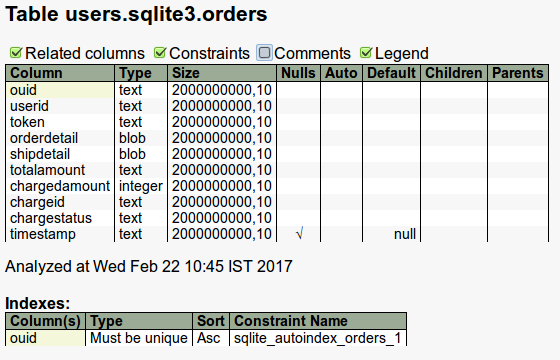
\includegraphics[ width=\textwidth , keepaspectratio]{./Images/SS4.png}\\[-1em]
	\vspace{0.25cm}
	\captionof{figure}{Order table}
	\label{fig:9}
\end{minipage}

%\vspace{3cm}

\begin{minipage}{\textwidth}
	\centering
	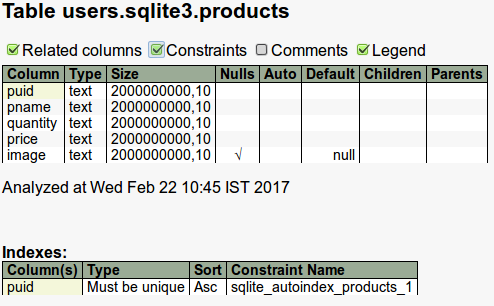
\includegraphics[ width=\textwidth , keepaspectratio]{./Images/SS5.png}\\[-1em]
	\vspace{0.25cm}
	\captionof{figure}{Product table}
	\label{fig:9}
\end{minipage}

\vspace{2cm}

\begin{minipage}{\textwidth}
	\centering
	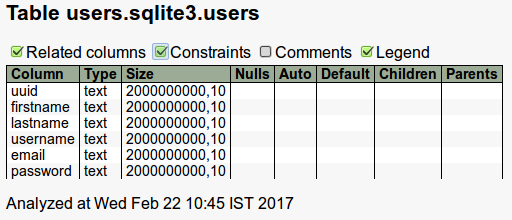
\includegraphics[ width=\textwidth , keepaspectratio]{./Images/SS6.png}\\[-1em]
	\vspace{0.25cm}
	\captionof{figure}{User table}
	\label{fig:9}
\end{minipage}

\vspace{2cm}

\begin{minipage}{\textwidth}
	\centering
	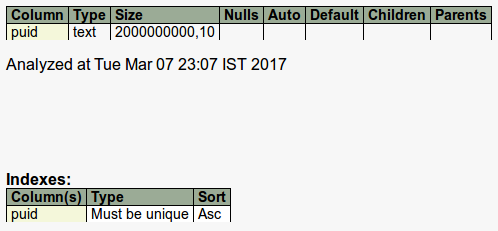
\includegraphics[ width=\textwidth , keepaspectratio]{./Images/SS10.png}\\[-1em]
	\vspace{0.25cm}
	\captionof{figure}{Delete Product table}
	\label{fig:9}
\end{minipage}
\bigskip

\noindent
JSON (JavaScript Object Notation) is a lightweight data-interchange format. It is easy for humans to read and write. It is easy for machines to parse and generate. \\
JSON is a format that encodes objects in a string. Serialization means to convert an object into that string, and deserialization is its inverse operation. When transmitting data or storing them in a file, the data are required to be byte strings.\\

\noindent
The `orderdetails` and `shipdetails`fields are maintained as JSON data (Blob type) in the `Orders` table of the database  

\begin{minipage}{\textwidth}
	\centering
	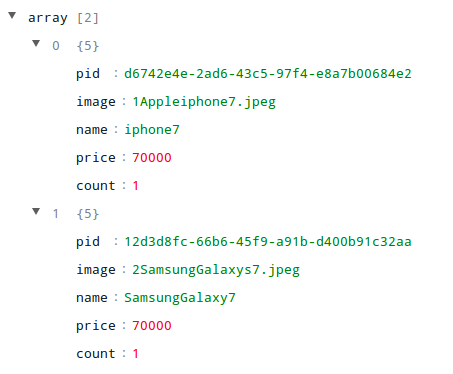
\includegraphics[ width=\textwidth , keepaspectratio]{./Images/JSONOrderDetailsField.png}\\[-1em]
	\vspace{0.25cm}
	\captionof{figure}{Orderdetails Field JSON Structure}
	\label{fig:9}
\end{minipage}

\vspace{2cm}

\begin{minipage}{\textwidth}
	\centering
	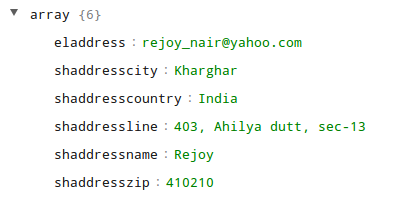
\includegraphics[ width=\textwidth , keepaspectratio]{./Images/JSONShipdetail.png}\\[-1em]
	\vspace{0.25cm}
	\captionof{figure}{Shipdetails Field JSON Structure}
	\label{fig:9}
\end{minipage}
\bigskip

\begin{minipage}{\textwidth}
	\centering
	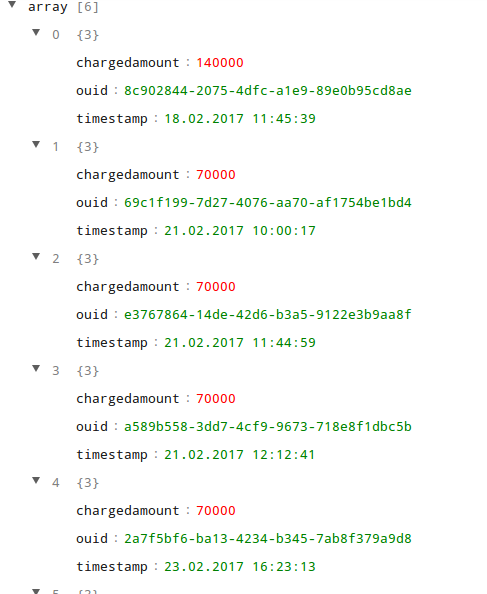
\includegraphics[ width=\textwidth , keepaspectratio]{./Images/JsonarrayViewOrder.png}\\[-1em]
	\vspace{0.25cm}
	\captionof{figure}{JSON Array View Order}
	\label{fig:9}
\end{minipage}
\bigskip

\begin{sideways}
\centering
	\begin{minipage}{\textheight}
	\centering
	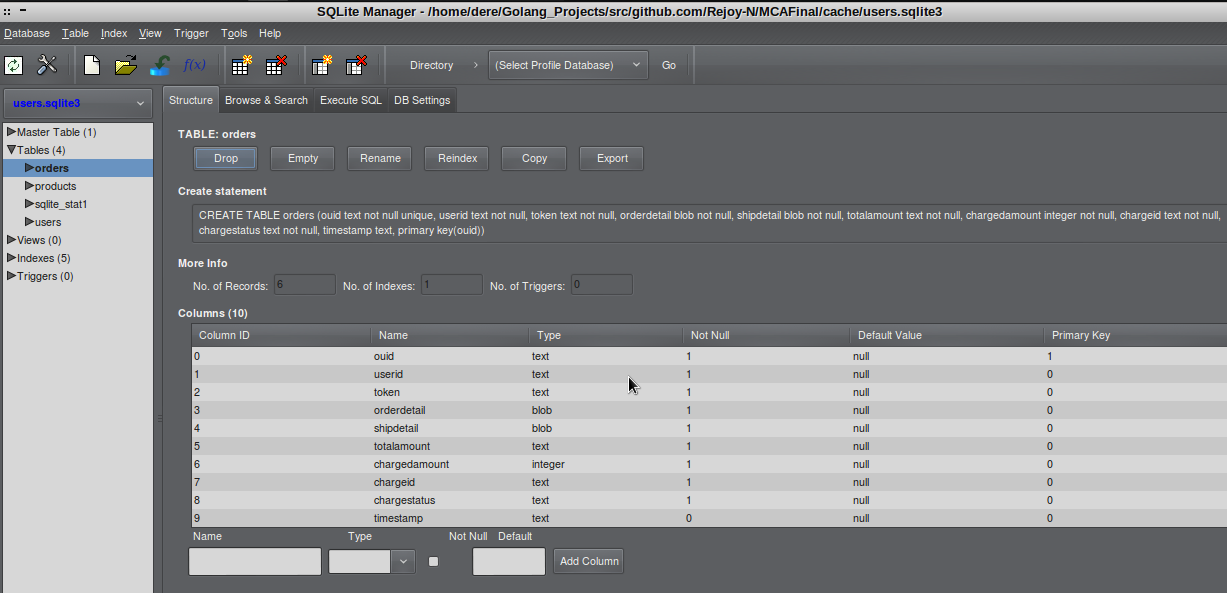
\includegraphics[ width=\textheight , keepaspectratio]{./Images/DBOrder1.png}\\[-1em]
	%\vspace{0.25cm}
	\captionof{figure}{Order table viewed in SQLite Manager }
	\label{fig:7}
	\end{minipage}
\end{sideways}

\noindent
With local storage, web applications can store data locally within the user`s browser.Local storage is more secure, and large amounts of data can be stored locally, without affecting website performance.\\
\bigskip

\begin{minipage}{\textwidth}
	\centering
	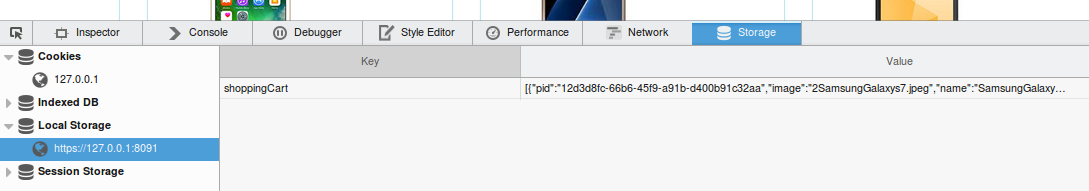
\includegraphics[ width=\textwidth , keepaspectratio]{./Images/LocalStorage.png}\\[-1em]
	\vspace{0.25cm}
	\captionof{figure}{HTML Local Storage}
	\label{fig:9}
\end{minipage}
\bigskip

\noindent
An HTTP cookie (also called web cookie, Internet cookie, browser cookie or simply cookie) is a small piece of data sent from a website and stored on the user`s computer by the user`s web browser while the user is browsing. Cookies were designed to be a reliable mechanism for websites to remember stateful information (as in this case items added in the shopping cart in an online store) \\
\bigskip

\begin{minipage}{\textwidth}
	\centering
	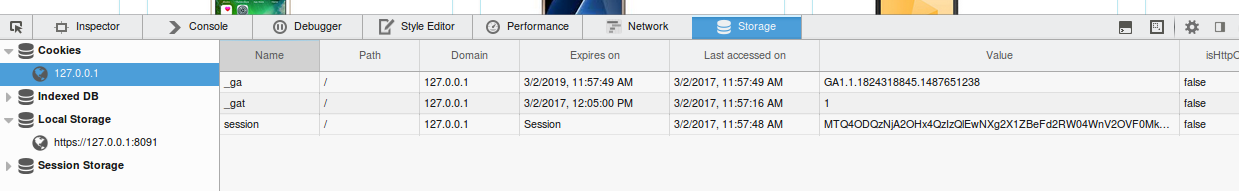
\includegraphics[ width=\textwidth , keepaspectratio]{./Images/SessionCookies.png}\\[-1em]
	\vspace{0.25cm}
	\captionof{figure}{Browser Session Cookies}
	\label{fig:9}
\end{minipage}
\bigskip

\subsection{User Interface Design}

User interface design (UI) or user interface engineering is the design of user interfaces for machines and software, such as computers, home appliances, mobile devices, and other electronic devices, with the focus on maximizing usability and the user experience. The goal of user interface design is to make the user`s interaction as simple and efficient as possible, in terms of accomplishing user goals (user-centered design).\textsuperscript{ 5}

A good e-commerce site should present the following factors to users for better usability
\begin{easylist}
& \thinspace Simple navigation from home page to information and order links for specific products
& \thinspace Obvious shopping links or buttons
& \thinspace Effective categorical Organization of products
& \thinspace Easy scanning and selecting items on list
& \thinspace Consistent layout of product information
& \thinspace Minimal or effective security notification or messages
& \thinspace Knowing when an item was saved or not saved in the shopping cart
\end{easylist}
\bigskip
\noindent

\begin{sideways}
    \centering
		\begin{minipage}{\textheight}
		\centering
		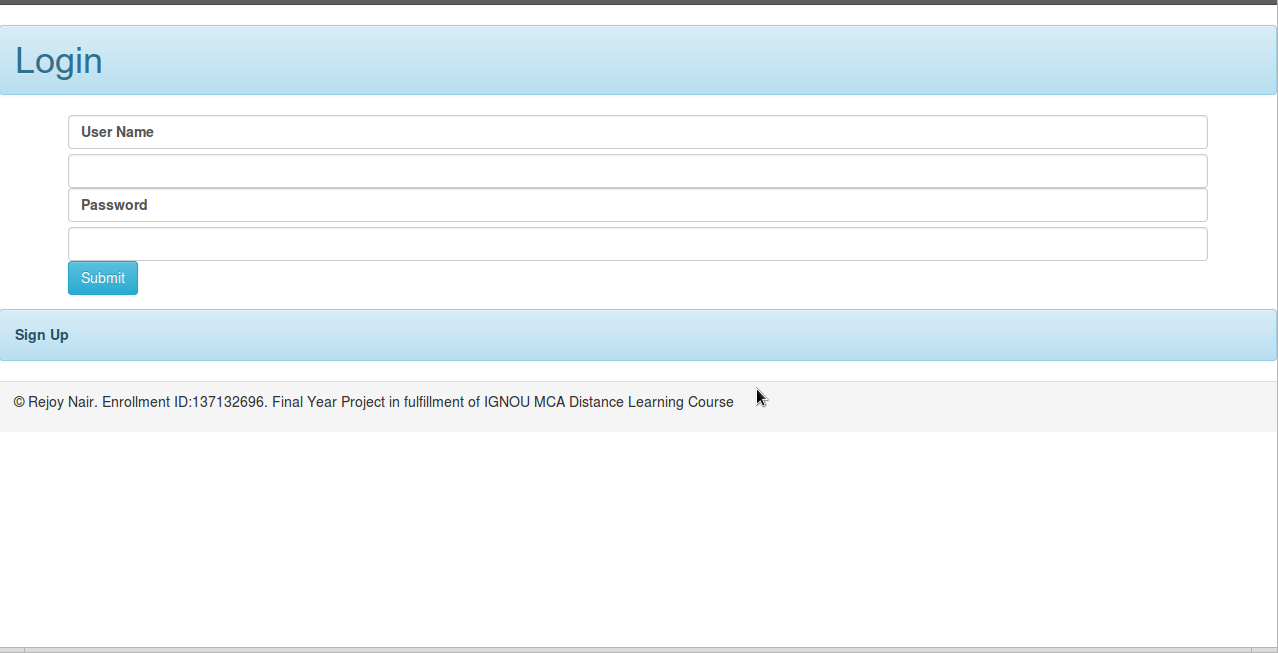
\includegraphics[ width=\textheight , keepaspectratio ]{./Images/MainScreen.png}\\[-1em]
		\captionof{figure}{Customer Login Screen}
		%\vspace{0.25cm}
		\label{fig:2}
		\end{minipage}		
\end{sideways}

\begin{center}
	{
	\setlength{\extrarowheight}{2pt}

	\newcolumntype{b}{X}
	\newcolumntype{s}{>{\hsize=.4\hsize}X}
	\newcolumntype{t}{>{\hsize=1.3\hsize}X}
		
	%\renewcommand\thetable{2} 					
	%\captionof{table}{ \textbf {\small {Customer Login Screen}}} \label{table:2}
	\vspace{0.25cm}
									
	\begin{tabularx}{\textwidth}{ | >{\ttfamily\raggedright\arraybackslash} s 
	| >{\ttfamily\raggedright\arraybackslash} t 
	| >{\ttfamily\raggedright\arraybackslash} t | }
	
	\caption{ \textbf {\small {User Login}}} \\
								
	\hline
								
	{\textbf{\textcolor{black}{{Sr. No.} \newline}}} & {\textbf{\textcolor{black}{{Input Element}}}} & \textbf{\textcolor{black}{{Description \& Behaviour}}} \\
								
	\hline
	1.0 & Username Input Field & Textbox to accept registered username. Email ID or any other unique attribute shall not be accepted \\
	\hline		
	2.0 & Password Input Field & Textbox to accept password associated with the Username  \\
	\hline	  	 
	3.0 & Submit Button & To post the Username and password entered by the user to the server  \\
	\hline	
	4.0 & Alert & To notify User of incorrect or empty Username and / or password or an expired User session  \\
	\hline		   		       	           								
	\end{tabularx}
	}
\end{center}

\begin{sideways}
    \centering
		\begin{minipage}{\textheight}
		\centering
		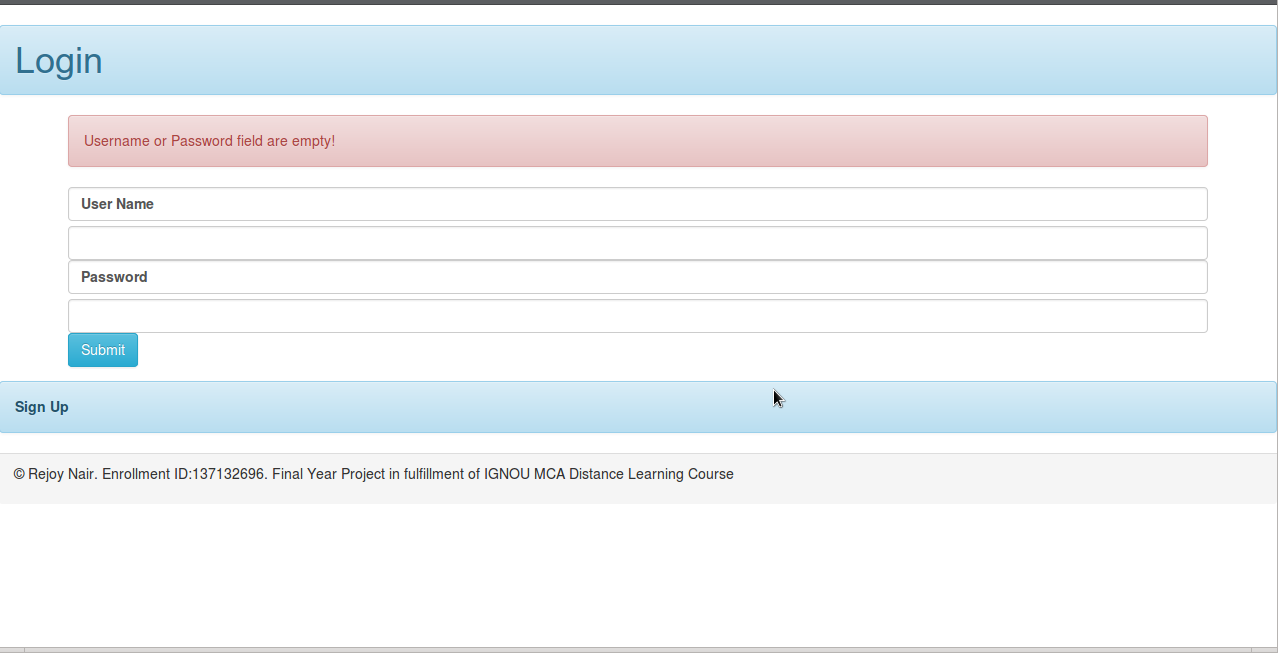
\includegraphics[ width=\textheight , keepaspectratio ]{./Images/LoginValidation.png}\\[-1em]
		%\vspace{0.25cm}
		\captionof{figure}{Customer Login Screen - Alert}
		\label{fig:2}
		\end{minipage}
\end{sideways}


\begin{sideways}
    \centering
		\begin{minipage}{\textheight}
		\centering
		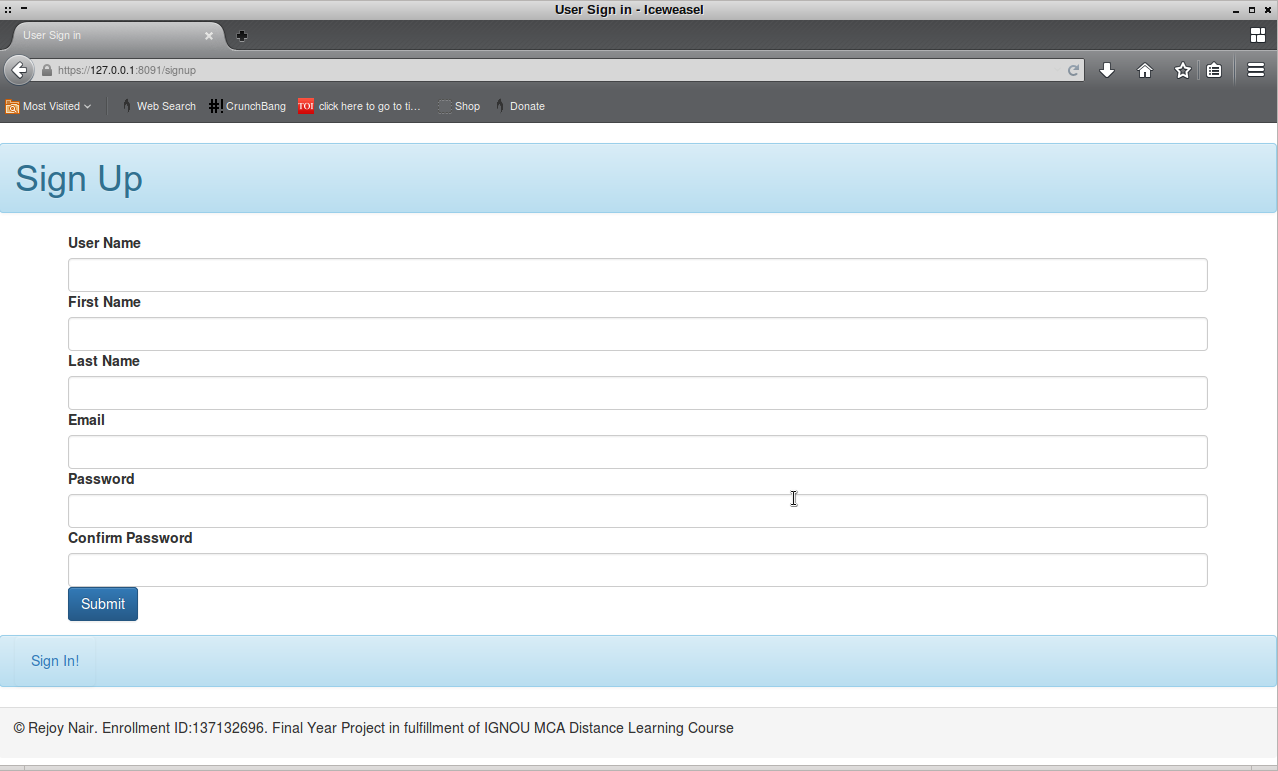
\includegraphics[width=0.86\textheight , keepaspectratio ]{./Images/SignupScreen.png}\\[-1em]
		%\vspace{0.25cm}
		\captionof{figure}{Customer Sign-up Screen}
		\label{fig:2}
		\end{minipage}
\end{sideways}


\begin{center}
	{
	\setlength{\extrarowheight}{2pt}

	\newcolumntype{b}{X}
	\newcolumntype{s}{>{\hsize=.4\hsize}X}
	\newcolumntype{t}{>{\hsize=1.3\hsize}X}
		
	%\renewcommand\thetable{2} 					
	%\captionof{table}{ \textbf {\small {Customer Signup Screen}}} \label{table:2}
	\vspace{0.25cm}
									
	\begin{tabularx}{\textwidth}{ | >{\ttfamily\raggedright\arraybackslash} s 
	| >{\ttfamily\raggedright\arraybackslash} t 
	| >{\ttfamily\raggedright\arraybackslash} t | }
	
	\caption{ \textbf {\small {Customer Signup Screen}}} \\
								
	\hline
								
	{\textbf{\textcolor{black}{{Sr. No.} \newline}}} & {\textbf{\textcolor{black}{{Input Element}}}} & \textbf{\textcolor{black}{{Description \& Behaviour}}} \\
								
	\hline
	1.0 & Username Input Field & Textbox to accept username that the user wishes to register with. Username will have to be unique \\
	\hline		
	2.0 & First Name Input Field & Textbox to accept first name that the user wishes to register with.  \\
	\hline	  	 
	3.0 & Last Name Input Field & Textbox to accept last name that the user wishes to register with. \\
	\hline	  	 	
	4.0 & Email Input Field & Textbox to accept \gls{email} address that the user wishes to register with.  \\
	\hline	  	 
	5.0 & Password Input Field & Textbox to create a password for the username that the user wishes to register with.  \\
	\hline	  
	6.0 & Confirm Password Input Field & Textbox to reconfirm the entered password at the time of registration \\
	\hline			 		
	7.0 & Submit Button & To post the details contained in the sign-up form as entered by the user to the server  \\
	\hline	
	8.0 & Alert & To notify User of incorrect or empty or invalid input entries for each of the fields of the sign-up form  \\
	\hline		   		       	           								
	\end{tabularx}
	}
\end{center}
						

\begin{sideways}
    \centering
		\begin{minipage}{\textheight}
		\centering
		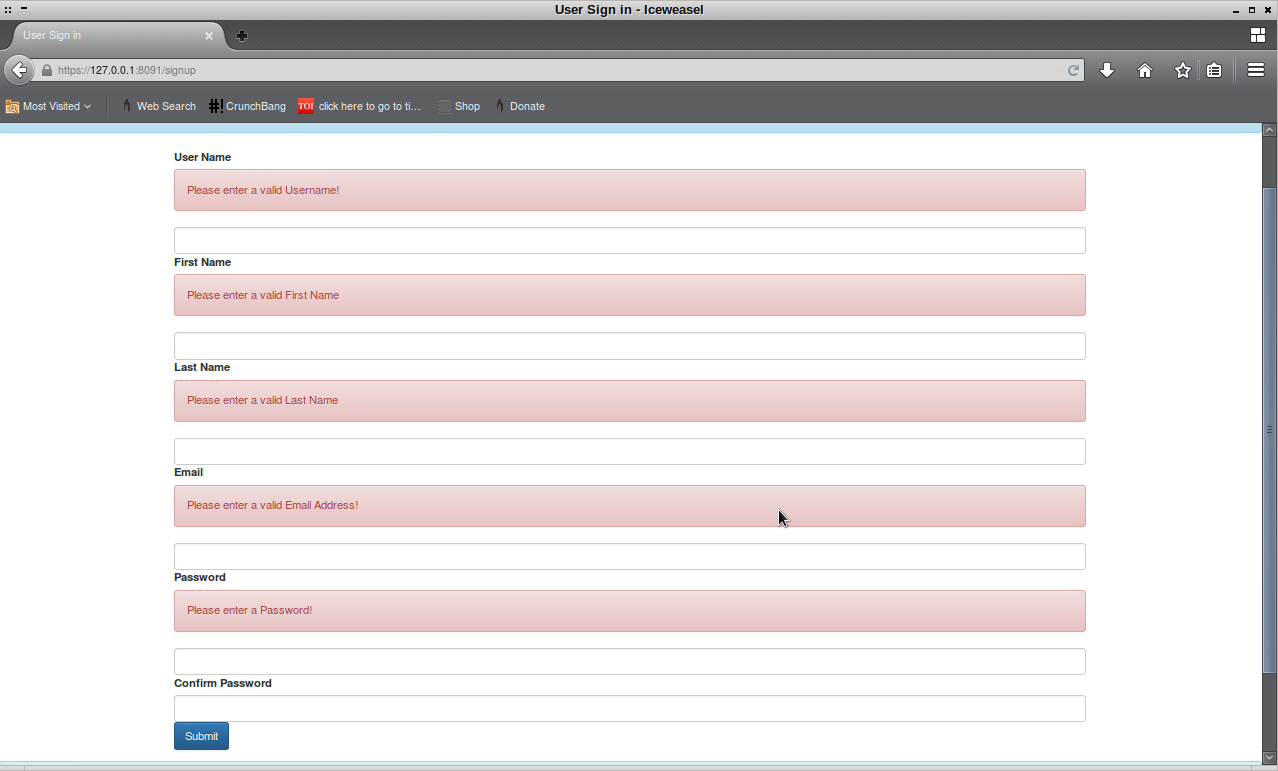
\includegraphics[ width=0.86\textheight , keepaspectratio ]{./Images/SignupScreenVallidation.png}\\[-1em]
		%\vspace{0.25cm}
		\captionof{figure}{Customer Sign-up Screen Validations}
		\label{fig:2}
		\end{minipage}
\end{sideways}


\begin{sideways}
    \centering
		\begin{minipage}{\textheight}
		\centering
		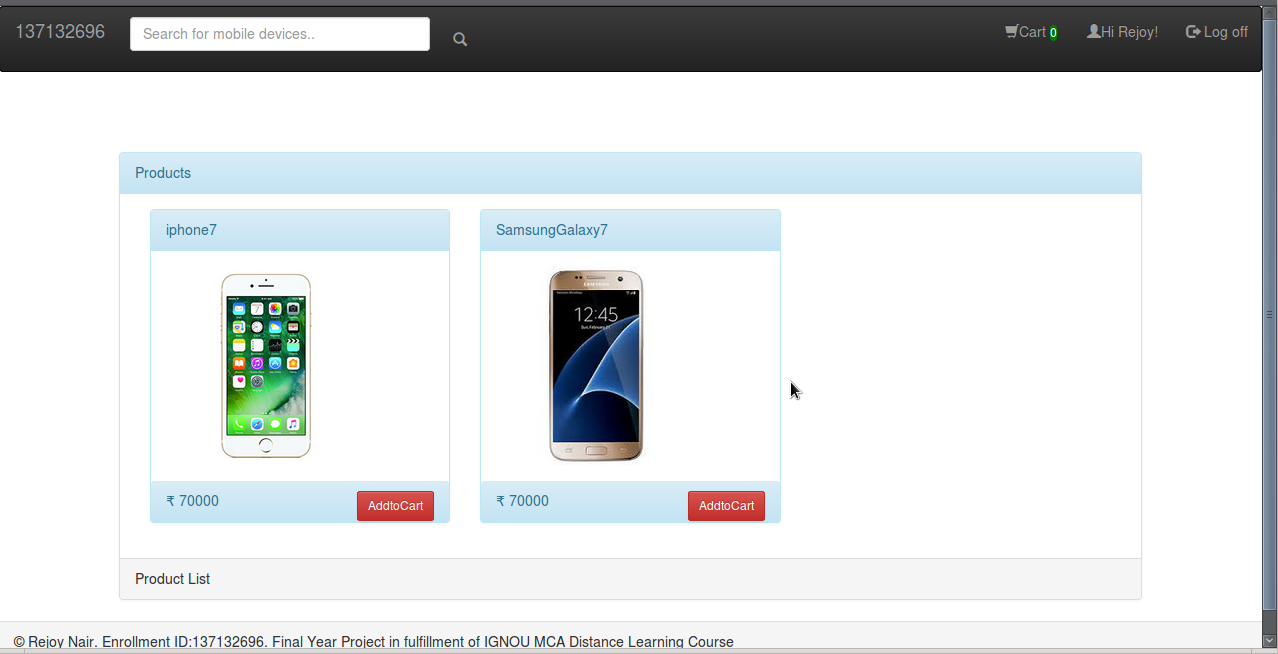
\includegraphics[ width=\textheight , keepaspectratio ]{./Images/InternalScreen1.png}\\[-1em]
		%\vspace{0.25cm}
		\captionof{figure}{Customer Login Main View}
		\label{fig:2}
		\end{minipage}
\end{sideways}


\begin{center}
	{
	\setlength{\extrarowheight}{2pt}

	\newcolumntype{b}{X}
	\newcolumntype{s}{>{\hsize=.4\hsize}X}
	\newcolumntype{t}{>{\hsize=1.3\hsize}X}
		
	%\renewcommand\thetable{2} 					
	%\captionof{table}{ \textbf {\small {Customer Login Main View}}} \label{table:2}
	\vspace{0.25cm}
									
	\begin{tabularx}{\textwidth}{ | >{\ttfamily\raggedright\arraybackslash} s 
	| >{\ttfamily\raggedright\arraybackslash} t 
	| >{\ttfamily\raggedright\arraybackslash} t | }
	
	\caption{ \textbf {\small {Customer Login Main View}}} \\
								
	\hline
								
	{\textbf{\textcolor{black}{{Sr. No.} \newline}}} & {\textbf{\textcolor{black}{{Input Element}}}} & \textbf{\textcolor{black}{{Description \& Behaviour}}} \\
								
	\hline
	1.0 & Product Info Panel & Panel that contains description of the product such as name and price along with its image \\
	\hline		
	2.0 & Product Info Panel - Add to Cart Button & ``Add to Cart'' button on the product info panel that allows customers to add products to the cart \\
	\hline	  	 
	3.0 & Banner & Banner to place the brand logo. Currently contains the enrollment ID 137132696 \\
	\hline	  	 	
	4.0 & Search Box & Search box to filter products based on Product description  \\
	\hline	  	 
	5.0 & Shopping Cart & Icon which shows the count of the products added to the shopping cart. Clicking on the shopping cart displays the dropdown that contains the list of the products added to the cart along with the image, price, quantity and total amount per item  \\
	\hline	  
	6.0 & Shopping Cart- Quantity & Number input type that can be increased or decreased. Min Value is 1 \\
	\hline			 		
	7.0 & Shopping Cart- Button & ``-'' button to remove a single unit of the item from the total quantity. ``+'' to add a single unit to the existing quantity. ``X'' to completely remove the item from the shopping cart list  \\
	\hline	
	8.0 & Alert & To notify User of a product being added to the shopping cart  \\
	\hline	
	9.0 & User Profile & Link to the user Profile Page. By defaults shows the user first name.  \\
	\hline			
	10.0 & Logout & Allows the user to logout from the web portal  \\
	\hline		   		       	           								
	\end{tabularx}
	}
\end{center}


\begin{sideways}
    \centering
		\begin{minipage}{\textheight}
		\centering
		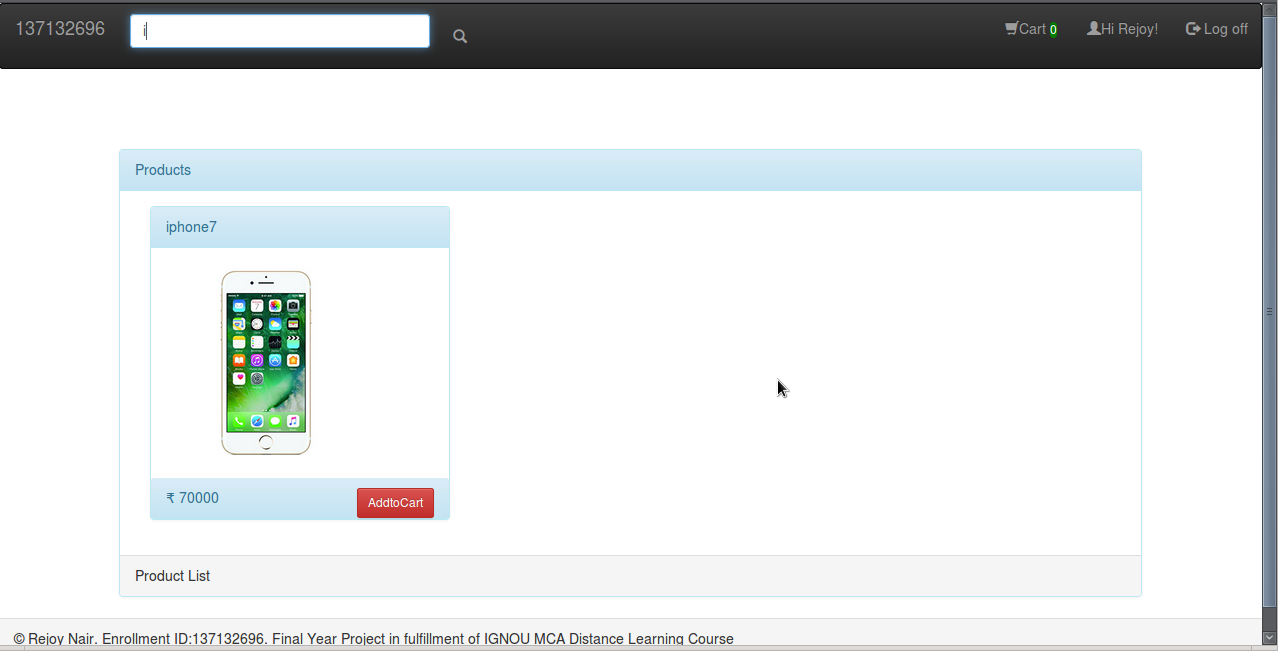
\includegraphics[ width=\textheight , keepaspectratio ]{./Images/InternalScreen2.png}\\[-1em]
		%\vspace{0.25cm}
		\captionof{figure}{Customer Login Main View - Search}
		\label{fig:2}
		\end{minipage}
\end{sideways}


\begin{sideways}
    \centering
		\begin{minipage}{\textheight}
		\centering
		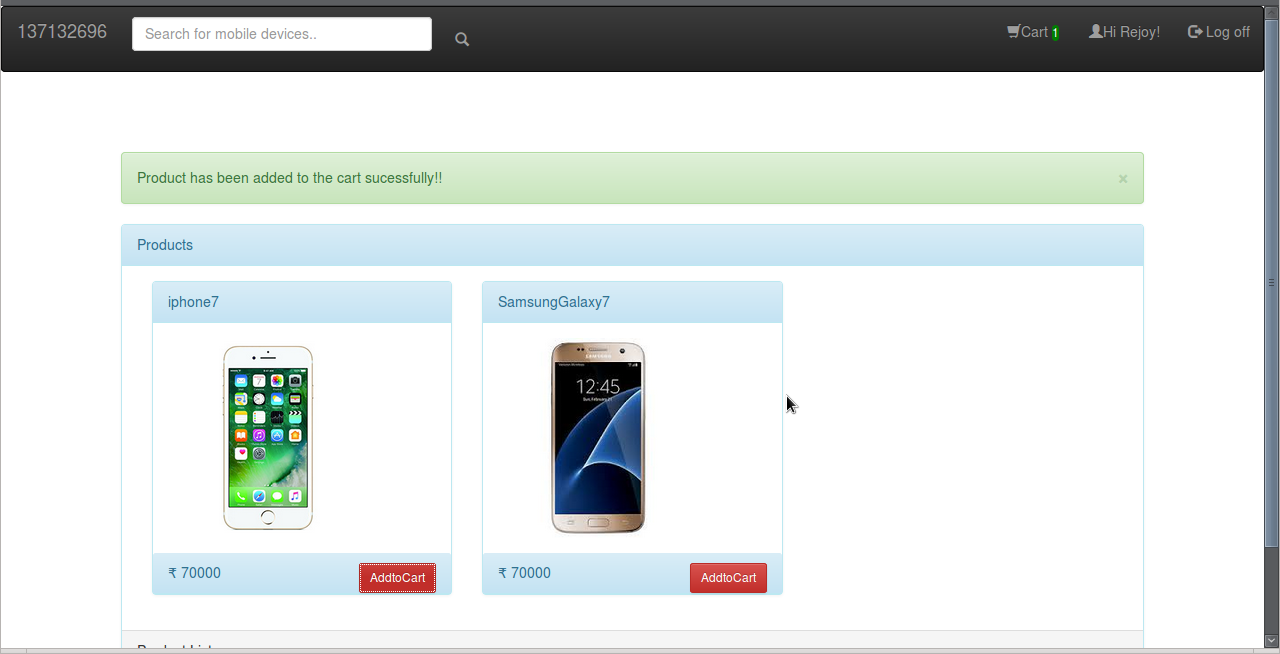
\includegraphics[ width=\textheight , keepaspectratio ]{./Images/internalScreen3.png}\\[-1em]
		%\vspace{0.25cm}
		\captionof{figure}{Customer Login Main View - Alert}
		\label{fig:2}
		\end{minipage}
\end{sideways}


\begin{sideways}
    \centering
		\begin{minipage}{\textheight}
		\centering
		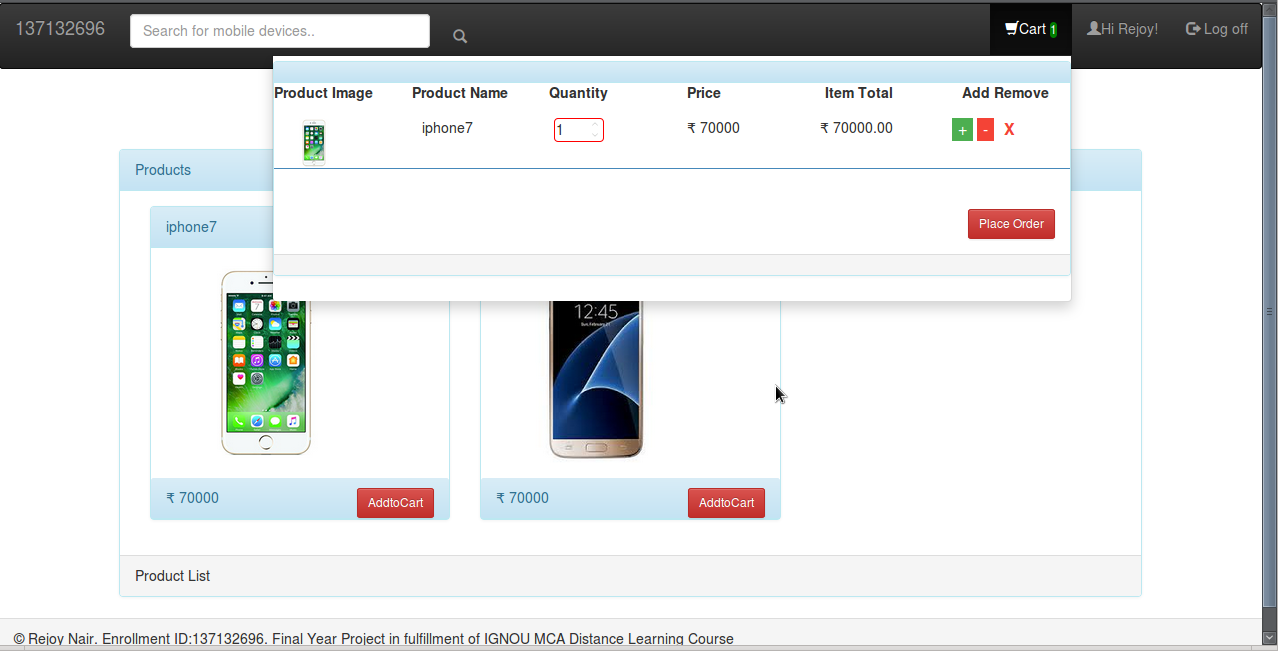
\includegraphics[ width=\textheight , keepaspectratio ]{./Images/InternalScreen4.png}\\[-1em]
		%\vspace{0.25cm}
		\captionof{figure}{Customer Login Main View - Shopping Cart}
		\label{fig:2}
		\end{minipage}
\end{sideways}


\begin{center}
	{
	\setlength{\extrarowheight}{2pt}

	\newcolumntype{b}{X}
	\newcolumntype{s}{>{\hsize=.4\hsize}X}
	\newcolumntype{t}{>{\hsize=1.3\hsize}X}
		
	%\renewcommand\thetable{2} 					
	%\captionof{table}{ \textbf {\small {Customer Login Main View}}} \label{table:2}
	\vspace{0.25cm}
									
	\begin{tabularx}{\textwidth}{ | >{\ttfamily\raggedright\arraybackslash} s 
	| >{\ttfamily\raggedright\arraybackslash} t 
	| >{\ttfamily\raggedright\arraybackslash} t | }
	
	\caption{ \textbf {\small {Customer Login Main View}}} \\							
	\hline
								
	{\textbf{\textcolor{black}{{Sr. No.} \newline}}} & {\textbf{\textcolor{black}{{Input Element}}}} & \textbf{\textcolor{black}{{Description \& Behaviour}}} \\
								
	\hline
	1.0 & Product Image & Image of the Product added to the shopping cart \\
	\hline		
	2.0 & Product Name & Name of the Product added to the shopping cart \\
	\hline	  	 
	3.0 & Quantity & Input number box to increase or decrease the quantity of the product added to the shopping cart  \\
	\hline	  	 	
	4.0 & Price & Price of the product added to the shopping cart  \\
	\hline	  	 
	5.0 & Item Total & Total cost per line item  \\
	\hline	  
	6.0 & ``-'' button & Button to remove a single unit of the product added to the shopping cart \\
	\hline			 		
	7.0 & ``+'' button & Button to increase the quantity by a single unit of the product already added to the shopping cart  \\
	\hline	
	8.0 & ``X'' & Button to completely remove the product added to the shopping cart   \\
	\hline	
	9.0 & Place Order & Button to place an order with the items added to the shopping cart  \\
	\hline			
	\end{tabularx}
	}
\end{center}


\begin{sideways}
    \centering
		\begin{minipage}{\textheight}
		\centering
		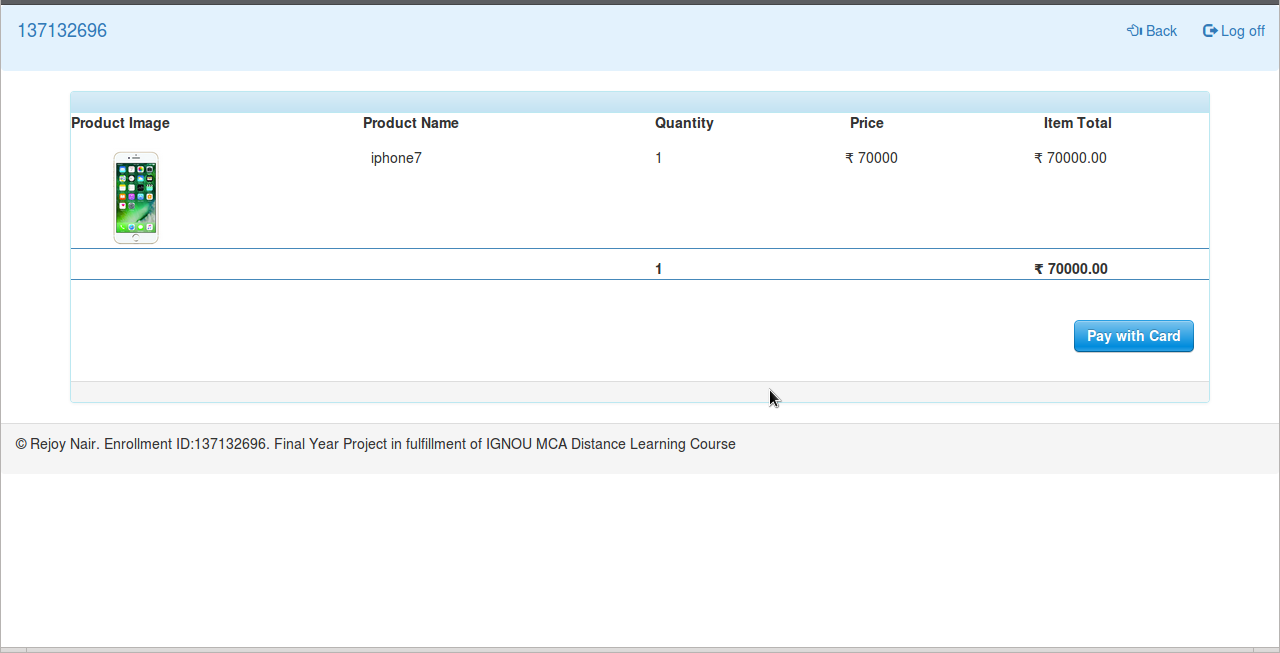
\includegraphics[ width=\textheight , keepaspectratio ]{./Images/PlaceOrderScreen.png}\\[-1em]
		%\vspace{0.25cm}
		\captionof{figure}{Customer Place Order Screen}
		\label{fig:2}
		\end{minipage}
\end{sideways}


\begin{center}
	{
	\setlength{\extrarowheight}{2pt}

	\newcolumntype{b}{X}
	\newcolumntype{s}{>{\hsize=.4\hsize}X}
	\newcolumntype{t}{>{\hsize=1.3\hsize}X}
		
	%\renewcommand\thetable{2} 					
	%\captionof{table}{ \textbf {\small {Customer Place Order Screen}}} \label{table:2}
	\vspace{0.25cm}
									
	\begin{tabularx}{\textwidth}{ | >{\ttfamily\raggedright\arraybackslash} s 
	| >{\ttfamily\raggedright\arraybackslash} t 
	| >{\ttfamily\raggedright\arraybackslash} t | }
	
	\caption{ \textbf {\small {Customer Place Order Screen}}} \\							
	\hline
								
	{\textbf{\textcolor{black}{{Sr. No.} \newline}}} & {\textbf{\textcolor{black}{{Input Element}}}} & \textbf{\textcolor{black}{{Description \& Behaviour}}} \\
								
	\hline
	1.0 & Product Image & Image of the Product added to the shopping cart \\
	\hline		
	2.0 & Product Name & Name of the Product added to the shopping cart \\
	\hline	  	 
	3.0 & Quantity & Input number box to increase or decrease the quantity of the product added to the shopping cart  \\
	\hline	  	 	
	4.0 & Price & Price of the product added to the shopping cart  \\
	\hline	  	 
	5.0 & Item Total & Total cost per line item  \\
	\hline	  
	6.0 & Total Count & Total count of products added to shopping cart \\
	\hline			 		
	7.0 & Grand Total & Total Order value  \\
	\hline	
	8.0 & Pay with Card & Button to call the Stripe`s \Gls{Payment Gateway} \gls{API}   \\
	\hline	
	9.0 & Back Button & Button to go back to the previous page i.e. the main view \\
	\hline		
	10.0 & Logoff Button & Button to logoff from the customer web portal \\
	\hline				
	\end{tabularx}
	}
\end{center}


\begin{sideways}
    \centering
		\begin{minipage}{\textheight}
		\centering
		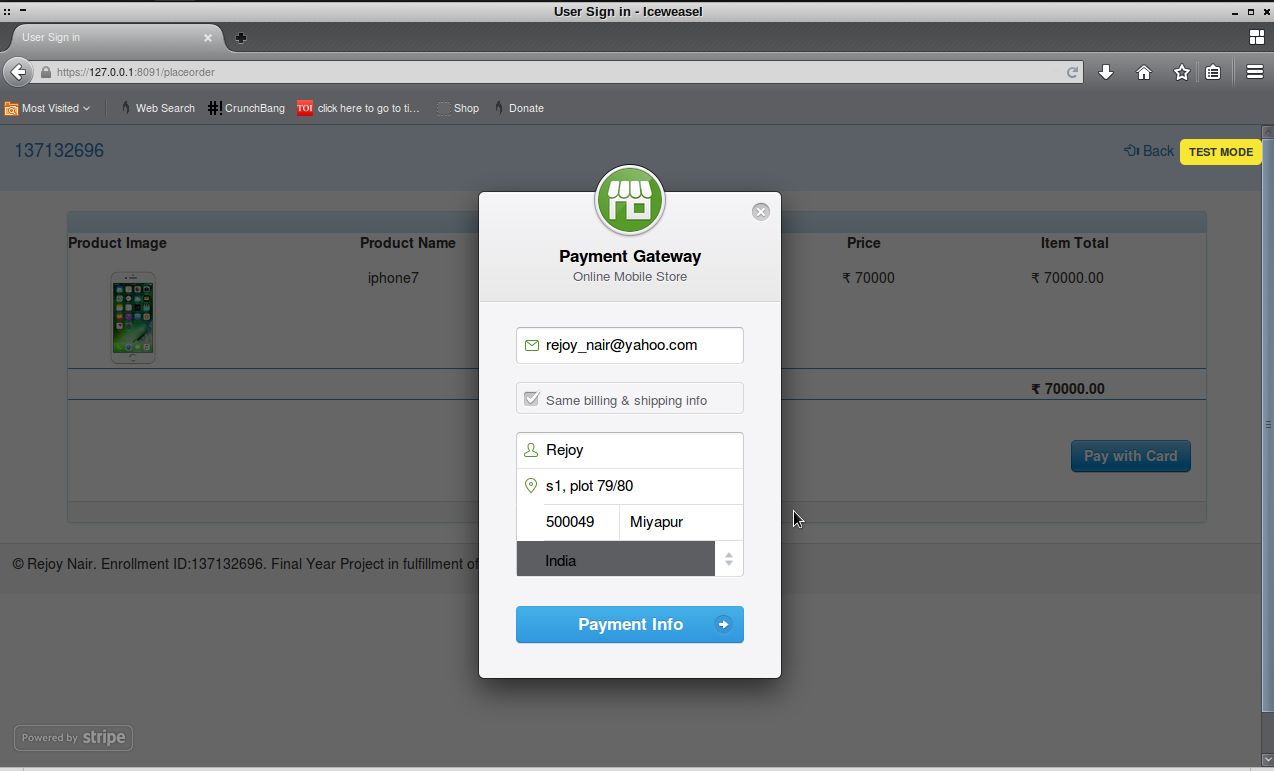
\includegraphics[ width=0.86\textheight , keepaspectratio ]{./Images/PaymentGateway1.png}\\[-1em]
		%\vspace{0.25cm}
		\captionof{figure}{Stripe Payment Gateway Submit Form-1}
		\label{fig:2}
		\end{minipage}
\end{sideways}


\begin{center}
	{
	\setlength{\extrarowheight}{2pt}

	\newcolumntype{b}{X}
	\newcolumntype{s}{>{\hsize=.4\hsize}X}
	\newcolumntype{t}{>{\hsize=1.3\hsize}X}
		
	%\renewcommand\thetable{2} 					
	%\captionof{table}{ \textbf {\small {Stripe Payment Gateway Submit Form-1}}} \label{table:2}
	\vspace{0.25cm}
									
	\begin{tabularx}{\textwidth}{ | >{\ttfamily\raggedright\arraybackslash} s 
	| >{\ttfamily\raggedright\arraybackslash} t 
	| >{\ttfamily\raggedright\arraybackslash} t | }
	
	\caption{ \textbf {\small {Stripe Payment Gateway Submit Form-1}}}	\\						
	\hline
								
	{\textbf{\textcolor{black}{{Sr. No.} \newline}}} & {\textbf{\textcolor{black}{{Input Element}}}} & \textbf{\textcolor{black}{{Description \& Behaviour}}} \\
								
	\hline
	1.0 & Label & Label on top of the form \\
	\hline		
	2.0 & Email Address & Email Address of the card Holder. This can be different from the registered email address of the customer \\
	\hline		
	3.0 & Checkbox - Billing and Shipping info & Checkbox to indicate if the billing and shipping addresses are one and the same. Default is checked. \\
	\hline	  	 
	4.0 & Name of the Card Holder & Text box to enter the name of the card holder  \\
	\hline	  	 	
	5.0 & Address Line 1 & Text box to enter the address line of the card holder  \\
	\hline	  	 
	6.0 & Pincode & Text box to enter the pincode corresponding to the address of the card holder  \\
	\hline	  	 	
	7.0 & Town / City Name & Town / city name for the entered pincode. This field is auto-populated based on the entered pincode.  \\
	\hline	  
	8.0 & Payment Info & Button to navigate to the next section of the form where the card information shall be sought \\
	\hline			 		
	9.0 & Grand Total & Total Order value  \\
	\hline	
	10.0 & Pay with Card & Button to call the Stripe`s \Gls{Payment Gateway} \Gls{API}   \\
	\hline	
	11.0 & Card Number & Text box to enter the card number of the card holder\\
	\hline		
	12.0 & Card Expiry date & Calendar widget to enter the card number of the card holder\\
	\hline				
	13.0 & Card CVV Number & Input box to enter the CVV number associated with the Card Number of the card holder\\
	\hline		
	14.0 & `Remember me` Checkbox & Checkbox to save the cardholder and the card details on Stripe`s server\\
	\hline	
	15.0 & Pay & Button to post card holder information and card details to Stripe`s server\\
	\hline										
	\end{tabularx}
	}
\end{center}


\begin{sideways}
    \centering
		\begin{minipage}{\textheight}
		\centering
		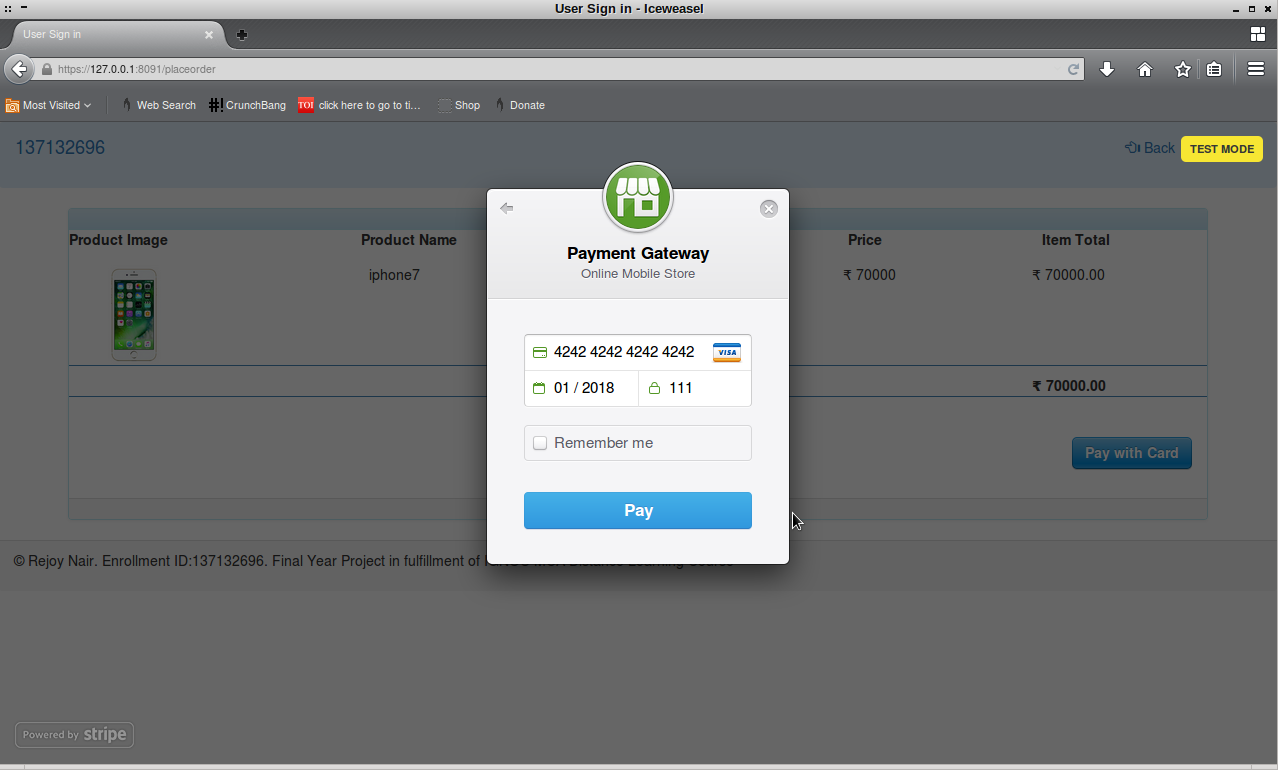
\includegraphics[ width=0.86\textheight , keepaspectratio ]{./Images/PaymentGateway2.png}\\[-1em]
		%\vspace{0.25cm}
		\captionof{figure}{Stripe Payment Gateway Submit Form-2}
		\label{fig:2}
		\end{minipage}
\end{sideways}


\begin{sideways}
    \centering
		\begin{minipage}{\textheight}
		\centering
		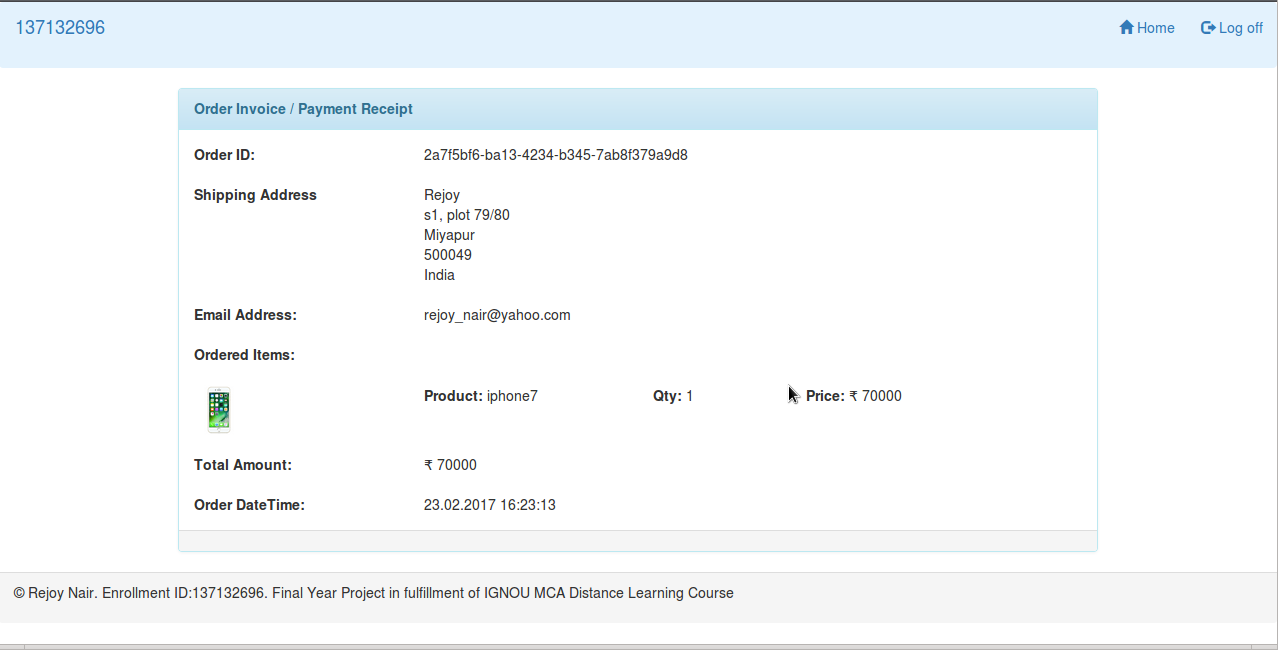
\includegraphics[ width=\textheight , keepaspectratio ]{./Images/OrderConfirmation.png}\\[-1em]
		%\vspace{0.25cm}
		\captionof{figure}{Order Confirmation Screen}
		\label{fig:2}
		\end{minipage}
\end{sideways}


\begin{center}
	{
	\setlength{\extrarowheight}{2pt}

	\newcolumntype{b}{X}
	\newcolumntype{s}{>{\hsize=.4\hsize}X}
	\newcolumntype{t}{>{\hsize=1.3\hsize}X}
		
	%\renewcommand\thetable{2} 					
	%\captionof{table}{ \textbf {\small {Order Invoice / Payment Receipt}}} \label{table:2}
	\vspace{0.25cm}
									
	\begin{tabularx}{\textwidth}{ | >{\ttfamily\raggedright\arraybackslash} s 
	| >{\ttfamily\raggedright\arraybackslash} t 
	| >{\ttfamily\raggedright\arraybackslash} t | }
	
	\caption{ \textbf {\small {Order Invoice / Payment Receipt}}}	\\						
	\hline
								
	{\textbf{\textcolor{black}{{Sr. No.} \newline}}} & {\textbf{\textcolor{black}{{Input Element}}}} & \textbf{\textcolor{black}{{Description \& Behaviour}}} \\
								
	\hline
	1.0 & Order ID & Output text displaying the Order ID field value of the Order Invoice cum payment receipt of the Order placed by the customer  \\
	\hline		
	2.0 & Shipping Address & Output text displaying the Shipping Address field value of the Order Invoice cum payment receipt of the Order placed by the customer \\
	\hline	  	 
	3.0 & Email Address & Output text displaying the Cardholder`s Email Address field value of the Order Invoice cum payment receipt of the Order placed by the customer  \\
	\hline	  	 	
	4.0 & Ordered Items - Product Image & Image of the Ordered Product corresponding to the Order Invoice cum payment receipt of the Order placed by the customer  \\
	\hline	  	 
	5.0 & Ordered Items - Product Name & Output text displaying the Name of the Ordered Product corresponding to the Order Invoice cum payment receipt of the Order placed by the customer  \\
	\hline	  
	6.0 & Ordered Items - Ordered Quantity & Output text displaying the Quantity of the Ordered Product corresponding to the Order Invoice cum payment receipt of the Order placed by the customer \\
	\hline			 		
	7.0 & Ordered Items - Amount & Output text displaying the Per Unit Cost of the Ordered Product corresponding to the Order Invoice cum payment receipt of the Order placed by the customer  \\
	\hline	
	8.0 & Total Amount & Output text displaying the Total Order Amount corresponding to the Order Invoice cum payment receipt of the Order placed by the customer  \\
	\hline	
	9.0 & Order DateTime &  Output text displaying the local date-time corresponding to the Order Invoice cum payment receipt of the Order placed by the customer \\
	\hline	
	10.0 & Home Button & Button to navigate the customer back to the main page of the customer web portal \\
	\hline					
	11.0 & Logoff Button & Button to logoff from the customer web portal \\
	\hline				
	\end{tabularx}
	}
\end{center}


\begin{sideways}
    \centering
		\begin{minipage}{\textheight}
		\centering
		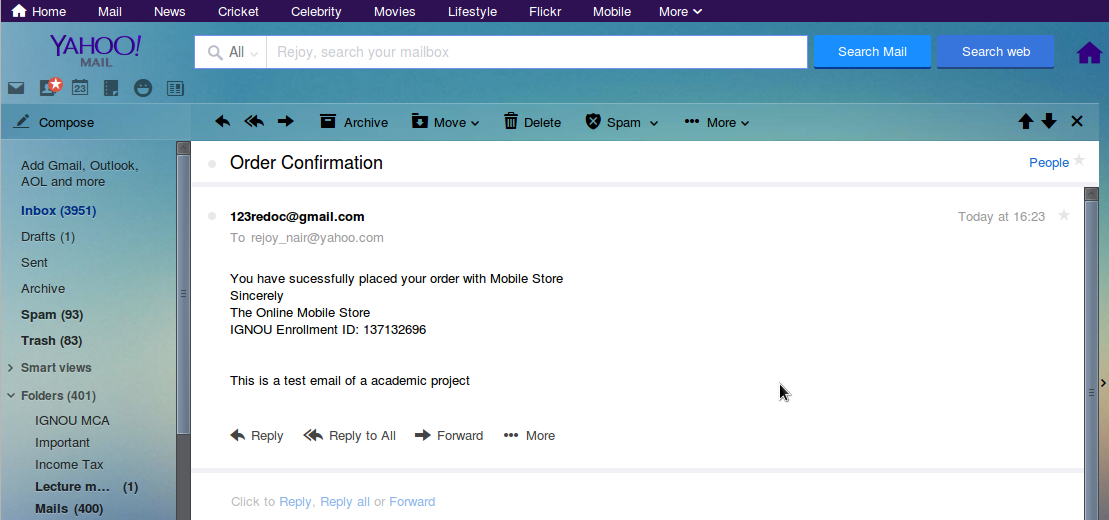
\includegraphics[ width=\textheight , keepaspectratio ]{./Images/Email.png}\\[-1em]
		%\vspace{0.25cm}
		\captionof{figure}{Email Notification in Inbox }
		\label{fig:2}
		\end{minipage}
\end{sideways}


\begin{sideways}
    \centering
		\begin{minipage}{\textheight}
		\centering
		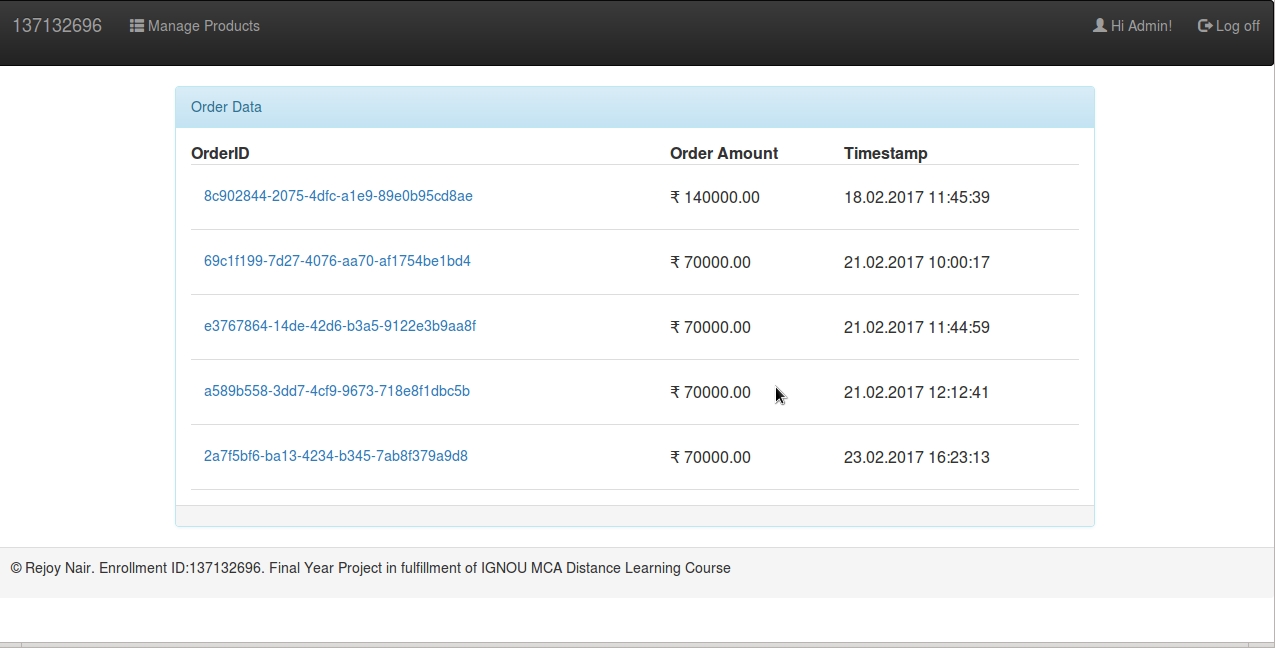
\includegraphics[ width=\textheight , keepaspectratio ]{./Images/AdminmainScreen.png}\\[-1em]
		%\vspace{0.25cm}
		\captionof{figure}{Admin User Main View}
		\label{fig:2}
		\end{minipage}
\end{sideways}


\begin{center}
	{
	\setlength{\extrarowheight}{2pt}

	\newcolumntype{b}{X}
	\newcolumntype{s}{>{\hsize=.4\hsize}X}
	\newcolumntype{t}{>{\hsize=1.3\hsize}X}
		
	%\renewcommand\thetable{2} 					
	%\captionof{table}{ \textbf {\small {Admin Main View - Order data}}} \label{table:2}
	\vspace{0.25cm}
									
	\begin{tabularx}{\textwidth}{ | >{\ttfamily\raggedright\arraybackslash} s 
	| >{\ttfamily\raggedright\arraybackslash} t 
	| >{\ttfamily\raggedright\arraybackslash} t | }
	
	\caption{ \textbf {\small {Admin Main View - Order data}}} \\							
	\hline
								
	{\textbf{\textcolor{black}{{Sr. No.} \newline}}} & {\textbf{\textcolor{black}{{Input Element}}}} & \textbf{\textcolor{black}{{Description \& Behaviour}}} \\
								
	\hline
	1.0 & Banner & Banner to place the brand logo. Currently contains the enrollment ID 137132696  \\
	\hline		
	2.0 & Manage Product & Link to navigate the Admin user to the Manage Products Page \\
	\hline	  	 
	3.0 & User Profile icon & Displays the text `Admin` indicating Admin user login  \\
	\hline	  	 	
	4.0 & Log-off & Link to log-off the Admin User from the Admin User portal  \\
	\hline	  	 
	5.0 & Order Data - Order ID & Output text displaying the Order ID of the successfully placed orders displayed in the order data table  \\
	\hline	  
	6.0 & Order Data - Order Amount & Output text displaying the total amount corresponding to each order ID of the successfully placed orders displayed in the order data table  \\
	\hline			 		
	7.0 & Order Data - Timestamp & Output text displaying the timestamp corresponding to each order ID of the successfully placed orders displayed in the order data table  \\
	\hline					
	\end{tabularx}
	}
\end{center}



\begin{sideways}
    \centering
		\begin{minipage}{\textheight}
		\centering
		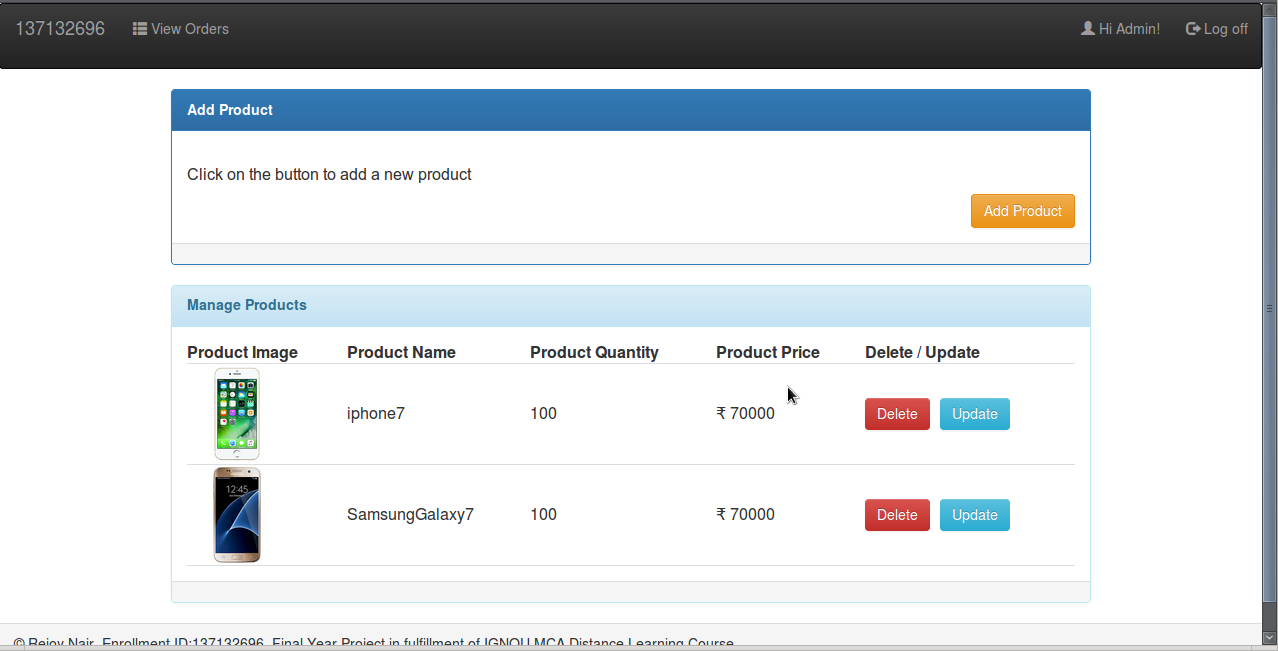
\includegraphics[ width=\textheight , keepaspectratio ]{./Images/AdminManageProduct.png}\\[-1em]
		%\vspace{0.25cm}
		\captionof{figure}{Admin - Manage Products }
		\label{fig:2}
		\end{minipage}
\end{sideways}


\begin{center}
	{
	\setlength{\extrarowheight}{2pt}

	\newcolumntype{b}{X}
	\newcolumntype{s}{>{\hsize=.4\hsize}X}
	\newcolumntype{t}{>{\hsize=1.3\hsize}X}
		
	%\renewcommand\thetable{2} 					
	%\captionof{table}{ \textbf {\small {Admin Manage Products}}} \label{table:2}
	\vspace{0.25cm}
									
	\begin{tabularx}{\textwidth}{ | >{\ttfamily\raggedright\arraybackslash} s 
	| >{\ttfamily\raggedright\arraybackslash} t 
	| >{\ttfamily\raggedright\arraybackslash} t | }
	
	\caption{ \textbf {\small {Admin Manage Products}}} \\							
	\hline
								
	{\textbf{\textcolor{black}{{Sr. No.} \newline}}} & {\textbf{\textcolor{black}{{Input Element}}}} & \textbf{\textcolor{black}{{Description \& Behaviour}}} \\
								
	\hline
	1.0 & Banner & Banner to place the brand logo. Currently contains the enrollment ID 137132696  \\
	\hline		
	2.0 & View Order & Link to navigate the Admin user back to the Admin Main View i.e., the View Order Data Page \\
	\hline	  	 
	3.0 & User Profile icon & Displays the text `Admin' indicating Admin user login  \\
	\hline	  	 	
	4.0 & Log-off & Link to log-off the Admin User from the Admin User portal  \\
	\hline	  	 
	5.0 & Add Product & Button that navigates the admin user to the add product form  \\
	\hline	  
	6.0 & Manage Products - Product Image & Image of the Product that exists in the backend database  \\
	\hline			 		
	7.0 & Manage Products - Product Name & Output text displaying the name of the Product that exists in the backend database  \\
	\hline	
	8.0 & Manage Products - Product Quantity & Output text displaying the quantity of the Product as maintained in the backend database  \\
	\hline		
	9.0 & Manage Products - Product Price & Output text displaying the price of the Product as maintained in the backend database  \\
	\hline	
	10.0 & Manage Products - Delete Button & Button to delete the record of the corresponding product from the database  \\
	\hline		
	11.0 & Manage Products - Update Button & Button to navigate the user to the update product form to update the record of the corresponding product from the database  \\
	\hline												
	\end{tabularx}
	}
\end{center}


\begin{sideways}
    \centering
		\begin{minipage}{\textheight}
		\centering
		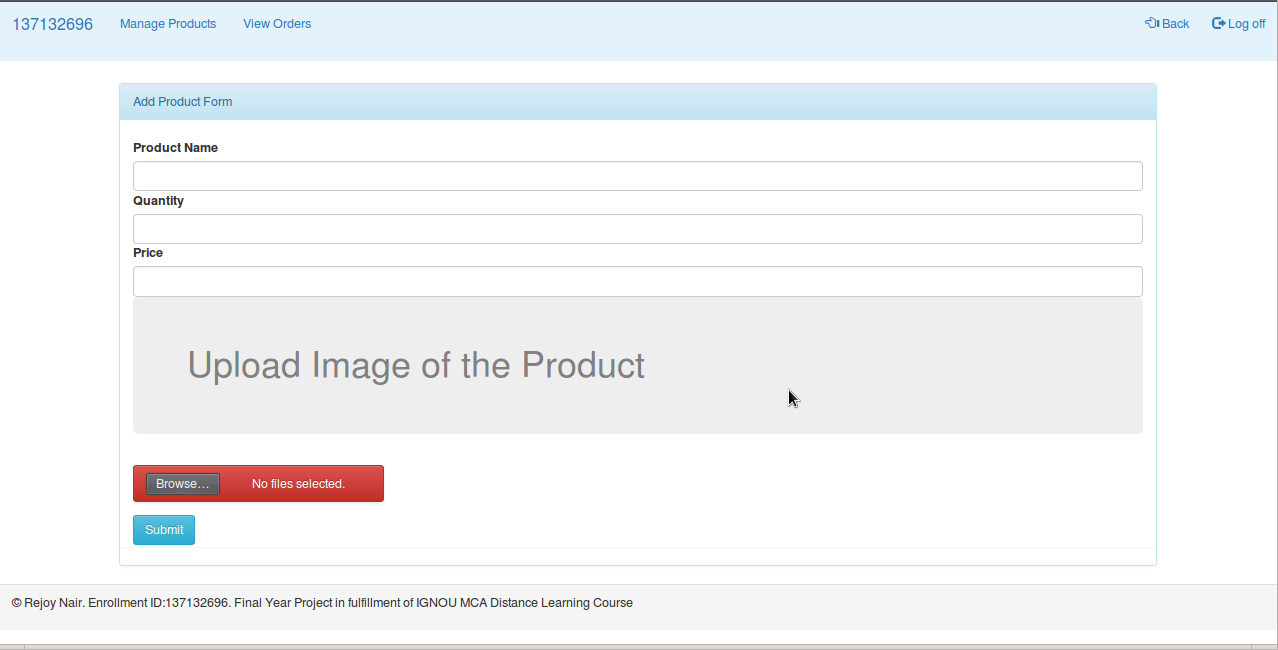
\includegraphics[ width=\textheight , keepaspectratio ]{./Images/AdminAddProductForm.png}\\[-1em]
		%\vspace{0.25cm}
		\captionof{figure}{Admin - Add Product Form}
		\label{fig:2}
		\end{minipage}
\end{sideways}


\begin{center}
	{
	\setlength{\extrarowheight}{2pt}

	\newcolumntype{b}{X}
	\newcolumntype{s}{>{\hsize=.4\hsize}X}
	\newcolumntype{t}{>{\hsize=1.3\hsize}X}
		
	%\renewcommand\thetable{2} 					
	%\captionof{table}{ \textbf {\small {Admin Manage Products}}} \label{table:2}
	\vspace{0.25cm}
									
	\begin{tabularx}{\textwidth}{ | >{\ttfamily\raggedright\arraybackslash} s 
	| >{\ttfamily\raggedright\arraybackslash} t 
	| >{\ttfamily\raggedright\arraybackslash} t | }
	
	\caption{ \textbf {\small {Admin Add Products}}} \\							
	\hline
								
	{\textbf{\textcolor{black}{{Sr. No.} \newline}}} & {\textbf{\textcolor{black}{{Input Element}}}} & \textbf{\textcolor{black}{{Description \& Behaviour}}} \\
								
	\hline
	1.0 & Banner & Banner to place the brand logo. Currently contains the enrollment ID 137132696  \\
	\hline		
	2.0 & View Order & Link to navigate the Admin user back to the Admin Main View i.e., the View Order Data Page \\
	\hline	  	 	
	3.0 & Manage Products & Link to navigate the Admin user back to the Admin - Manage Products Page \\
	\hline	  	 
	4.0 & Back Button & Navigates the admin user back to the previous page  \\
	\hline	  	 	
	4.0 & Log-off & Link to log-off the Admin User from the Admin User portal  \\
	\hline	  	 
	5.0 & Add Product - Product Name & Text field to input the name of the product to be added   \\
	\hline	  
	6.0 & Add Product - Quantity & Input field to input the name of the product to be added  \\
	\hline			 		
	7.0 & Add Product - Price & Input field to input the price of the product to be added   \\
	\hline	
	8.0 & Add Product - Upload Image File & File Upload utility to upload the image of the product to be added  \\
	\hline		
	9.0 & Add Product - Submit Button & Button to post the Add Product form details to the server  \\
	\hline	
	10.0 & Add Product - Alerts & Alerts to notify the admin users of fields that fail validation criteria  \\
	\hline		
	
	\end{tabularx}
	}
\end{center}


\begin{sideways}
    \centering
		\begin{minipage}{\textheight}
		\centering
		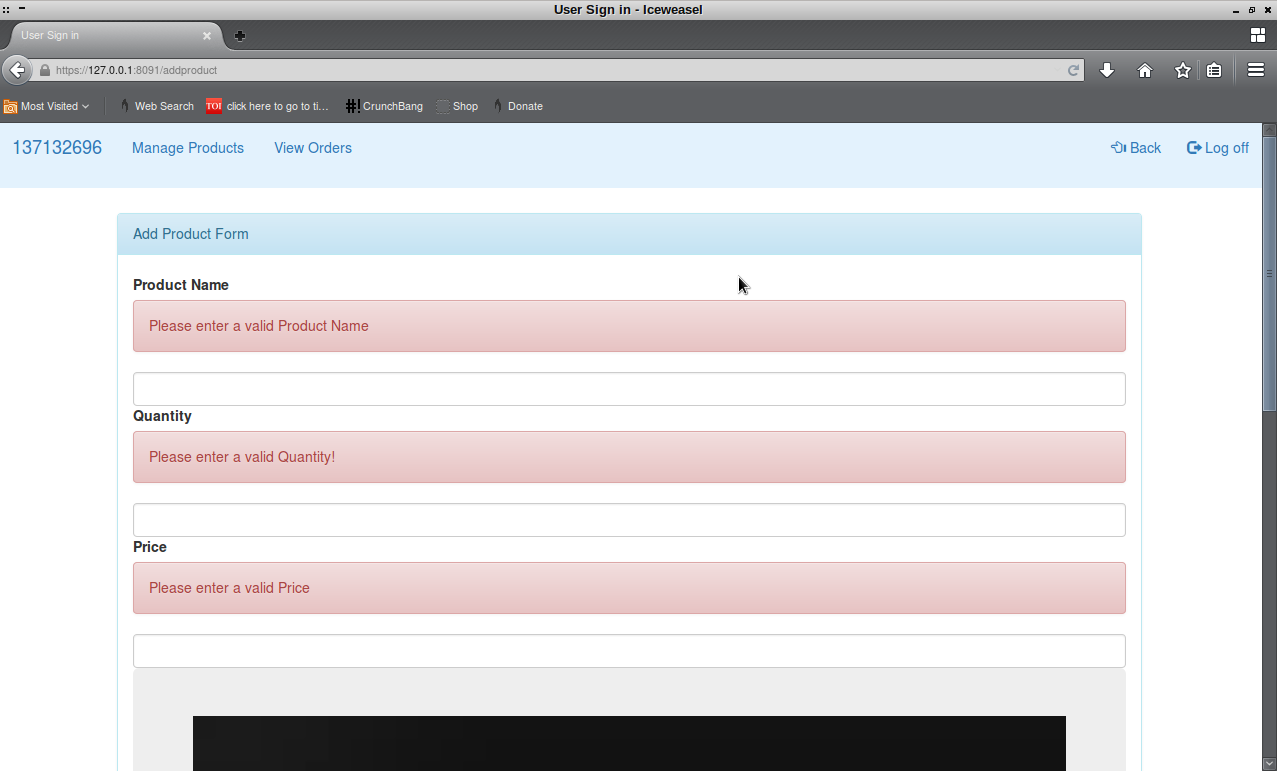
\includegraphics[ width=0.86\textheight , keepaspectratio ]{./Images/AddProdValidation1.png}\\[-1em]
		%\vspace{0.25cm}
		\captionof{figure}{Admin - Add Product Form Validations - I}
		\label{fig:2}
		\end{minipage}
\end{sideways}


\begin{sideways}
    \centering
		\begin{minipage}{\textheight}
		\centering
		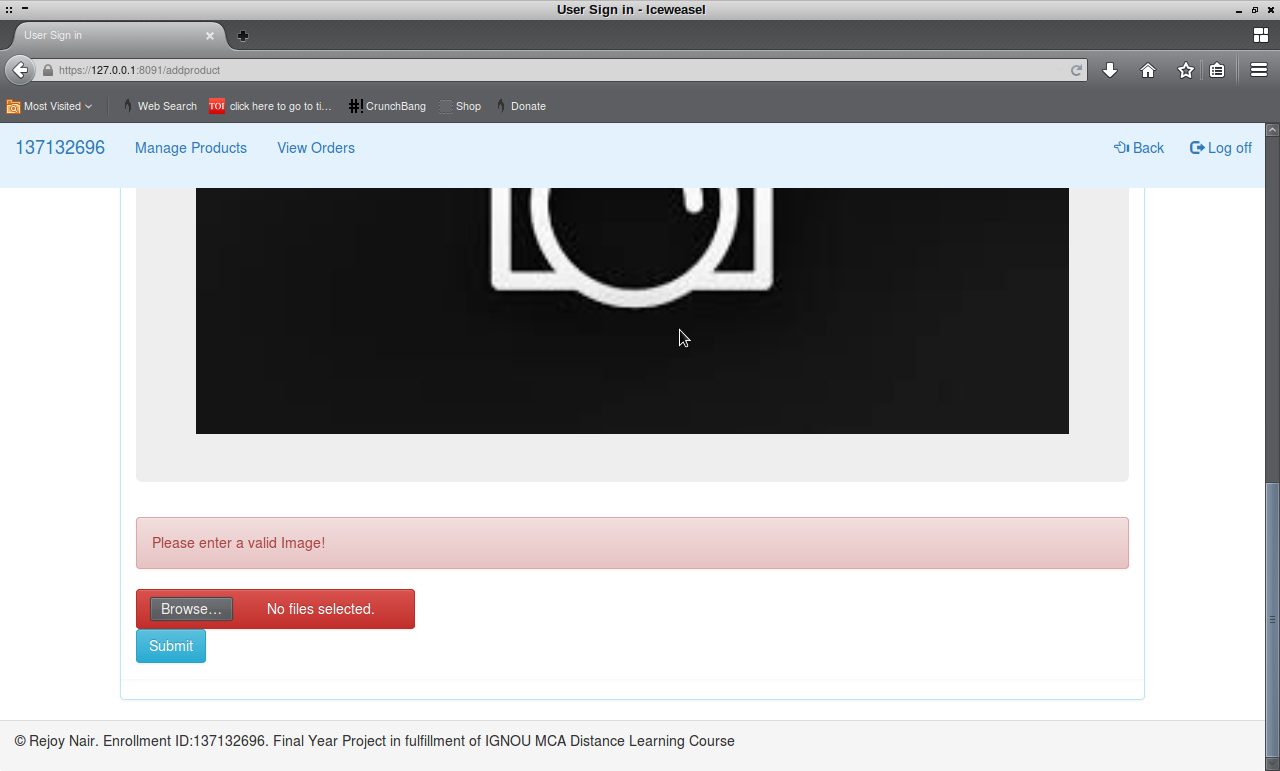
\includegraphics[ width=0.86\textheight , keepaspectratio ]{./Images/AddProdValidation2.png}\\[-1em]
		%\vspace{0.25cm}
		\captionof{figure}{Admin - Add Product Form Validation -II}
		\label{fig:2}
		\end{minipage}
\end{sideways}

\newpage

%*******************************************SECTION**********************************
\section{\MakeUppercase{Coding}}

\subsection{Go Code}

%\lstinputlisting[language=Go, firstline=37, lastline=45]{email.go}[style=Go]

\lstinputlisting[language=go,style=go]{./source/main.go}
\newpage

\lstinputlisting[language=go,style=go]{./source/data.go}
\newpage

\lstinputlisting[language=go,style=go]{./source/cookie.go}
\newpage

\lstinputlisting[language=go,style=go]{./source/product.go}
\newpage

\lstinputlisting[language=go,style=go]{./source/order.go}
\newpage

\lstinputlisting[language=go,style=go]{./source/email.go}
\newpage

\subsection{HTML Code}

\lstinputlisting[style=htmlcssjs]{./source/index.html}
\newpage

\lstinputlisting[style=htmlcssjs]{./source/main.html}
\newpage

\lstinputlisting[style=htmlcssjs]{./source/signup.html}
\newpage

\lstinputlisting[style=htmlcssjs]{./source/internal.html}
\newpage

\lstinputlisting[style=htmlcssjs]{./source/placeorder.html}
\newpage

\lstinputlisting[style=htmlcssjs]{./source/payment.html}
\newpage

\lstinputlisting[style=htmlcssjs]{./source/admin.html}
\newpage

\lstinputlisting[style=htmlcssjs]{./source/vieworder.html}
\newpage

\lstinputlisting[style=htmlcssjs]{./source/manageproduct.html}
\newpage

\lstinputlisting[style=htmlcssjs]{./source/addproduct.html}
\newpage

\lstinputlisting[style=htmlcssjs]{./source/deleteproduct.html}
\newpage

\lstinputlisting[style=htmlcssjs]{./source/showproduct.html}
\newpage

\subsection{Javascript Code}

\lstinputlisting[style=htmlcssjs]{./source/shoppingCart.js}
\newpage

\subsection{Test Cases and Test Results}

\begin{center}
	{
	\setlength{\extrarowheight}{2pt}

	\newcolumntype{b}{X}
	\newcolumntype{s}{>{\hsize=.4\hsize}X}
	\newcolumntype{t}{>{\hsize=1.3\hsize}X}
		
	%\renewcommand\thetable{2} 					
	%\captionof{table}{ \textbf {\small {Test Cases for Req. ID \ref{Signup:1} }}} \label{table:2}
	\vspace{0.25cm}
									
	\begin{tabularx}{\textwidth}{ | >{\ttfamily\raggedright\arraybackslash} s 
	| >{\ttfamily\raggedright\arraybackslash} t 
	| >{\ttfamily\raggedright\arraybackslash} t | }
	
	\caption{ \textbf {\small {Test Cases for Req. ID \ref{Signup:1} }}} \\							
	\hline
								
	{\textbf{\textcolor{black}{{Sr. No} \newline}}} & {\textbf{\textcolor{black}{{Test Cases}}}} & \textbf{\textcolor{black}{{Expected Behavior \& Status}}} \\
								
	\hline
	1.0 & Enter website URL & User should be directed to secure HTTPS connection. User should provide security certificate details. \newline \newline Pass  \\
	\hline			
	2.0 & Click on `Sign-up' link on the landing page & User should be directed to Sign-up form page. \newline \newline Pass  \\
	\hline			
	
	\end{tabularx}
	}
\end{center}


\begin{center}
	{
	\setlength{\extrarowheight}{2pt}

	\newcolumntype{b}{X}
	\newcolumntype{s}{>{\hsize=.4\hsize}X}
	\newcolumntype{t}{>{\hsize=1.3\hsize}X}
		
	%\renewcommand\thetable{2} 					
	%\captionof{table}{ \textbf {\small {Test Cases for Req. ID \ref{Signup:2} }}} \label{table:2}
	\vspace{0.25cm}
									
	\begin{tabularx}{\textwidth}{ | >{\ttfamily\raggedright\arraybackslash} s 
	| >{\ttfamily\raggedright\arraybackslash} t 
	| >{\ttfamily\raggedright\arraybackslash} t | }
	
	\caption{ \textbf {\small {Test Cases for Req. ID \ref{Signup:2} }}} \\							
	\hline
								
	{\textbf{\textcolor{black}{{Sr. No} \newline}}} & {\textbf{\textcolor{black}{{Test Cases}}}} & \textbf{\textcolor{black}{{Expected Behavior \& Status}}} \\
								
	\hline
	1.0 & Enter blank value and click on submit & Error ``Please enter a valid username'' should be received \newline \newline Pass \\
	\hline			
	2.0 & Enter a username that already exists and click on submit & Error ``Username already exists'' should be received \newline \newline Pass \\
	\hline			
	
	\end{tabularx}
	}
\end{center}

\begin{center}
	{
	\setlength{\extrarowheight}{2pt}

	\newcolumntype{b}{X}
	\newcolumntype{s}{>{\hsize=.4\hsize}X}
	\newcolumntype{t}{>{\hsize=1.3\hsize}X}
		
	%\renewcommand\thetable{2} 					
	%\captionof{table}{ \textbf {\small {Test Cases for Req. ID \ref{Signup:3} }}} \label{table:2}
	\vspace{0.25cm}
									
	\begin{tabularx}{\textwidth}{ | >{\ttfamily\raggedright\arraybackslash} s 
	| >{\ttfamily\raggedright\arraybackslash} t 
	| >{\ttfamily\raggedright\arraybackslash} t | }
	
	\caption{ \textbf {\small {Test Cases for Req. ID \ref{Signup:3} }}} \\							
	\hline
								
	{\textbf{\textcolor{black}{{Sr. No} \newline}}} & {\textbf{\textcolor{black}{{Test Cases}}}} & \textbf{\textcolor{black}{{Expected Behavior \& Status}}} \\
								
	\hline
	1.0 & Enter blank value in first name field and click on submit & Error ``Please enter a valid first name'' should be received \newline \newline Pass \\
	\hline	
	2.0 & Enter blank value in last name field and click on submit & Error ``Please enter a valid last name'' should be received \newline \newline Pass \\
	\hline	
	3.0 & Enter blank value in email address field and click on submit & Error ``Please enter a valid email address'' should be received \newline \newline Pass \\
	\hline
	4.0 & Enter a string that does not conform to the regex pattern for an email address in email address field and click on submit & Error ``Please enter a valid email address'' should be received \newline \newline Pass \\
	\hline						
	5.0 & Enter a email address that already exists and click on submit & Error ``email address already exists'' should be received	\\
	\hline
	\end{tabularx}
	}
\end{center}

\begin{center}
	{
	\setlength{\extrarowheight}{2pt}

	\newcolumntype{b}{X}
	\newcolumntype{s}{>{\hsize=.4\hsize}X}
	\newcolumntype{t}{>{\hsize=1.3\hsize}X}
		
	%\renewcommand\thetable{2} 					
	%\captionof{table}{ \textbf {\small {Test Cases for Req. ID \ref{Signup:4} }}} \label{table:2}
	\vspace{0.25cm}
									
	\begin{tabularx}{\textwidth}{ | >{\ttfamily\raggedright\arraybackslash} s 
	| >{\ttfamily\raggedright\arraybackslash} t 
	| >{\ttfamily\raggedright\arraybackslash} t | }
	
	\caption{ \textbf {\small {Test Cases for Req. ID \ref{Signup:4} }}} \\							
	\hline
								
	{\textbf{\textcolor{black}{{Sr. No} \newline}}} & {\textbf{\textcolor{black}{{Test Cases}}}} & \textbf{\textcolor{black}{{Expected Behavior \& Status}}} \\
								
	\hline
	1.0 & Enter a blank value in the password field & Error ``Please enter a valid password'' should be received \newline \newline Pass \\
	\hline			
	2.0 & Enter a blank value in the confirm password field & Error ``Please confirm your password'' should be received \newline \newline Pass \\
	\hline	
	3.0 & Enter a incorrect value in the confirm password field & Error ``Entered value does not match password'' should be received \newline \newline Pass \\
	\hline	
	\end{tabularx}
	}
\end{center}

\begin{center}
	{
	\setlength{\extrarowheight}{2pt}

	\newcolumntype{b}{X}
	\newcolumntype{s}{>{\hsize=.4\hsize}X}
	\newcolumntype{t}{>{\hsize=1.3\hsize}X}
		
	%\renewcommand\thetable{2} 					
	%\captionof{table}{ \textbf {\small {Test Cases for Req. ID \ref{Signup:5} }}} \label{table:2}
	\vspace{0.25cm}
									
	\begin{tabularx}{\textwidth}{ | >{\ttfamily\raggedright\arraybackslash} s 
	| >{\ttfamily\raggedright\arraybackslash} t 
	| >{\ttfamily\raggedright\arraybackslash} t | }
	
	\caption{ \textbf {\small {Test Cases for Req. ID \ref{Signup:5} }}} \\							
	\hline
								
	{\textbf{\textcolor{black}{{Sr. No} \newline}}} & {\textbf{\textcolor{black}{{Test Cases}}}} & \textbf{\textcolor{black}{{Expected Behavior \& Status}}} \\
								
	\hline
	1.0 & Enter invalid values in any of the fields & Error alerts should be received as described in the above test cases \newline \newline Pass \\
	\hline			
	2.0 & Enter values that are valid and click submit & Form details should be posted to the server and if accepted be committed to the database in the user table. \newline \newline Pass \\
	\hline		
	
	\end{tabularx}
	}
\end{center}

\begin{center}
	{
	\setlength{\extrarowheight}{2pt}

	\newcolumntype{b}{X}
	\newcolumntype{s}{>{\hsize=.4\hsize}X}
	\newcolumntype{t}{>{\hsize=1.3\hsize}X}
		
	%\renewcommand\thetable{2} 					
	%\captionof{table}{ \textbf {\small {Test Cases for Req. ID \ref{login:1} }}} \label{table:2}
	\vspace{0.25cm}
									
	\begin{tabularx}{\textwidth}{ | >{\ttfamily\raggedright\arraybackslash} s 
	| >{\ttfamily\raggedright\arraybackslash} t 
	| >{\ttfamily\raggedright\arraybackslash} t | }
	
	\caption{ \textbf {\small {Test Cases for Req. ID \ref{login:1} }}} \\							
	\hline
								
	{\textbf{\textcolor{black}{{Sr. No} \newline}}} & {\textbf{\textcolor{black}{{Test Cases}}}} & \textbf{\textcolor{black}{{Expected Behavior \& Status}}} \\
								
	\hline
	1.0 & At the login screen disable HTTPS in the browser settings. Try to login by entering valid username and password & Error should be received. \newline \newline Pass  \\
	\hline			
	
	\end{tabularx}
	}
\end{center}

\begin{center}
	{
	\setlength{\extrarowheight}{2pt}

	\newcolumntype{b}{X}
	\newcolumntype{s}{>{\hsize=.4\hsize}X}
	\newcolumntype{t}{>{\hsize=1.3\hsize}X}
		
	%\renewcommand\thetable{2} 					
	%\captionof{table}{ \textbf {\small {Test Cases for Req. ID \ref{login:2} }}} \label{table:2}
	\vspace{0.25cm}
									
	\begin{tabularx}{\textwidth}{ | >{\ttfamily\raggedright\arraybackslash} s 
	| >{\ttfamily\raggedright\arraybackslash} t 
	| >{\ttfamily\raggedright\arraybackslash} t | }
	
	\caption{ \textbf {\small {Test Cases for Req. ID \ref{login:2} }}} \\							
	\hline
								
	{\textbf{\textcolor{black}{{Sr. No} \newline}}} & {\textbf{\textcolor{black}{{Test Cases}}}} & \textbf{\textcolor{black}{{Expected Behavior \& Status}}} \\
								
	\hline
	1.0 & Leave the username field blank and try to login & Error ``Username or password field are empty'' should be received \newline \newline Pass  \\
	\hline		
	2.0 & Leave the password field blank and try to login & Error ``Username or password field are empty'' should be received \newline \newline Pass  \\
	\hline	
	3.0 & Enter incorrect username or password and try to login & Error ``Invalid username or password'' should be received \newline \newline Pass  \\
	\hline	
	4.0 & Enter correct username and password and try to login & User should be able to login. New Session ID unique for the username should get created. \newline \newline Pass  \\
	\hline					
	
	\end{tabularx}
	}
\end{center}

\begin{center}
	{
	\setlength{\extrarowheight}{2pt}

	\newcolumntype{b}{X}
	\newcolumntype{s}{>{\hsize=.4\hsize}X}
	\newcolumntype{t}{>{\hsize=1.3\hsize}X}
		
	%\renewcommand\thetable{2} 					
	%\captionof{table}{ \textbf {\small {Test Cases for Req. ID \ref{login:3} }}} \label{table:2}
	\vspace{0.25cm}
									
	\begin{tabularx}{\textwidth}{ | >{\ttfamily\raggedright\arraybackslash} s 
	| >{\ttfamily\raggedright\arraybackslash} t 
	| >{\ttfamily\raggedright\arraybackslash} t | }
	
	\caption{ \textbf {\small {Test Cases for Req. ID \ref{login:3} }}} \\							
	\hline
								
	{\textbf{\textcolor{black}{{Sr. No} \newline}}} & {\textbf{\textcolor{black}{{Test Cases}}}} & \textbf{\textcolor{black}{{Expected Behavior \& Status}}} \\
								
	\hline
	1.0 & Enter invalid values in any of the fields &  Error alerts should be received as described in the above test cases \newline \newline Pass  \\
	\hline			
	
	\end{tabularx}
	}
\end{center}

\begin{center}
	{
	\setlength{\extrarowheight}{2pt}

	\newcolumntype{b}{X}
	\newcolumntype{s}{>{\hsize=.4\hsize}X}
	\newcolumntype{t}{>{\hsize=1.3\hsize}X}
		
	%\renewcommand\thetable{2} 					
	%\captionof{table}{ \textbf {\small {Test Cases for Req. ID \ref{Prodlist:1} }}} \label{table:2}
	\vspace{0.25cm}
									
	\begin{tabularx}{\textwidth}{ | >{\ttfamily\raggedright\arraybackslash} s 
	| >{\ttfamily\raggedright\arraybackslash} t 
	| >{\ttfamily\raggedright\arraybackslash} t | }
	
	\caption{ \textbf {\small {Test Cases for Req. ID \ref{Prodlist:1} }}} \\							
	\hline
								
	{\textbf{\textcolor{black}{{Sr. No} \newline}}} & {\textbf{\textcolor{black}{{Test Cases}}}} & \textbf{\textcolor{black}{{Expected Behavior \& Status}}} \\
								
	\hline
	1.0 & After login, user should be presented the product listings page. All listing should be presented in the main view. & All products in the product catalog are listed and include image, name and price of the product. \newline \newline Pass  \\
	\hline	
	
	\end{tabularx}
	}
\end{center}

\begin{center}
	{
	\setlength{\extrarowheight}{2pt}

	\newcolumntype{b}{X}
	\newcolumntype{s}{>{\hsize=.4\hsize}X}
	\newcolumntype{t}{>{\hsize=1.3\hsize}X}
		
	%\renewcommand\thetable{2} 					
	%\captionof{table}{ \textbf {\small {Test Cases for Req. ID \ref{Prodlist:2} }}} \label{table:2}
	\vspace{0.25cm}
									
	\begin{tabularx}{\textwidth}{ | >{\ttfamily\raggedright\arraybackslash} s 
	| >{\ttfamily\raggedright\arraybackslash} t 
	| >{\ttfamily\raggedright\arraybackslash} t | }
	
	\caption{ \textbf {\small {Test Cases for Req. ID \ref{Prodlist:2} }}} \\							
	\hline
								
	{\textbf{\textcolor{black}{{Sr. No} \newline}}} & {\textbf{\textcolor{black}{{Test Cases}}}} & \textbf{\textcolor{black}{{Expected Behavior \& Status}}} \\
								
	\hline
	1.0 & Type a search string to match a product by its name in the search box. & All products with the name that match the description criteria shall be displayed \newline \newline Pass  \\
	\hline					
	
	\end{tabularx}
	}
\end{center}

\begin{center}
	{
	\setlength{\extrarowheight}{2pt}

	\newcolumntype{b}{X}
	\newcolumntype{s}{>{\hsize=.4\hsize}X}
	\newcolumntype{t}{>{\hsize=1.3\hsize}X}
		
	%\renewcommand\thetable{2} 					
	%\captionof{table}{ \textbf {\small {Test Cases for Req. ID \ref{Prodlist:3} }}} \label{table:2}
	\vspace{0.25cm}
									
	\begin{tabularx}{\textwidth}{ | >{\ttfamily\raggedright\arraybackslash} s 
	| >{\ttfamily\raggedright\arraybackslash} t 
	| >{\ttfamily\raggedright\arraybackslash} t | }
	
	\caption{ \textbf {\small {Test Cases for Req. ID \ref{Prodlist:3} }}} \\							
	\hline
								
	{\textbf{\textcolor{black}{{Sr. No} \newline}}} & {\textbf{\textcolor{black}{{Test Cases}}}} & \textbf{\textcolor{black}{{Expected Behavior \& Status}}} \\
								
	\hline
	1.0 & Select any new product on the listings page and add it to the shopping cart by clicking on the button & Product should get added to the shopping cart list. \newline \newline Local storage object should be created. \newline \newline Pass  \\
	\hline	
	2.0 & Select any product on the listings page that has already been added to the shopping cart and add it again by clicking on the button & Quantity of the listed Product should get incremented by 1 unit. \newline \newline Local storage object should modified accordingly. \newline \newline Pass  \\
	\hline			
	
	\end{tabularx}
	}
\end{center}

\newpage
\begin{center}
	{
	\setlength{\extrarowheight}{2pt}

	\newcolumntype{b}{X}
	\newcolumntype{s}{>{\hsize=.4\hsize}X}
	\newcolumntype{t}{>{\hsize=1.3\hsize}X}
		
	%\renewcommand\thetable{2} 					
	%\captionof{table}{ \textbf {\small {Test Cases for Req. ID \ref{Shcart:1} }}} \label{table:2}
	\vspace{0.25cm}
									
	\begin{tabularx}{\textwidth}{ | >{\ttfamily\raggedright\arraybackslash} s 
	| >{\ttfamily\raggedright\arraybackslash} t 
	| >{\ttfamily\raggedright\arraybackslash} t | }
	
	\caption{ \textbf {\small {Test Cases for Req. ID \ref{Shcart:1} }}} \\							
	\hline
								
	{\textbf{\textcolor{black}{{Sr. No} \newline}}} & {\textbf{\textcolor{black}{{Test Cases}}}} & \textbf{\textcolor{black}{{Expected Behavior \& Status}}} \\
								
	\hline
	1.0 & Add a product to the shopping cart & Display count of the shopping cart should increase by 1. \newline \newline Product details that include the image, quantity being added, price per unit and the total cost for the selected product should be displayed in the shopping cart dropdown list \newline \newline Pass  \\
	\hline			
	
	\end{tabularx}
	}
\end{center}

\begin{center}
	{
	\setlength{\extrarowheight}{2pt}

	\newcolumntype{b}{X}
	\newcolumntype{s}{>{\hsize=.4\hsize}X}
	\newcolumntype{t}{>{\hsize=1.3\hsize}X}
		
	%\renewcommand\thetable{2} 					
	%\captionof{table}{ \textbf {\small {Test Cases for Req. ID \ref{Shcart:2} }}} \label{table:2}
	\vspace{0.25cm}
									
	\begin{tabularx}{\textwidth}{ | >{\ttfamily\raggedright\arraybackslash} s 
	| >{\ttfamily\raggedright\arraybackslash} t 
	| >{\ttfamily\raggedright\arraybackslash} t | }
	
	\caption{ \textbf {\small {Test Cases for Req. ID \ref{Shcart:2} }}} \\							
	\hline
								
	{\textbf{\textcolor{black}{{Sr. No} \newline}}} & {\textbf{\textcolor{black}{{Test Cases}}}} & \textbf{\textcolor{black}{{Expected Behavior \& Status}}} \\
								
	\hline
	1.0 & In the shopping cart dropdown list, change the quantity by using the number input control  & Minimum value to which the quantity can be reduced is 1 \newline \newline Total product cost should change accordingly \newline \newline Pass   \\
	\hline
	2.0 & In the shopping cart dropdown list, click on the `+' button in the last column  & Total product quantity should increase by 1 unit \newline \newline Total product cost should change accordingly \newline \newline Pass   \\	
	\hline	
	3.0 & In the shopping cart dropdown list, click on the `-' button in the last column  & Total product quantity should decrease by 1 unit \newline \newline Total product cost should change accordingly \newline \newline Pass   \\	
	\hline				
	
	\end{tabularx}
	}
\end{center}

\begin{center}
	{
	\setlength{\extrarowheight}{2pt}

	\newcolumntype{b}{X}
	\newcolumntype{s}{>{\hsize=.4\hsize}X}
	\newcolumntype{t}{>{\hsize=1.3\hsize}X}
		
	%\renewcommand\thetable{2} 					
	%\captionof{table}{ \textbf {\small {Test Cases for Req. ID \ref{Shcart:3} }}} \label{table:2}
	\vspace{0.25cm}
									
	\begin{tabularx}{\textwidth}{ | >{\ttfamily\raggedright\arraybackslash} s 
	| >{\ttfamily\raggedright\arraybackslash} t 
	| >{\ttfamily\raggedright\arraybackslash} t | }
	
	\caption{ \textbf {\small {Test Cases for Req. ID \ref{Shcart:3} }}} \\							
	\hline
								
	{\textbf{\textcolor{black}{{Sr. No} \newline}}} & {\textbf{\textcolor{black}{{Test Cases}}}} & \textbf{\textcolor{black}{{Expected Behavior \& Status}}} \\
								
	\hline
	1.0 & Add a product to the shopping cart and change its quantity to different values  & Total cost cannot be zero. \newline \newline Total Cost = Quantity * Price per unit \newline \newline Pass  \\
	\hline			
	
	\end{tabularx}
	}
\end{center}

\begin{center}
	{
	\setlength{\extrarowheight}{2pt}

	\newcolumntype{b}{X}
	\newcolumntype{s}{>{\hsize=.4\hsize}X}
	\newcolumntype{t}{>{\hsize=1.3\hsize}X}
		
	%\renewcommand\thetable{2} 					
	%\captionof{table}{ \textbf {\small {Test Cases for Req. ID \ref{Shcart:4} }}} \label{table:2}
	\vspace{0.25cm}
									
	\begin{tabularx}{\textwidth}{ | >{\ttfamily\raggedright\arraybackslash} s 
	| >{\ttfamily\raggedright\arraybackslash} t 
	| >{\ttfamily\raggedright\arraybackslash} t | }
	
	\caption{ \textbf {\small {Test Cases for Req. ID \ref{Shcart:4} }}} \\							
	\hline
								
	{\textbf{\textcolor{black}{{Sr. No} \newline}}} & {\textbf{\textcolor{black}{{Test Cases}}}} & \textbf{\textcolor{black}{{Expected Behavior \& Status}}} \\
								
	\hline
	1.0 & In the shopping cart dropdown list, click on the `X' button in the last column  & Line item for the product in the shopping cart list should get removed \newline \newline Pass   \\	
	\hline		
	
	\end{tabularx}
	}
\end{center}

\begin{center}
	{
	\setlength{\extrarowheight}{2pt}

	\newcolumntype{b}{X}
	\newcolumntype{s}{>{\hsize=.4\hsize}X}
	\newcolumntype{t}{>{\hsize=1.3\hsize}X}
		
	%\renewcommand\thetable{2} 					
	%\captionof{table}{ \textbf {\small {Test Cases for Req. ID \ref{Shcart:5} }}} \label{table:2}
	\vspace{0.25cm}
									
	\begin{tabularx}{\textwidth}{ | >{\ttfamily\raggedright\arraybackslash} s 
	| >{\ttfamily\raggedright\arraybackslash} t 
	| >{\ttfamily\raggedright\arraybackslash} t | }
	
	\caption{ \textbf {\small {Test Cases for Req. ID \ref{Shcart:5} }}}	\\						
	\hline
								
	{\textbf{\textcolor{black}{{Sr. No} \newline}}} & {\textbf{\textcolor{black}{{Test Cases}}}} & \textbf{\textcolor{black}{{Expected Behavior \& Status}}} \\
								
	\hline
	1.0 & With no products added to the shopping cart click on the `Place Order' or checkout button & Error should be received \newline \newline Pass  \\
	\hline	
	2.0 & With products added to the shopping cart click on the `Place Order' or checkout button & User should be navigated to the Place Order page \newline \newline Pass  \\
	\hline	
	3.0 & With products added to the shopping cart, disconnect the Internet connection. Then reconnect and click on the `Place Order' or checkout button & User should not be navigated to the Place Order page. User should get logged out with message for session expired. \newline \newline Pass  \\
	\hline						
	
	\end{tabularx}
	}
\end{center}


\begin{center}
	{
	\setlength{\extrarowheight}{2pt}

	\newcolumntype{b}{X}
	\newcolumntype{s}{>{\hsize=.4\hsize}X}
	\newcolumntype{t}{>{\hsize=1.3\hsize}X}
		
	%\renewcommand\thetable{2} 					
	%\captionof{table}{ \textbf {\small {Test Cases for Req. ID \ref{Plcord:1} }}} \label{table:2}
	\vspace{0.25cm}
									
	\begin{tabularx}{\textwidth}{ | >{\ttfamily\raggedright\arraybackslash} s 
	| >{\ttfamily\raggedright\arraybackslash} t 
	| >{\ttfamily\raggedright\arraybackslash} t | }
	
	\caption{ \textbf {\small {Test Cases for Req. ID \ref{Plcord:1} }}} \\							
	\hline
								
	{\textbf{\textcolor{black}{{Sr. No} \newline}}} & {\textbf{\textcolor{black}{{Test Cases}}}} & \textbf{\textcolor{black}{{Expected Behavior \& Status}}} \\
								
	\hline
	1.0 & Add products to shopping cart and checkout & Products should be listed with details i.e. the image, quantity being ordered, price per unit, total cost of the product. \newline \newline Pass  \\
	\hline			
	
	\end{tabularx}
	}
\end{center}

\begin{center}
	{
	\setlength{\extrarowheight}{2pt}

	\newcolumntype{b}{X}
	\newcolumntype{s}{>{\hsize=.4\hsize}X}
	\newcolumntype{t}{>{\hsize=1.3\hsize}X}
		
	%\renewcommand\thetable{2} 					
	%\captionof{table}{ \textbf {\small {Test Cases for Req. ID \ref{Plcord:2} }}} \label{table:2}
	\vspace{0.25cm}
									
	\begin{tabularx}{\textwidth}{ | >{\ttfamily\raggedright\arraybackslash} s 
	| >{\ttfamily\raggedright\arraybackslash} t 
	| >{\ttfamily\raggedright\arraybackslash} t | }
	
	\caption{ \textbf {\small {Test Cases for Req. ID \ref{Plcord:2} }}} \\							
	\hline
								
	{\textbf{\textcolor{black}{{Sr. No} \newline}}} & {\textbf{\textcolor{black}{{Test Cases}}}} & \textbf{\textcolor{black}{{Expected Behavior \& Status}}} \\
								
	\hline
	1.0 & Check Order basket product total cost  & Total cost cannot be zero. \newline \newline Total Cost = Quantity * Price per unit \newline \newline Pass  \\
	\hline	
	
	\end{tabularx}
	}
\end{center}

\begin{center}
	{
	\setlength{\extrarowheight}{2pt}

	\newcolumntype{b}{X}
	\newcolumntype{s}{>{\hsize=.4\hsize}X}
	\newcolumntype{t}{>{\hsize=1.3\hsize}X}
		
	%\renewcommand\thetable{2} 					
	%\captionof{table}{ \textbf {\small {Test Cases for Req. ID \ref{Plcord:3} }}} \label{table:2}
	\vspace{0.25cm}
									
	\begin{tabularx}{\textwidth}{ | >{\ttfamily\raggedright\arraybackslash} s 
	| >{\ttfamily\raggedright\arraybackslash} t 
	| >{\ttfamily\raggedright\arraybackslash} t | }
	
	\caption{ \textbf {\small {Test Cases for Req. ID \ref{Plcord:3} }}} \\							
	\hline
								
	{\textbf{\textcolor{black}{{Sr. No} \newline}}} & {\textbf{\textcolor{black}{{Test Cases}}}} & \textbf{\textcolor{black}{{Expected Behavior \& Status}}} \\
								
	\hline
	1.0 & Check Order basket overall product quantity  & Total order quantity cannot be zero. \newline \newline Total order quantity = sum of individual product quantities \newline \newline Pass  \\
	\hline		
	2.0 & Check Order basket product total order cost  & Total order cost cannot be zero. \newline \newline Total order Cost = sum of individual order cost by products added \newline \newline Pass  \\
	\hline			
	
	\end{tabularx}
	}
\end{center}

\begin{center}
	{
	\setlength{\extrarowheight}{2pt}

	\newcolumntype{b}{X}
	\newcolumntype{s}{>{\hsize=.4\hsize}X}
	\newcolumntype{t}{>{\hsize=1.3\hsize}X}
		
	%\renewcommand\thetable{2} 					
	%\captionof{table}{ \textbf {\small {Test Cases for Req. ID \ref{Plcord:4} }}} \label{table:2}
	\vspace{0.25cm}
									
	\begin{tabularx}{\textwidth}{ | >{\ttfamily\raggedright\arraybackslash} s 
	| >{\ttfamily\raggedright\arraybackslash} t 
	| >{\ttfamily\raggedright\arraybackslash} t | }
	
	\caption{ \textbf {\small {Test Cases for Req. ID \ref{Plcord:4} }}}	\\						
	\hline
								
	{\textbf{\textcolor{black}{{Sr. No} \newline}}} & {\textbf{\textcolor{black}{{Test Cases}}}} & \textbf{\textcolor{black}{{Expected Behavior \& Status}}} \\
								
	\hline
	1.0 & Click on `Pay with card' button & Clicking on button should create a call to the Stripe Payment Gateway API and present the Stripe Checkout form. \newline \newline Pass\\
	\hline		
	2.0 & At the Place Order page disconnect the Internet. Reconnect and Click on `Pay with card' button & User session should invalidated. user should get logged out with message ``your session has expired. Please Login again'' form. \newline \newline Pass \\
	\hline				
	
	\end{tabularx}
	}
\end{center}

\begin{center}
	{
	\setlength{\extrarowheight}{2pt}

	\newcolumntype{b}{X}
	\newcolumntype{s}{>{\hsize=.4\hsize}X}
	\newcolumntype{t}{>{\hsize=1.3\hsize}X}
		
	%\renewcommand\thetable{2} 					
	%\captionof{table}{ \textbf {\small {Test Cases for Req. ID \ref{Plcord:5} }}} \label{table:2}
	\vspace{0.25cm}
									
	\begin{tabularx}{\textwidth}{ | >{\ttfamily\raggedright\arraybackslash} s 
	| >{\ttfamily\raggedright\arraybackslash} t 
	| >{\ttfamily\raggedright\arraybackslash} t | }
	
	\caption{ \textbf {\small {Test Cases for Req. ID \ref{Plcord:5} }}} \\							
	\hline
								
	{\textbf{\textcolor{black}{{Sr. No} \newline}}} & {\textbf{\textcolor{black}{{Test Cases}}}} & \textbf{\textcolor{black}{{Expected Behavior \& Status}}} \\
								
	\hline
	1.0 & Click on the back button & User should be navigated back to the product listing page \newline \newline Pass  \\
	\hline			
	
	\end{tabularx}
	}
\end{center}

\begin{center}
	{
	\setlength{\extrarowheight}{2pt}

	\newcolumntype{b}{X}
	\newcolumntype{s}{>{\hsize=.4\hsize}X}
	\newcolumntype{t}{>{\hsize=1.3\hsize}X}
		
	%\renewcommand\thetable{2} 					
	%\captionof{table}{ \textbf {\small {Test Cases for Req. ID \ref{Pay:1} }}} \label{table:2}
	\vspace{0.25cm}
									
	\begin{tabularx}{\textwidth}{ | >{\ttfamily\raggedright\arraybackslash} s 
	| >{\ttfamily\raggedright\arraybackslash} t 
	| >{\ttfamily\raggedright\arraybackslash} t | }
	
	\caption{ \textbf {\small {Test Cases for Req. ID \ref{Pay:1} }}} \\							
	\hline
								
	{\textbf{\textcolor{black}{{Sr. No} \newline}}} & {\textbf{\textcolor{black}{{Test Cases}}}} & \textbf{\textcolor{black}{{Expected Behavior \& Status}}} \\
								
	\hline
	1.0 & Leave the email address field blank & Error should be received and use should not be able to complete the payment process \newline \newline Pass  \\
	\hline			
	2.0 & Enter an invalid string that does not conform to the regex pattern of an email address & Error should be received and use should not be able to complete the payment process \newline \newline Pass  \\
	\hline	
	
	\end{tabularx}
	}
\end{center}

\begin{center}
	{
	\setlength{\extrarowheight}{2pt}

	\newcolumntype{b}{X}
	\newcolumntype{s}{>{\hsize=.4\hsize}X}
	\newcolumntype{t}{>{\hsize=1.3\hsize}X}
		
	%\renewcommand\thetable{2} 					
	%\captionof{table}{ \textbf {\small {Test Cases for Req. ID \ref{Pay:2} }}} \label{table:2}
	\vspace{0.25cm}
									
	\begin{tabularx}{\textwidth}{ | >{\ttfamily\raggedright\arraybackslash} s 
	| >{\ttfamily\raggedright\arraybackslash} t 
	| >{\ttfamily\raggedright\arraybackslash} t | }
	
	\caption{ \textbf {\small {Test Cases for Req. ID \ref{Pay:2} }}} \\
								
	\hline
								
	{\textbf{\textcolor{black}{{Sr. No} \newline}}} & {\textbf{\textcolor{black}{{Test Cases}}}} & \textbf{\textcolor{black}{{Expected Behavior \& Status}}} \\
								
	\hline
	1.0 & Leave any of the required fields blank i.e \newline Address Line 1, \newline Pincode, \newline Town/City, \newline Country  & Error should be received and use should not be able to complete the payment process \newline \newline Pass  \\
	\hline			
	
	\end{tabularx}
	}
\end{center}

\begin{center}
	{
	\setlength{\extrarowheight}{2pt}

	\newcolumntype{b}{X}
	\newcolumntype{s}{>{\hsize=.4\hsize}X}
	\newcolumntype{t}{>{\hsize=1.3\hsize}X}
		
	%\renewcommand\thetable{2} 					
	%\captionof{table}{ \textbf {\small {Test Cases for Req. ID \ref{Pay:3} }}} \label{table:2}
	\vspace{0.25cm}
									
	\begin{tabularx}{\textwidth}{ | >{\ttfamily\raggedright\arraybackslash} s 
	| >{\ttfamily\raggedright\arraybackslash} t 
	| >{\ttfamily\raggedright\arraybackslash} t | }
	
	\caption{ \textbf {\small {Test Cases for Req. ID \ref{Pay:3} }}} \\
								
	\hline
								
	{\textbf{\textcolor{black}{{Sr. No} \newline}}} & {\textbf{\textcolor{black}{{Test Cases}}}} & \textbf{\textcolor{black}{{Expected Behavior \& Status}}} \\
								
	\hline
	1.0 & Leave any of the required fields blanks i.e. \newline Card Number \newline Card Expiry Date \newline Card CVV & Error should be received and use should not be able to complete the payment process \newline \newline Pass   \\
	\hline		
	2.0 & Enter a previous date value in the card expiry date field & Error should be received and use should not be able to complete the payment process \newline \newline Pass   \\		
	\hline
	
	\end{tabularx}
	}
\end{center}

\begin{center}
	{
	\setlength{\extrarowheight}{2pt}

	\newcolumntype{b}{X}
	\newcolumntype{s}{>{\hsize=.4\hsize}X}
	\newcolumntype{t}{>{\hsize=1.3\hsize}X}
		
	%\renewcommand\thetable{2} 					
	%\captionof{table}{ \textbf {\small {Test Cases for Req. ID \ref{Pay:4} }}} \label{table:2}
	\vspace{0.25cm}
									
	\begin{tabularx}{\textwidth}{ | >{\ttfamily\raggedright\arraybackslash} s 
	| >{\ttfamily\raggedright\arraybackslash} t 
	| >{\ttfamily\raggedright\arraybackslash} t | }
	
	\caption{ \textbf {\small {Test Cases for Req. ID \ref{Pay:4} }}} \\							
	\hline
								
	{\textbf{\textcolor{black}{{Sr. No} \newline}}} & {\textbf{\textcolor{black}{{Test Cases}}}} & \textbf{\textcolor{black}{{Expected Behavior \& Status}}} \\
								
	\hline
	1.0 & Click on the checkbox `Remember Me'. Make Payment for the order. Relogin and initiate another order & Next time on the payment page, the saved card details should be presented to the user. \newline \newline Pass   \\
	\hline			
	
	\end{tabularx}
	}
\end{center}

\begin{center}
	{
	\setlength{\extrarowheight}{2pt}

	\newcolumntype{b}{X}
	\newcolumntype{s}{>{\hsize=.4\hsize}X}
	\newcolumntype{t}{>{\hsize=1.3\hsize}X}
		
	%\renewcommand\thetable{2} 					
	%\captionof{table}{ \textbf {\small {Test Cases for Req. ID \ref{Pay:5} }}} \label{table:2}
	\vspace{0.25cm}
									
	\begin{tabularx}{\textwidth}{ | >{\ttfamily\raggedright\arraybackslash} s 
	| >{\ttfamily\raggedright\arraybackslash} t 
	| >{\ttfamily\raggedright\arraybackslash} t | }
	
	\caption{ \textbf {\small {Test Cases for Req. ID \ref{Pay:5} }}} \\							
	\hline
								
	{\textbf{\textcolor{black}{{Sr. No} \newline}}} & {\textbf{\textcolor{black}{{Test Cases}}}} & \textbf{\textcolor{black}{{Expected Behavior \& Status}}} \\
								
	\hline
	1.0 & Close the Stripe Payment form & User should be navigated back to the place Order page \newline \newline Pass  \\
	\hline			
	
	\end{tabularx}
	}
\end{center}

\newpage

\begin{center}
	{
	\setlength{\extrarowheight}{2pt}

	\newcolumntype{b}{X}
	\newcolumntype{s}{>{\hsize=.4\hsize}X}
	\newcolumntype{t}{>{\hsize=1.3\hsize}X}
		
	%\renewcommand\thetable{2} 					
	%\captionof{table}{ \textbf {\small {Test Cases for Req. ID \ref{Inv:1} }}} \label{table:2}
	\vspace{0.25cm}
									
	\begin{tabularx}{\textwidth}{ | >{\ttfamily\raggedright\arraybackslash} s 
	| >{\ttfamily\raggedright\arraybackslash} t 
	| >{\ttfamily\raggedright\arraybackslash} t | }
	
	\caption{ \textbf {\small {Test Cases for Req. ID \ref{Inv:1} }}} \\							
	\hline
								
	{\textbf{\textcolor{black}{{Sr. No} \newline}}} & {\textbf{\textcolor{black}{{Test Cases}}}} & \textbf{\textcolor{black}{{Expected Behavior \& Status}}} \\
								
	\hline
	1.0 & Place Order & Invoice cum payment receipt should be received and should not be empty \newline \newline Pass  \\
	\hline	
	2.0 & Place Order. Disconnect network. Reconnect & Invoice cum payment receipt should not be received as user session will be invalid \newline \newline Pass  \\
	\hline				
	
	\end{tabularx}
	}
\end{center}

\begin{center}
	{
	\setlength{\extrarowheight}{2pt}

	\newcolumntype{b}{X}
	\newcolumntype{s}{>{\hsize=.4\hsize}X}
	\newcolumntype{t}{>{\hsize=1.3\hsize}X}
		
	%\renewcommand\thetable{2} 					
	%\captionof{table}{ \textbf {\small {Test Cases for Req. ID \ref{Inv:2} }}} \label{table:2}
	\vspace{0.25cm}
									
	\begin{tabularx}{\textwidth}{ | >{\ttfamily\raggedright\arraybackslash} s 
	| >{\ttfamily\raggedright\arraybackslash} t 
	| >{\ttfamily\raggedright\arraybackslash} t | }
	
	\caption{ \textbf {\small {Test Cases for Req. ID \ref{Inv:2} }}} \\							
	\hline
								
	{\textbf{\textcolor{black}{{Sr. No} \newline}}} & {\textbf{\textcolor{black}{{Test Cases}}}} & \textbf{\textcolor{black}{{Expected Behavior \& Status}}} \\
								
	\hline
	1.0 & Place Order & Order invoice copy cum payment receipt should contain the Order ID \newline \newline Pass \\
	\hline			
	
	\end{tabularx}
	}
\end{center}
\newpage

\begin{center}
	{
	\setlength{\extrarowheight}{2pt}

	\newcolumntype{b}{X}
	\newcolumntype{s}{>{\hsize=.4\hsize}X}
	\newcolumntype{t}{>{\hsize=1.3\hsize}X}
		
	%\renewcommand\thetable{2} 					
	%\captionof{table}{ \textbf {\small {Test Cases for Req. ID \ref{Inv:3} }}} \label{table:2}
	\vspace{0.25cm}
									
	\begin{tabularx}{\textwidth}{ | >{\ttfamily\raggedright\arraybackslash} s 
	| >{\ttfamily\raggedright\arraybackslash} t 
	| >{\ttfamily\raggedright\arraybackslash} t | }
	
	\caption{ \textbf {\small {Test Cases for Req. ID \ref{Inv:3} }}} \\							
	\hline
								
	{\textbf{\textcolor{black}{{Sr. No} \newline}}} & {\textbf{\textcolor{black}{{Test Cases}}}} & \textbf{\textcolor{black}{{Expected Behavior \& Status}}} \\
								
	\hline
	1.0 & Place Order & Order invoice copy cum payment receipt should contain product details such as the image, quantity of the product ordered, price per unit of the product and the total cost of the product \newline \newline Pass \\
	\hline			
	
	\end{tabularx}
	}
\end{center}

\begin{center}
	{
	\setlength{\extrarowheight}{2pt}

	\newcolumntype{b}{X}
	\newcolumntype{s}{>{\hsize=.4\hsize}X}
	\newcolumntype{t}{>{\hsize=1.3\hsize}X}
		
	%\renewcommand\thetable{2} 					
	%\captionof{table}{ \textbf {\small {Test Cases for Req. ID \ref{Inv:4} }}} \label{table:2}
	\vspace{0.25cm}
									
	\begin{tabularx}{\textwidth}{ | >{\ttfamily\raggedright\arraybackslash} s 
	| >{\ttfamily\raggedright\arraybackslash} t 
	| >{\ttfamily\raggedright\arraybackslash} t | }
	
	\caption{ \textbf {\small {Test Cases for Req. ID \ref{Inv:4} }}} \\							
	\hline
								
	{\textbf{\textcolor{black}{{Sr. No} \newline}}} & {\textbf{\textcolor{black}{{Test Cases}}}} & \textbf{\textcolor{black}{{Expected Behavior \& Status}}} \\
								
	\hline
	1.0 & Place Order &  Order invoice copy cum payment receipt should contain total order quantity and total product value. Both of these values cannot be blank or empty \newline \newline Pass  \\
	\hline			
	
	\end{tabularx}
	}
\end{center}

\newpage

\begin{center}
	{
	\setlength{\extrarowheight}{2pt}

	\newcolumntype{b}{X}
	\newcolumntype{s}{>{\hsize=.4\hsize}X}
	\newcolumntype{t}{>{\hsize=1.3\hsize}X}
		
	%\renewcommand\thetable{2} 					
	%\captionof{table}{ \textbf {\small {Test Cases for Req. ID \ref{Inv:5} }}} \label{table:2}
	\vspace{0.25cm}
									
	\begin{tabularx}{\textwidth}{ | >{\ttfamily\raggedright\arraybackslash} s 
	| >{\ttfamily\raggedright\arraybackslash} t 
	| >{\ttfamily\raggedright\arraybackslash} t | }
	
	\caption{ \textbf {\small {Test Cases for Req. ID \ref{Inv:5} }}} \\							
	\hline
								
	{\textbf{\textcolor{black}{{Sr. No} \newline}}} & {\textbf{\textcolor{black}{{Test Cases}}}} & \textbf{\textcolor{black}{{Expected Behavior \& Status}}} \\
								
	\hline
	1.0 & Place Order using test card no 4000 0000 0000 0341 (test-mode)  & transaction should fail and transaction error should be received \newline \newline Pass   \\
	\hline			
	
	\end{tabularx}
	}
\end{center}

\begin{center}
	{
	\setlength{\extrarowheight}{2pt}

	\newcolumntype{b}{X}
	\newcolumntype{s}{>{\hsize=.4\hsize}X}
	\newcolumntype{t}{>{\hsize=1.3\hsize}X}
		
	%\renewcommand\thetable{2} 					
	%\captionof{table}{ \textbf {\small {Test Cases for Req. ID \ref{Em:1} }}} \label{table:2}
	\vspace{0.25cm}
									
	\begin{tabularx}{\textwidth}{ | >{\ttfamily\raggedright\arraybackslash} s 
	| >{\ttfamily\raggedright\arraybackslash} t 
	| >{\ttfamily\raggedright\arraybackslash} t | }
	
	\caption{ \textbf {\small {Test Cases for Req. ID \ref{Em:1} }}} \\							
	\hline
								
	{\textbf{\textcolor{black}{{Sr. No} \newline}}} & {\textbf{\textcolor{black}{{Test Cases}}}} & \textbf{\textcolor{black}{{Expected Behavior \& Status}}} \\
								
	\hline
	1.0 & Place order & Order confirmation notifications should be sent by email to the registered email address. If the registered email address and cardholder`s email address are different, the order confirmation notification should be sent to the cardholder`s email address as well. \newline \newline Pass  \\
	\hline			
	
	\end{tabularx}
	}
\end{center}

\newpage

\begin{center}
	{
	\setlength{\extrarowheight}{2pt}

	\newcolumntype{b}{X}
	\newcolumntype{s}{>{\hsize=.4\hsize}X}
	\newcolumntype{t}{>{\hsize=1.3\hsize}X}
		
	%\renewcommand\thetable{2} 					
	%\captionof{table}{ \textbf {\small {Test Cases for Req. ID \ref{Vord:1} }}} \label{table:2}
	\vspace{0.25cm}
									
	\begin{tabularx}{\textwidth}{ | >{\ttfamily\raggedright\arraybackslash} s 
	| >{\ttfamily\raggedright\arraybackslash} t 
	| >{\ttfamily\raggedright\arraybackslash} t | }
	
	\caption{ \textbf {\small {Test Cases for Req. ID \ref{Vord:1} }}} \\							
	\hline
								
	{\textbf{\textcolor{black}{{Sr. No} \newline}}} & {\textbf{\textcolor{black}{{Test Cases}}}} & \textbf{\textcolor{black}{{Expected Behavior \& Status}}} \\
								
	\hline
	1.0 & Login in as admin user. & Order data table should be presented. Order data should contain the order ID, total order value and the order timestamp. \newline \newline Pass  \\
	\hline		
	2.0 & Click on any Order ID & Admin user should get to see all details related to the order i.e the email address, shipping address, products ordered, order quantity and value and order timestamp \newline \newline Pass  \\
	\hline			
	
	\end{tabularx}
	}
\end{center}

\begin{center}
	{
	\setlength{\extrarowheight}{2pt}

	\newcolumntype{b}{X}
	\newcolumntype{s}{>{\hsize=.4\hsize}X}
	\newcolumntype{t}{>{\hsize=1.3\hsize}X}
		
	%\renewcommand\thetable{2} 					
	%\captionof{table}{ \textbf {\small {Test Cases for Req. ID \ref{Vord:2} }}} \label{table:2}
	\vspace{0.25cm}
									
	\begin{tabularx}{\textwidth}{ | >{\ttfamily\raggedright\arraybackslash} s 
	| >{\ttfamily\raggedright\arraybackslash} t 
	| >{\ttfamily\raggedright\arraybackslash} t | }
	
	\caption{ \textbf {\small {Test Cases for Req. ID \ref{Vord:2} }}} \\							
	\hline
								
	{\textbf{\textcolor{black}{{Sr. No} \newline}}} & {\textbf{\textcolor{black}{{Test Cases}}}} & \textbf{\textcolor{black}{{Expected Behavior \& Status}}} \\
								
	\hline
	1.0 & On the admin main view click on the Manage Products link & Admin user should be navigated to the Manage Products page if the admin session is active \newline \newline Pass   \\
	\hline			
	
	\end{tabularx}
	}
\end{center}

\newpage

\begin{center}
	{
	\setlength{\extrarowheight}{2pt}

	\newcolumntype{b}{X}
	\newcolumntype{s}{>{\hsize=.4\hsize}X}
	\newcolumntype{t}{>{\hsize=1.3\hsize}X}
		
	%\renewcommand\thetable{2} 					
	%\captionof{table}{ \textbf {\small {Test Cases for Req. ID \ref{Mprod:1} }}} \label{table:2}
	\vspace{0.25cm}
									
	\begin{tabularx}{\textwidth}{ | >{\ttfamily\raggedright\arraybackslash} s 
	| >{\ttfamily\raggedright\arraybackslash} t 
	| >{\ttfamily\raggedright\arraybackslash} t | }
	
	\caption{ \textbf {\small {Test Cases for Req. ID \ref{Mprod:1} }}} \\							
	\hline
								
	{\textbf{\textcolor{black}{{Sr. No} \newline}}} & {\textbf{\textcolor{black}{{Test Cases}}}} & \textbf{\textcolor{black}{{Expected Behavior \& Status}}} \\
								
	\hline
	1.0 & Click on the Add Product button & Admin user should be navigated to the Add Product page if the admin user session is active \newline \newline Pass  \\
	\hline			
	
	\end{tabularx}
	}
\end{center}

\begin{center}
	{
	\setlength{\extrarowheight}{2pt}

	\newcolumntype{b}{X}
	\newcolumntype{s}{>{\hsize=.4\hsize}X}
	\newcolumntype{t}{>{\hsize=1.3\hsize}X}
		
	%\renewcommand\thetable{2} 					
	%\captionof{table}{ \textbf {\small {Test Cases for Req. ID \ref{Mprod:2} }}} \label{table:2}
	\vspace{0.25cm}
									
	\begin{tabularx}{\textwidth}{ | >{\ttfamily\raggedright\arraybackslash} s 
	| >{\ttfamily\raggedright\arraybackslash} t 
	| >{\ttfamily\raggedright\arraybackslash} t | }
	
	\caption{ \textbf {\small {Test Cases for Req. ID \ref{Mprod:2} }}} \\							
	\hline
								
	{\textbf{\textcolor{black}{{Sr. No} \newline}}} & {\textbf{\textcolor{black}{{Test Cases}}}} & \textbf{\textcolor{black}{{Expected Behavior \& Status}}} \\
								
	\hline
	1.0 & Navigate to the manage products page & Product Catalog should be listed. It should contain details of the products i.e. the product image, name and price \newline \newline Pass  \\
	\hline			
	
	\end{tabularx}
	}
\end{center}

\begin{center}
	{
	\setlength{\extrarowheight}{2pt}

	\newcolumntype{b}{X}
	\newcolumntype{s}{>{\hsize=.4\hsize}X}
	\newcolumntype{t}{>{\hsize=1.3\hsize}X}
		
	%\renewcommand\thetable{2} 					
	%\captionof{table}{ \textbf {\small {Test Cases for Req. ID \ref{Mprod:3} }}} \label{table:2}
	\vspace{0.25cm}
									
	\begin{tabularx}{\textwidth}{ | >{\ttfamily\raggedright\arraybackslash} s 
	| >{\ttfamily\raggedright\arraybackslash} t 
	| >{\ttfamily\raggedright\arraybackslash} t | }
	
	\caption{ \textbf {\small {Test Cases for Req. ID \ref{Mprod:3} }}} \\							
	\hline
								
	{\textbf{\textcolor{black}{{Sr. No} \newline}}} & {\textbf{\textcolor{black}{{Test Cases}}}} & \textbf{\textcolor{black}{{Expected Behavior \& Status}}} \\
								
	\hline
	1.0 & Click on Delete & Product should get removed form the view. User will have to relogin if already logged in.  \newline \newline Pass  \\
	\hline			
	
	\end{tabularx}
	}
\end{center}

\newpage

\begin{center}
	{
	\setlength{\extrarowheight}{2pt}

	\newcolumntype{b}{X}
	\newcolumntype{s}{>{\hsize=.4\hsize}X}
	\newcolumntype{t}{>{\hsize=1.3\hsize}X}
		
	%\renewcommand\thetable{2} 					
	%\captionof{table}{ \textbf {\small {Test Cases for Req. ID \ref{Mprod:4} }}} \label{table:2}
	\vspace{0.25cm}
									
	\begin{tabularx}{\textwidth}{ | >{\ttfamily\raggedright\arraybackslash} s 
	| >{\ttfamily\raggedright\arraybackslash} t 
	| >{\ttfamily\raggedright\arraybackslash} t | }
	
	\caption{ \textbf {\small {Test Cases for Req. ID \ref{Mprod:4} }}}  \\							
	\hline
								
	{\textbf{\textcolor{black}{{Sr. No} \newline}}} & {\textbf{\textcolor{black}{{Test Cases}}}} & \textbf{\textcolor{black}{{Expected Behavior \& Status}}} \\
								
	\hline
	1.0 & Click on update product & Admin user should be able to update product details. Refer test cases for Add Product \newline \newline Pass \\
	\hline			
	
	\end{tabularx}
	}
\end{center}

\begin{center}
	{
	\setlength{\extrarowheight}{2pt}

	\newcolumntype{b}{X}
	\newcolumntype{s}{>{\hsize=.4\hsize}X}
	\newcolumntype{t}{>{\hsize=1.3\hsize}X}
		
	%\renewcommand\thetable{2} 					
	%\captionof{table}{ \textbf {\small {Test Cases for Req. ID \ref{Mprod:5} }}} \label{table:2}
	\vspace{0.25cm}
									
	\begin{tabularx}{\textwidth}{ | >{\ttfamily\raggedright\arraybackslash} s 
	| >{\ttfamily\raggedright\arraybackslash} t 
	| >{\ttfamily\raggedright\arraybackslash} t | }
	
	\caption{ \textbf {\small {Test Cases for Req. ID \ref{Mprod:5} }}} \\
								
	\hline
								
	{\textbf{\textcolor{black}{{Sr. No} \newline}}} & {\textbf{\textcolor{black}{{Test Cases}}}} & \textbf{\textcolor{black}{{Expected Behavior \& Status}}} \\
								
	\hline
	1.0 & Click on the link view order data & Admin user should be navigated to the main view \newline \newline Pass \\
	\hline			
	
	\end{tabularx}
	}
\end{center}

\begin{center}
	{
	\setlength{\extrarowheight}{2pt}

	\newcolumntype{b}{X}
	\newcolumntype{s}{>{\hsize=.4\hsize}X}
	\newcolumntype{t}{>{\hsize=1.3\hsize}X}
		
	%\renewcommand\thetable{2} 					
	%\captionof{table}{ \textbf {\small {Test Cases for Req. ID \ref{Addprod:1} }}} \label{table:2}
	\vspace{0.25cm}
									
	\begin{tabularx}{\textwidth}{ | >{\ttfamily\raggedright\arraybackslash} s 
	| >{\ttfamily\raggedright\arraybackslash} t 
	| >{\ttfamily\raggedright\arraybackslash} t | }
	
	\caption{ \textbf {\small {Test Cases for Req. ID \ref{Addprod:1} }}} \\							
	\hline
								
	{\textbf{\textcolor{black}{{Sr. No} \newline}}} & {\textbf{\textcolor{black}{{Test Cases}}}} & \textbf{\textcolor{black}{{Expected Behavior \& Status}}} \\
								
	\hline
	1.0 & Enter a blank value in any one of the fields product name, quantity or image & Error message should be received \newline \newline Pass \\
	\hline	
	2.0 & Enter a on-number value in any one of the product quantity field & Error message should be received \newline \newline Pass \\
	\hline		
	3.0 & Upload an image file size of more than 2 MB & Error message should be received \newline \newline Pass \\
	\hline	
	4.0 & Upload an image file with an invalid string for a filename & Error message should be received \newline \newline Pass \\
	\hline					
	
	\end{tabularx}
	}
\end{center}

\begin{center}
	{
	\setlength{\extrarowheight}{2pt}

	\newcolumntype{b}{X}
	\newcolumntype{s}{>{\hsize=.4\hsize}X}
	\newcolumntype{t}{>{\hsize=1.3\hsize}X}
		
	%\renewcommand\thetable{2} 					
	%\captionof{table}{ \textbf {\small {Test Cases for Req. ID \ref{Addprod:2} }}} \label{table:2}
	\vspace{0.25cm}
									
	\begin{tabularx}{\textwidth}{ | >{\ttfamily\raggedright\arraybackslash} s 
	| >{\ttfamily\raggedright\arraybackslash} t 
	| >{\ttfamily\raggedright\arraybackslash} t | }
	
	\caption{ \textbf {\small {Test Cases for Req. ID \ref{Addprod:2} }}} \\							
	\hline
								
	{\textbf{\textcolor{black}{{Sr. No} \newline}}} & {\textbf{\textcolor{black}{{Test Cases}}}} & \textbf{\textcolor{black}{{Expected Behavior \& Status}}} \\
								
	\hline
	1.0 & Select image and Upload & File image preview should be available. \newline \newline File name should be displayed \newline \newline On submit, filename should be stored in the database and the image to a file server \newline \newline Pass  \\
	\hline			
	
	\end{tabularx}
	}
\end{center}

\begin{center}
	{
	\setlength{\extrarowheight}{2pt}

	\newcolumntype{b}{X}
	\newcolumntype{s}{>{\hsize=.4\hsize}X}
	\newcolumntype{t}{>{\hsize=1.3\hsize}X}
		
	%\renewcommand\thetable{2} 					
	%\captionof{table}{ \textbf {\small {Test Cases for Req. ID \ref{Addprod:3} }}} \label{table:2}
	\vspace{0.25cm}
									
	\begin{tabularx}{\textwidth}{ | >{\ttfamily\raggedright\arraybackslash} s 
	| >{\ttfamily\raggedright\arraybackslash} t 
	| >{\ttfamily\raggedright\arraybackslash} t | }
	
	\caption{ \textbf {\small {Test Cases for Req. ID \ref{Addprod:3} }}} \\							
	\hline
								
	{\textbf{\textcolor{black}{{Sr. No} \newline}}} & {\textbf{\textcolor{black}{{Test Cases}}}} & \textbf{\textcolor{black}{{Expected Behavior \& Status}}} \\
								
	\hline
	1.0 & Add a Product & Details should get saved to the database. A product ID should get auto-generated and stored in the database for referencing \newline \newline Pass  \\
	\hline			
	
	\end{tabularx}
	}
\end{center}

\begin{center}
	{
	\setlength{\extrarowheight}{2pt}

	\newcolumntype{b}{X}
	\newcolumntype{s}{>{\hsize=.4\hsize}X}
	\newcolumntype{t}{>{\hsize=1.3\hsize}X}
		
	%\renewcommand\thetable{2} 					
	%\captionof{table}{ \textbf {\small {Test Cases for Req. ID \ref{Addprod:4} }}} \label{table:2}
	\vspace{0.25cm}
									
	\begin{tabularx}{\textwidth}{ | >{\ttfamily\raggedright\arraybackslash} s 
	| >{\ttfamily\raggedright\arraybackslash} t 
	| >{\ttfamily\raggedright\arraybackslash} t | }
	
	\caption{ \textbf {\small {Test Cases for Req. ID \ref{Addprod:4} }}} \\							
	\hline
								
	{\textbf{\textcolor{black}{{Sr. No} \newline}}} & {\textbf{\textcolor{black}{{Test Cases}}}} & \textbf{\textcolor{black}{{Expected Behavior \& Status}}} \\
								
	\hline
	1.0 & Click on logoff & Admin user should get logged off \newline \newline Pass  \\
	\hline		
	2.0 & Click on Manage Products & Admin user should be navigated to the Manage Products page \newline \newline Pass  \\
	\hline	
	3.0 & Click on View Orders & Admin user should be navigated to the View Orders Page \newline \newline Pass  \\
	\hline							
	
	\end{tabularx}
	}
\end{center}

\begin{center}
	{
	\setlength{\extrarowheight}{2pt}

	\newcolumntype{b}{X}
	\newcolumntype{s}{>{\hsize=.4\hsize}X}
	\newcolumntype{t}{>{\hsize=1.3\hsize}X}
		
	%\renewcommand\thetable{2} 					
	%\captionof{table}{ \textbf {\small {Test Cases for Req. ID \ref{Addprod:5} }}} \label{table:2}
	\vspace{0.25cm}
									
	\begin{tabularx}{\textwidth}{ | >{\ttfamily\raggedright\arraybackslash} s 
	| >{\ttfamily\raggedright\arraybackslash} t 
	| >{\ttfamily\raggedright\arraybackslash} t | }
	
	\caption{ \textbf {\small {Test Cases for Req. ID \ref{Addprod:5} }}} \\							
	\hline
								
	{\textbf{\textcolor{black}{{Sr. No} \newline}}} & {\textbf{\textcolor{black}{{Test Cases}}}} & \textbf{\textcolor{black}{{Expected Behavior \& Status}}} \\
								
	\hline
	1.0 & Enter blank values or invalid values in any of the fields & Error alerts should be received as described in the test cases above \newline \newline Pass \\
	\hline			
	
	\end{tabularx}
	}
\end{center}


%\ref{Signup:1}
%\ref{Signup:2}
%\ref{Signup:3}
%\ref{Signup:4}
%\ref{Signup:5}


%\ref{login:1}
%\ref{login:2}
%\ref{login:3}

%\ref{Prodlist:1}
%\ref{Prodlist:2}
%\ref{Prodlist:3}

%\ref{Shcart:1}
%\ref{Shcart:2}
%\ref{Shcart:3}
%\ref{Shcart:4}
%\ref{Shcart:5}

%\ref{Plcord:1}
%\ref{Plcord:2}
%\ref{Plcord:3}
%\ref{Plcord:4}
%\ref{Plcord:5}

%\ref{Pay:1}
%\ref{Pay:2}
%\ref{Pay:3}
%\ref{Pay:4}
%\ref{Pay:5}

%\ref{Inv:1}
%\ref{Inv:2}
%\ref{Inv:3}
%\ref{Inv:4}
%\ref{Inv:5}

%\ref{Em:1}

%\ref{Vord:1}
%\ref{Vord:2}

%\ref{Mprod:1}
%\ref{Mprod:2}
%\ref{Mprod:3}
%\ref{Mprod:4}
%\ref{Mprod:5}


%\ref{Addprod:1}
%\ref{Addprod:2}
%\ref{Addprod:3}
%\ref{Addprod:4}
%\ref{Addprod:5}

\newpage
%*******************************************SECTION**********************************
\section{\MakeUppercase{System Security Measures}}

Transport Layer Security (TLS) and its predecessor, Secure Sockets Layer (SSL), both frequently referred to as ``SSL``, are \gls{cryptographic protocols} that provide communications security over a \gls{computer network} \textsuperscript{[ 6]}.
\bigskip

\noindent
Go Code to run a secure HTTPS server using the ``net/HTTP'' package
\bigskip

\lstinputlisting[language=go,firstline=624, lastline=627, style=go]{./source/main.go}
\bigskip

\noindent
\Gls{TLS} has been implemented in the project using the \Gls{OpenSSL} Client 1.0.1e \\

\noindent
Command use to generate the TLS cert keys \\

\noindent
openssl req -x509 -newkey rsa:2048 -keyout key.pem -out cert.pem -days 365 -nodes \\

\noindent
Data contained in the cert key

\begin{figure}[H]
\centering
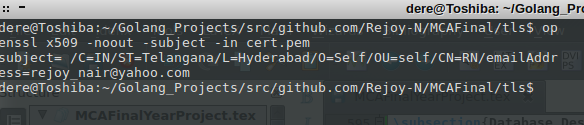
\includegraphics[ width=\textwidth , keepaspectratio ]{./Images/TLScertdetail.png}\\[-1em]
\vspace{0.25cm}
\caption{TLS Certificate Details - 1}
\label{fig:2}
\end{figure}


\begin{sideways}
    \centering
		\begin{minipage}{\textheight}
		\centering
		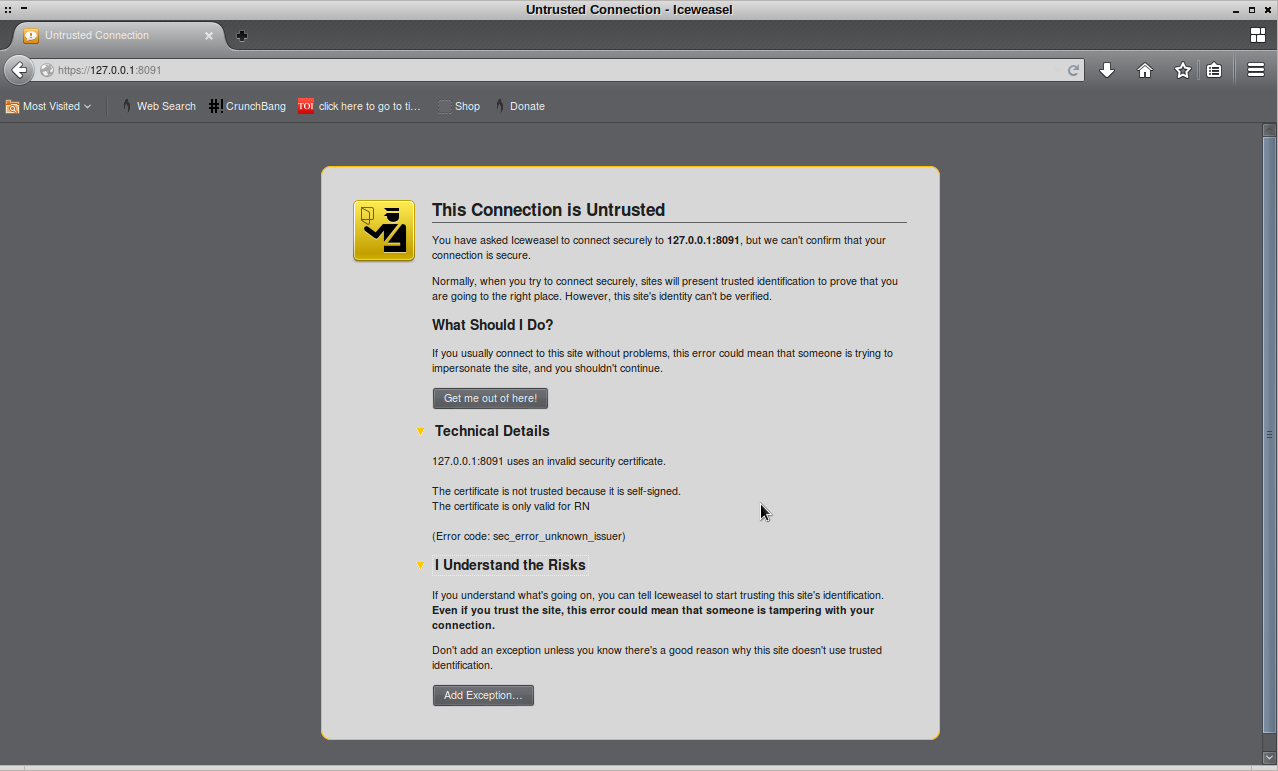
\includegraphics[ width=0.87\textheight , keepaspectratio ]{./Images/TLSSecurityWarning3.png}\\[-1em]
		%\vspace{0.25cm}
		\captionof{figure}{TLS Certificate Details - 2}
		\label{fig:2}
		\end{minipage}
\end{sideways}


\begin{figure}[H]
\centering
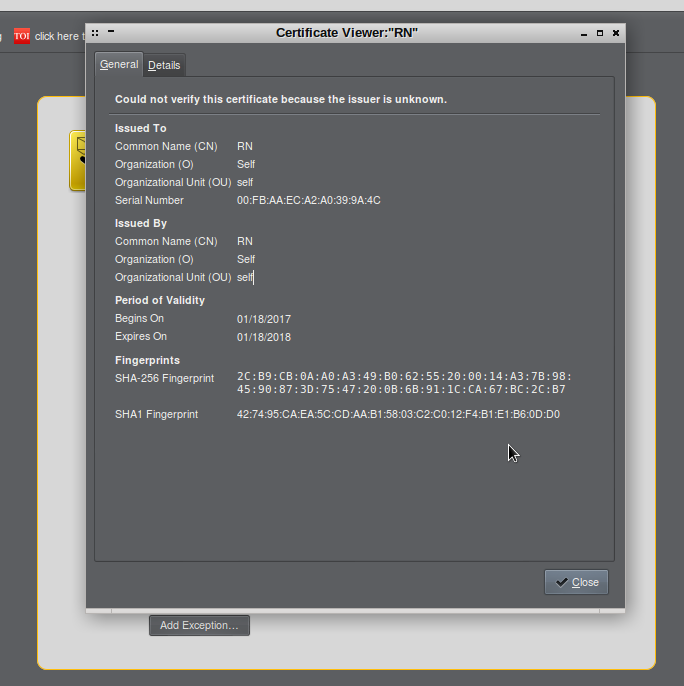
\includegraphics[ width=\textwidth , keepaspectratio ]{./Images/TLSSecurityWarning4.png}\\[-1em]
\vspace{0.25cm}
\caption{TLS Certificate Details - 3}
\label{fig:2}
\end{figure}





The Transport Layer Security protocol aims primarily to provide privacy and data integrity between two communicating computer applications. When secured by TLS, connections between a client (e.g., a web browser) and a server have one or more of the following properties:
\begin{easylist}
& \thinspace The connection is private (or secure) because symmetric cryptography is used to encrypt the data transmitted. The keys for this symmetric encryption are generated uniquely for each connection and are based on a shared secret negotiated at the start of the session. The server and client negotiate the details of which \gls{encryption} \gls{algorithm} and cryptographic keys to use before the first byte of data is transmitted. The negotiation of a shared secret is both secure (the negotiated secret is unavailable to eavesdroppers and cannot be obtained, even by an attacker who places themselves in the middle of the connection) and reliable (no attacker can modify the communications during the negotiation without being detected).
& \thinspace The identity of the communicating parties can be authenticated using public-key cryptography. This authentication can be made optional, but is generally required for at least one of the parties (typically the server).
& \thinspace The connection ensures integrity because each message transmitted includes a message integrity check using a \gls{message authentication code} to prevent undetected loss or alteration of the data during transmission.
\end{easylist}
\bigskip
\noindent

In addition to the properties above, careful configuration of TLS can provide additional privacy-related properties such as \gls{forward secrecy}, ensuring that any future disclosure of encryption keys cannot be used to decrypt any TLS communications recorded in the past.
\\

The TLS protocol comprises two layers: the \gls{TLS record protocol} and the \gls{TLS handshake protocol}.
\\

Since applications can communicate either with or without TLS (or SSL), it is necessary for the client to indicate to the server the setup of a TLS connection. One of the main ways of achieving this is to use a different port number for TLS connections, for example port 443 for \Gls{HTTPS}.
\\

Once the client and server have agreed to use TLS, they negotiate a \gls{stateful connection} by using a handshaking procedure. The protocols use a handshake with an \gls{asymmetric cipher} to establish cipher settings and a shared key for a session; the rest of the communication is encrypted using a \gls{symmetric cipher} and the \gls{session key}. During this \gls{handshake}, the \gls{client} and server agree on various parameters used to establish the connection`s security:

\begin{easylist}
& \thinspace The handshake begins when a client connects to a TLS-enabled server requesting a secure connection and presents a list of supported cipher suites (ciphers and \gls{hash functions}).
& \thinspace From this list, the server picks a cipher and hash function that it also supports and notifies the client of the decision.
& \thinspace The server usually then sends back its identification in the form of a \gls{digital certificate}. The certificate contains the server name, the trusted \Gls{CA} and the server`s public encryption key.
& \thinspace The client confirms the validity of the certificate before proceeding.
& \thinspace To generate the session keys used for the secure connection, the client either:
&& encrypts a random number with the server`s public key and sends the result to the server (which only the server should be able to \gls{decrypt} with its \gls{private key}); both parties then use the random number to generate a unique session key for subsequent encryption and decryption of data during the session
&& uses \Gls{Diffie-Hellman key exchange} to securely generate a random and unique session key for encryption and decryption that has the additional property of \gls{forward secrecy}: if the server`s private key is disclosed in future, it cannot be used to decrypt the current session, even if the session is intercepted and recorded by a third party.
\end{easylist}
\bigskip
\noindent

This concludes the handshake and begins the secured connection, which is encrypted and decrypted with the session key until the connection closes. If any one of the above steps fail, the TLS handshake fails, and the connection is not created.\\

\noindent
\textbf{Digital Certificates} \\
A digital certificate certifies the ownership of a public key by the named subject of the certificate, and indicates certain expected usages of that key. This allows others (relying parties) to rely upon signatures or on assertions made by the private key that corresponds to the certified public key.
\\

TLS typically relies on a set of trusted third-party certificate authorities to establish the authenticity of certificates. Trust is usually anchored in a list of certificates distributed with user agent software and can be modified by the relying party. As a consequence of choosing \Gls{X.509 certificates}, certificate authorities and a public key infrastructure are necessary to verify the relation between a certificate and its owner, as well as to generate, sign, and administer the validity of certificates.
\\


\newpage
%*******************************************SECTION**********************************
\section{\MakeUppercase{Cost Estimation of the Project}}

\noindent
\textbf{Estimate Product Size and Resources} \\
The correlation of program size with development time is only moderately good for engineering teams and organizations. However, for individual engineers, the correlation is generally quite high. Therefore, the PSP starts with engineers estimating the sizes of the products they will personally develop. Then, based on their personal size and productivity data, the engineers estimate the time required to do the work. In
the \Gls{PSP}, these size and resource estimates are made with the \Gls{PROBE} method \textsuperscript{ 7}.
\\

\noindent
\textbf{Size Estimating with PROBE}
PROBE stands for PROxy Based Estimating and it uses proxies or objects as the basis for estimating the likely size of a product. With PROBE, engineers first determine the objects required to build the product described by the conceptual design. Then they determine the likely type and number of methods for each object. They refer to historical data on the sizes of similar objects they have previously developed and use \gls{linear regression} to determine the likely overall size of the finished product. The example object size data in figure below show the five size ranges the PSP uses for objects. Since object size is a function of programming style, the PROBE method shows engineers how to use the data on the programs they have personally developed to generate size ranges for their personal use. Once they have estimated the sizes of the objects, they used linear regression to estimate the total amount of code they plan to develop. To use linear regression, the engineers must have historical data on estimated versus actual program size for at least three prior programs.

\begin{figure}[H]
\centering
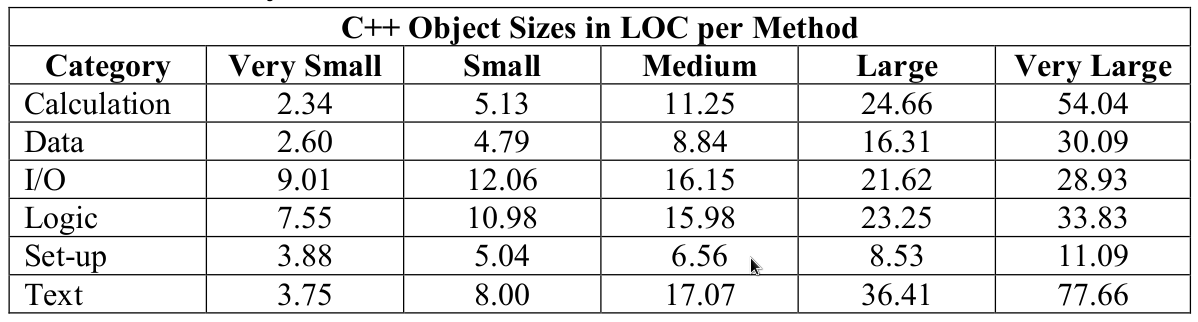
\includegraphics[ width=\textwidth , keepaspectratio ]{./Images/PSPObjectSizeData.png}\\[-1em]
\vspace{0.25cm}
\caption{C\textsuperscript{++} Object Size Data}
\label{fig:2}
\end{figure}

\noindent
Any reference material for Object Size Data for Go Programs was not found. Hence the C\textsuperscript{++} object size data was used in the estimation. \\

\begin{figure}[H]
\centering
\includegraphics[ width=0.7\textwidth , keepaspectratio ]{./Images/Costa.png}\\[-1em]
\vspace{0.25cm}
\caption{Effort details - Go Programs}
\label{fig:2}
\end{figure}

\begin{figure}[H]
\centering
\includegraphics[ width=0.4\textwidth , keepaspectratio ]{./Images/Costb.png}\\[-1em]
\vspace{0.25cm}
\caption{Effort details - HTML/JS Programs}
\label{fig:2}
\end{figure}



\noindent
\textbf{Size Measures : \Gls{LOC}}
Since the time it takes to develop a product is largely determined by the size of that product, when using the PSP, engineers first estimate the sizes of the products they plan to develop. Then, when they are done, they measure the sizes of the products they produced. This provides the engineers with the size data they need to make accurate size estimates. However, for these data to be useful, the size measure must correlate with the development time for the product. While lines of code (LOC) is the principal PSP size measure, any size measure can be used that provides a reasonable \gls{correlation} between development time and product size. It should also permit automated measurement of actual product size.
\\

The PSP uses the term ``logical LOC`` to refer to a logical construct of the programming language being used. Since there are many ways to define logical LOC, engineers must precisely define how they intend to measure LOC. In this project LOC is simply the actual number of lines of codes as provided by the IDE.


\newpage
%*******************************************SECTION**********************************
%\section{\MakeUppercase{Reports}}
%\newpage
%*******************************************SECTION**********************************
\section{\MakeUppercase{Project Chart, Gantt Chart}}

There cannot be a concept of a \Gls{PERT} chart for software development work carried out by a single developer as there is no other option but to carry out the work sequentially. In that sense, the PERT chart and the \Gls{Gantt chart} would be the same. PSP however has methods are introduced in a series of seven process versions. These versions are labeled PSP0 through PSP3, and each version has a similar set of logs, forms, scripts, and standards, as shown in Figure. The process scripts define the steps for each part of the process, the logs and forms provide templates for recording and storing data, and the standards guide the engineers as they do the work.

\begin{figure}[H]
\centering
\includegraphics[ width=\textwidth , keepaspectratio ]{./Images/PSPProcessElements1.png}\\[-1em]
\vspace{0.25cm}
\caption{PSP Process Elements}
\label{fig:2}
\end{figure}


\begin{figure}[H]
\centering
\includegraphics[ width=\textwidth , keepaspectratio ]{./Images/PSPPert1.png}\\[-1em]
\vspace{0.25cm}
\caption{PSP Process Elements in the PSP Process}
\label{fig:2}
\end{figure}

\begin{sideways}
\centering
\begin{minipage}{\textheight}
\begin{center}
			
		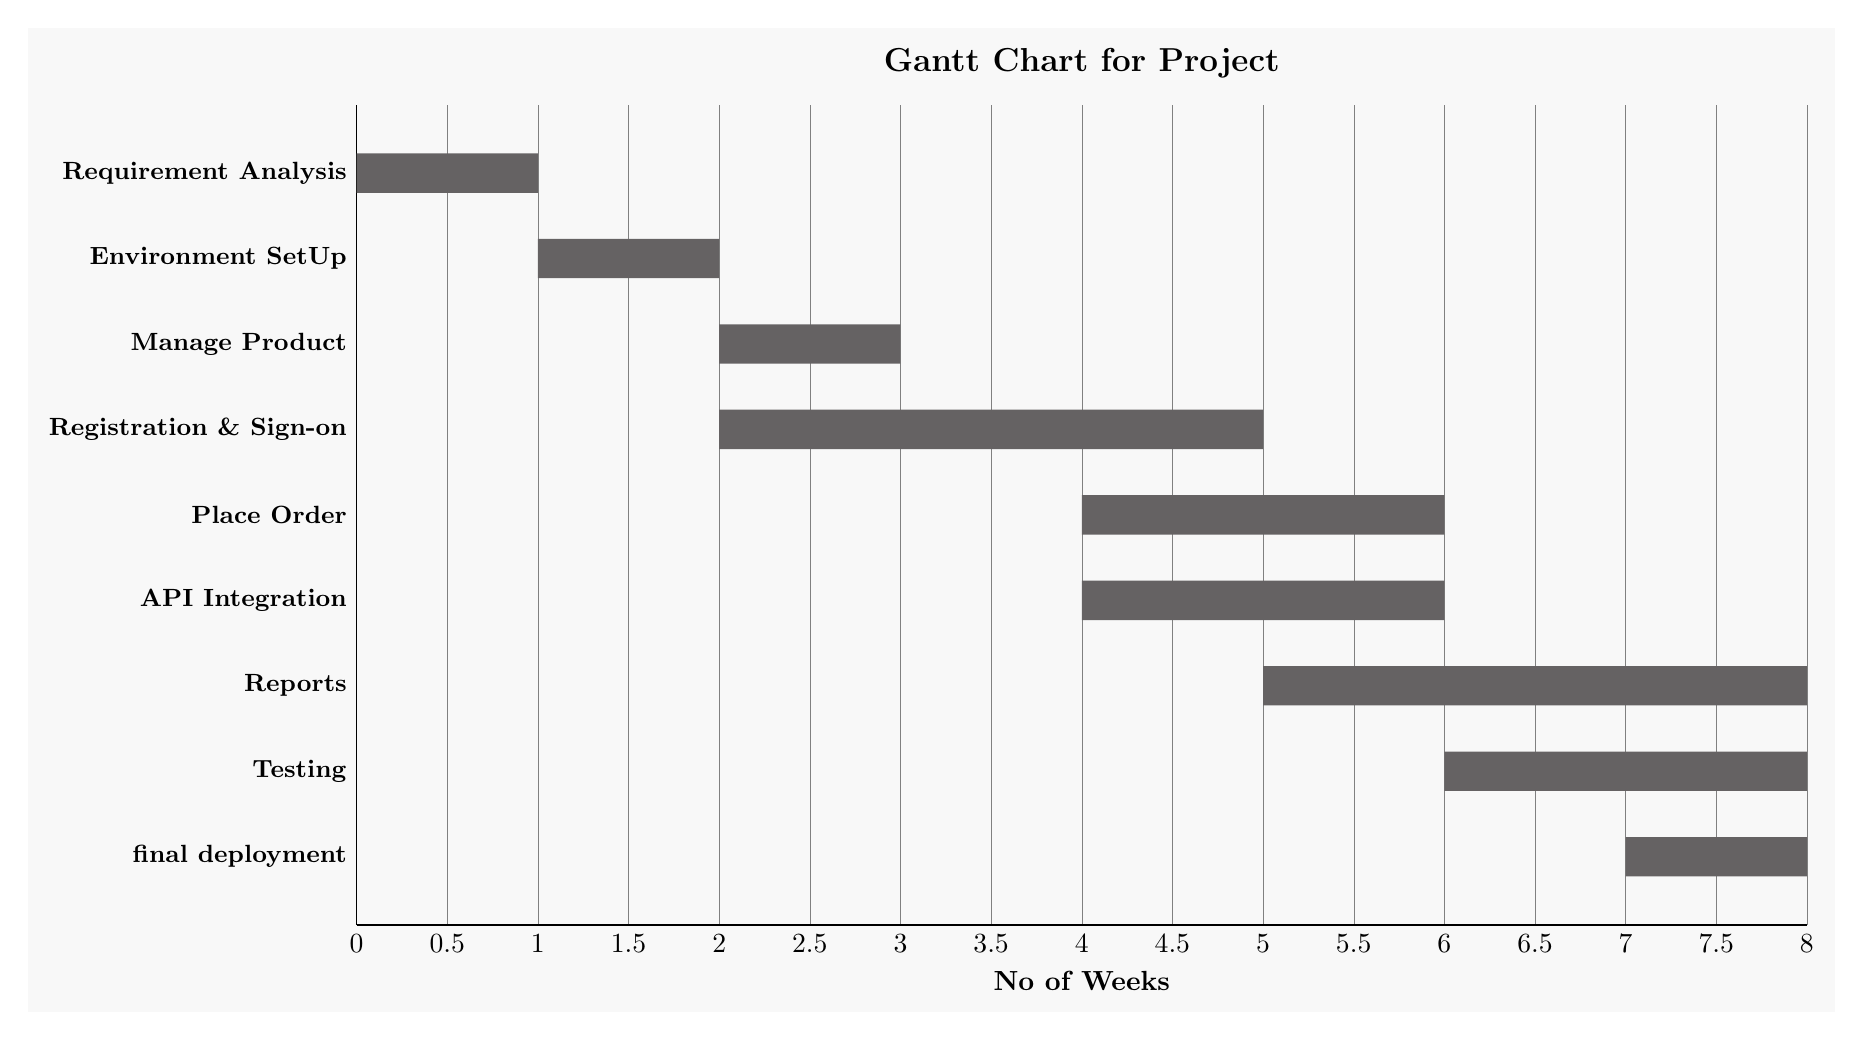
\begin{tikzpicture}[use background]
		
		\pgfplotstableread{ % Read the data into a table macro
			Label                                                      First   Second  
			{\small \textbf{final deployment}}                           7     1
			{\small \textbf{Testing}}                                    6     2
			{\small \textbf{Reports}}                                    5     3
			{\small \textbf{API Integration }}                           4     2
			{\small \textbf{Place Order}}                                4     2
			{\small \textbf{Registration \& Sign-on}}                    2     3
			{\small \textbf{Manage Product}}                             2     1
			{\small \textbf{Environment SetUp}}                          1     1
			{\small \textbf{Requirement Analysis}}                       0     1
		}\datatable
		
		\begin{axis}[
		xbar stacked,   % Stacked horizontal bars
		xmin=0,  xmax=8,       % Start x axis at 0
		title={\large \textbf {Gantt Chart for Project}},
		height=12cm, width=20cm,
		bar width=0.5cm,
		axis x line*=bottom,
		axis y line*=left,
		y axis line style={opacity=1},
		enlarge y limits=true,
		xmajorgrids={true},
		grid style={
			solid,
			ultra thin,
			gray
		},
		tick style={tickwidth=0cm,major tick length=0cm},
		xlabel={\textbf{No of Weeks }},
		ytick=data,     % Use as many tick labels as y coordinates
		yticklabels from table={\datatable}{Label}  % Get the labels from the Label column of the \datatable
		]
		\addplot [draw=none,fill=none] table [x=First, y expr=\coordindex] {\datatable};    % Plot the "First" column against the data index
		\addplot [draw=none,fill={levelfirst}]table [x=Second, y expr=\coordindex] {\datatable};
		
		
		\end{axis}
		
		\end{tikzpicture}
		
\end{center}
\end{minipage}
\end{sideways}

\newpage
%*******************************************SECTION**********************************
\section{\MakeUppercase{Future Scope and further enhancement }}

The existing website can be developed further by adding more functionalities viz.,

\begin{easylist}
& \thinspace Forgot Password functionality that allows users to reset password
& \thinspace Single-Sign On
& \thinspace Use of apt Keywords in Meta-tags that allow fo better results in Google Search
& \thinspace Filter Products
& \thinspace \Gls{persistent} Cart
& \thinspace Cancel Order
& \thinspace Print PDF
& \thinspace Add more Product attributes
& \thinspace Different Modes of Payment Like \Gls{Digital Wallets}
& \thinspace \Gls{Responsive Web Design}
& \thinspace Location services based on Wifi or \Gls{GPS}
& \thinspace Rate \& Review Product
& \thinspace Chat interface
\end{easylist}
\bigskip

\noindent
The above is only an indicative list. Most of the features for retail website can be implemented using Go.\\

\noindent
An important aspect of this project is that the entire development has been done on a i686 m/c equipped with just 512 MB RAM. This is an important factor in increasing functionality and scalability of the web app.

\newpage
%*******************************************SECTION**********************************
\section{\MakeUppercase{Bibliography}}
\noindent
[1] https://en.wikipedia.org/wiki/Online\_shopping \\

\noindent
[2] http://www.indiaretailing.com/2016/08/30/retail/online-shopping-trends-facts-figures-on-indian-e-comm-sector \\

\noindent
[3] https://en.wikipedia.org/wiki/Personal\_software\_process \\

\noindent
[4] https://talks.golang.org/2012/splash.article \\

\noindent
[5] https://en.wikipedia.org/wiki/User\_interface\_design \\

\noindent
[6] https://en.wikipedia.org/wiki/Transport\_Layer\_Security \\

\noindent
[7] Pittsburgh, PA 15213-3890. The Personal. Software. Process. SM. (PSP. SM. ) CMU/SEI-2000-TR-022. ESC-TR-2000-022. Watts S. Humphrey. November 2000.

\newpage

%*******************************************SECTION**********************************
\section{\MakeUppercase{Appendices}}

\renewcommand{\cftfigfont}{Figure }

%\emptypage\listoffigures
\listoffigures
%\listoffigures


\newpage

\renewcommand{\cfttabfont}{Table }

%\emptypage\listoftables
\listoftables

\newpage
%*******************************************SECTION**********************************
\section{\MakeUppercase{Glossary}}

  
\printglossaries

%*******************************************END**********************************


\end{document}